\documentclass[12pt, a4paper, openany]{report}

% ==========================================
% PACKAGES
% ==========================================
\usepackage[utf8]{inputenc}
\usepackage[T1]{fontenc}
\usepackage[french]{babel}
\usepackage[top=3.5cm, bottom=2.5cm, left=2cm, right=2cm, headheight=75pt, headsep=1cm, footskip=1.5cm]{geometry}
\usepackage{graphicx}
\usepackage{tikz}
\usepackage{colortbl}
\usepackage{array}
\usepackage{xcolor}
\usepackage{lmodern}
\usepackage{booktabs}
\usepackage{microtype}
\usepackage{float} % <--- ZID HAD L'PACKAGE HNA
\usepackage{pifont} % <--- ZID HADI HNA
\usepackage{pgfgantt} % Package l-asassi dyal l'Gantt
\usepackage{graphicx} % Bach n-gueddou l'3bar dyalo m3a l'wer9a
\usepackage{pifont}
\usepackage{nicematrix}

\usepackage{titlesec}
\usepackage{etoolbox}
\usepackage{hhline}
\usepackage{enumitem}

% ← ZID HADI: Bach nmanc3o ga3 les pages khawyin
\let\cleardoublepage\clearpage

\makeatletter
\patchcmd{\@chapter}
  {\if@openright\cleardoublepage\else\clearpage\fi}
  {}{}{}
\makeatother

% ==========================================
% DESIGN DES TITRES (Sections, Sous-sections...)
% ==========================================
% Loun dyal Section (Titre kbir b zre9 mghlo9)
\titleformat{\section}
  {\color{primaryBlue}\normalfont\LARGE\bfseries}
  {\thesection}{0.5em}{}

% Loun dyal Subsection (Titre mtwest b zre9 royal)
\titleformat{\subsection}
  {\color{royalBlue}\normalfont\Large\bfseries}
  {\thesubsection}{0.5em}{}

% Loun dyal Subsubsection (Titre sghir b zre9 mftou7)
\titleformat{\subsubsection}
  {\color{azureBlue}\normalfont\large\bfseries}
  {\thesubsubsection}{0.5em}{}

% Espace bin les titres w l'ktba
\titlespacing*{\section}{0pt}{3ex plus 1ex minus .2ex}{2ex plus .2ex}
\titlespacing*{\subsection}{0pt}{2ex plus 1ex minus .2ex}{1.5ex plus .2ex}

% 1. Had l'code bach nkhbiw l'titre dyal \chapter standard BLA maydir page khawya
\titleformat{\chapter}[display]{}{}{0pt}{\vspace*{-3cm}\phantom}
\titlespacing*{\chapter}{0pt}{-30pt}{10pt}

% 2. Had l'code bach l'page li fiha \chapter t7tarem l'footer dyalna (l'khat zre9)
\patchcmd{\chapter}{\thispagestyle{plain}}{\thispagestyle{frontmatter}}{}{}

% ==========================================
% COMMANDE POUR LA PAGE DE GARDE DU CHAPITRE
% ==========================================
\newcommand{\chapterpage}[2]{%
    \clearpage % T-bda page jdida n9iya
    \thispagestyle{frontmatter} 
    \vspace*{\fill}
    \begin{center}
        \begin{tikzpicture}
            % 1. Image kberna liha l'width l 1.15 bach tban kbira w t-ched l'3erd
            \node[inner sep=0pt] (frame) at (0,0) {
                
\includegraphics[width=1.0\textwidth, keepaspectratio]{images/cercle-chapitre.png}
            };
            
            % 2. L'ktba m-centriya
            \node[align=center, text width=0.8\textwidth] at (0,0) {
                {\fontsize{36}{44}\selectfont\color{primaryBlue}\bfseries Chapitre #1}\\[15pt]
                \textcolor{primaryBlue}{\rule{5cm}{2pt}}\\[15pt]
                {\fontsize{24}{32}\selectfont\color{primaryBlue}\bfseries #2}
            };
        \end{tikzpicture}
    \end{center}
    \vspace*{\fill}
    % MSSE7NA \newpage MN HNA BACH MAT3TICH WRATI KHAWYIN
    \newpage % <--- ZID HADI
}

% --- ZID HAD L'PACKAGE HNA BACH YBANO NOQAT F L'FIHRES ---
\usepackage[titles]{tocloft}
\renewcommand{\cftchapleader}{\cftdotfill{\cftdotsep}}
% ---------------------------------------------------------
% Zid had 3 stora bach tktb "Figure X :" f Table des figures:
\renewcommand{\cftfigpresnum}{Figure }
\renewcommand{\cftfigaftersnum}{ :}
\addtolength{\cftfignumwidth}{40pt} % Tissa3 bach t9ed lkelma "Figure 10 :"
% ---------------------------------------------------------

% L'code jdid dyal Liste des tableaux:
\renewcommand{\cfttabpresnum}{Tableau }
\renewcommand{\cfttabaftersnum}{ :}
\addtolength{\cfttabnumwidth}{48pt} % Drnaha 48pt 7it kelmat 'Tableau' twel mn 'Figure'
% ---------------------------------------------------------


% ==========================================
% CUSTOM TABLE DES MATIERES
% ==========================================
\makeatletter
\renewcommand\tableofcontents{%
    \newpage
    \pagestyle{frontmatter}     % <--- ZID HADI: bach tb9a khdama f ga3 l'pages d l'fihres
    \thispagestyle{frontmatter} % <--- BEDDEL HADI: mn 'empty' l 'frontmatter'
    \vspace*{0.5cm}
    
    % 3. Titre "Table des matières"
    \noindent
    \textcolor{royalBlue}{\rule{0.45\textwidth}{1pt}}
    \hfill
    {\fontsize{24}{28}\selectfont\color{royalBlue}\bfseries Table des matières}\par
    \vspace{1.5cm}
    
    % Hna fin LaTeX kay-généri l'fihres bo7do (Lownah b zre9 mftou7)
    {\color{azureBlue} % <--- BEDDELHA L AZURE BLUE
    \@starttoc{toc}%
    }
}
\makeatother

% ==========================================
% CUSTOM TABLE DES FIGURES
% ==========================================
\makeatletter
\renewcommand\listoffigures{%
    \newpage
    \pagestyle{frontmatter}     
    \thispagestyle{frontmatter} 
    \vspace*{0.5cm} 
    
    % 3. Titre "Table des figures"
    \noindent
    \textcolor{royalBlue}{\rule{0.45\textwidth}{1pt}}
    \hfill
    {\fontsize{24}{28}\selectfont\color{royalBlue}\bfseries Table des figures}\par
    \vspace{1.5cm}
    
    % Hna fin LaTeX kay-généri l'fihres d'les figures
    {\color{azureBlue} 
    \@starttoc{lof}% <--- lof katsme3 'List of Figures'
    }
}
\makeatother

% ==========================================
% CUSTOM LISTE DES TABLEAUX
% ==========================================
\makeatletter
\renewcommand\listoftables{%
    \newpage
    \pagestyle{frontmatter}     
    \thispagestyle{frontmatter} 
    \vspace*{0.5cm} 
    
    % 3. Titre "Liste des tableaux"
    \noindent
    \textcolor{royalBlue}{\rule{0.48\textwidth}{1pt}}
    \hfill
    {\fontsize{24}{28}\selectfont\color{royalBlue}\bfseries Liste des tableaux}\par
    \vspace{1.5cm}
    
    % Hna fin LaTeX kay-généri l'fihres d'les tableaux
    {\color{azureBlue} 
    \@starttoc{lot}% <--- lot katsme3 'List of Tables'
    }
}
\makeatother

\usetikzlibrary{calc}

% ==========================================
% COULEURS (Unified Theme)
% ==========================================
\definecolor{primaryBlue}{RGB}{28, 62, 110}    % Single professional dark blue
\definecolor{lightBlue}{RGB}{235, 243, 250}    % Very light blue for table rows
\definecolor{royalBlue}{RGB}{52, 101, 164}
\definecolor{azureBlue}{RGB}{0, 122, 204}      % <--- ZID HADA (Zre9 mftou7 w kayban)

% ==========================================
% LIENS ET CLICKABLE TOC (Fihres Interactif)
% ==========================================
\usepackage{hyperref}
\hypersetup{
    colorlinks=true,
    linkcolor=azureBlue, % <--- BEDDELHA HNA
    urlcolor=azureBlue,  % <--- W HNA
    linktoc=all 
}

% ==========================================
% CUSTOM HEADER / FOOTER (Bulletproof)
% ==========================================
\usepackage{fancyhdr}

% 1. Kan-definiw l'header w l'footer f variables
\newcommand{\mycustomheader}{%
    \noindent
    \begin{minipage}[b]{0.45\textwidth} 
        \raggedright
        
\includegraphics[height=1.0cm]{images/ntt-data-logo.png}
    \end{minipage}
    \hfill
    \begin{minipage}[b]{0.45\textwidth} 
        \raggedleft
        % ZEDNA \raisebox BACH NHEBTO L'LOGO DYAL FST B D-DRA3
        \raisebox{-0.3cm}{
\includegraphics[height=2.2cm]{images/fst-logo.png}}
    \end{minipage}\par
    \vspace{-0.4cm} % <--- ZEDNA L'ESPACE NEGATIF BACH YLSE9 L'KHAT MZYAN
    \noindent
    \begin{tikzpicture}
        \draw[royalBlue, dash pattern=on 5pt off 3pt, line width=0.8pt] (0,0) -- (\textwidth, 0);
    \end{tikzpicture}%
}

\newcommand{\mycustomfooter}{%
    \centering
    \begin{tikzpicture}
        \fill[royalBlue] (-0.45\textwidth, 0) -- (0, 0.05cm) -- (0.45\textwidth, 0) -- (0, -0.05cm) -- cycle;
    \end{tikzpicture}\\[5pt]
    \textcolor{royalBlue}{\textbf{\thepage}}
}

% 2. Kan-appliqiw hadchi 3la ga3 l'pages (Style 'fancy')
\pagestyle{fancy}
\fancyhf{}
\renewcommand{\headrulewidth}{0pt}
\renewcommand{\footrulewidth}{0pt}
\fancyhead[C]{\mycustomheader}
\fancyfoot[C]{\mycustomfooter}

% 3. Kan-appliqiw hadchi 3la l'pages dyal \chapter (Style 'plain')
\fancypagestyle{plain}{%
    \fancyhf{}
    \renewcommand{\headrulewidth}{0pt}
    \renewcommand{\footrulewidth}{0pt}
    \fancyhead[C]{\mycustomheader}
    \fancyfoot[C]{\mycustomfooter}
}

% 4. Kan-appliqiw hadchi 3la l'pages dyal l'fihres (Style 'frontmatter')
\fancypagestyle{frontmatter}{%
    \fancyhf{}
    \renewcommand{\headrulewidth}{0pt}
    \renewcommand{\footrulewidth}{0pt}
    \fancyhead[C]{\mycustomheader}
    \fancyfoot[C]{\mycustomfooter}
}

% ==========================================
% PROFONDEUR DE NUMÉROTATION (Bach tban 2.5.1)
% ==========================================
\setcounter{secnumdepth}{3} % Kat-biyen ra9m f \subsubsection
\setcounter{tocdepth}{3}    % Kat-biyen \subsubsection 7ta f l'Fihres (Table des matières) 

\begin{document}
\pagestyle{empty}

% --- L'pages Romani (I, II, III, IV...) ---
\pagenumbering{Roman}

% ==========================================
% PAGE DE GARDE
% ==========================================
\begin{titlepage}
\vspace*{-2.5cm} % <--- HADI KAT-JER L'PAGE L-FOUQ
\enlargethispage{1.0cm} % <--- HADI KAT-3TI TISSA3 L-TE7T BACH MAYTZADCH PAGE KHAWYA
\centering

% ------------------------------------------
% TOP BLUE BAR
% ------------------------------------------
\begin{tikzpicture}[remember picture]
  % Top accent bar (full width)
  \fill[primaryBlue] (0, 0) rectangle (\textwidth, 0.25cm);
  % Thin lighter line below
  \fill[primaryBlue!60] (0, -0.1cm) rectangle (\textwidth, 0);
\end{tikzpicture}

\vspace{0.3cm}

% Logos + University name row
\begin{minipage}[c]{0.26\textwidth}
    \centering
    
\includegraphics[width=1\linewidth]{images/uae-logo.png}
\end{minipage}
\hfill
\begin{minipage}[c]{0.46\textwidth}
    \centering
    {\fontsize{13}{15}\selectfont\color{primaryBlue}\bfseries UNIVERSITÉ ABDELMALEK ESSAÂDI}\\[4pt]
    {\fontsize{11}{13}\selectfont\color{primaryBlue}\bfseries Faculté des Sciences}\\[6pt]
    \textcolor{primaryBlue}{\rule{5cm}{0.8pt}}\\[4pt]
    {\fontsize{10.5}{12}\selectfont\color{primaryBlue}\textbf{- Tétouan -}}
\end{minipage}
\hfill
\begin{minipage}[c]{0.26\textwidth}
    \centering
    
\includegraphics[width=1\linewidth]{images/fst-logo.png}
\end{minipage}

\vspace{0.4cm}

% Full-width separator
\textcolor{primaryBlue}{\rule{\textwidth}{1pt}}

\vspace{0.4cm}

% ------------------------------------------
% MASTER BADGE  (double rounded frame)
% ------------------------------------------
\begin{tikzpicture}
  % Outer dashed frame
  \node[
    draw=primaryBlue, dashed, rounded corners=14pt,
    inner sep=6pt, line width=1.2pt
  ] (outer) {
    % Inner solid frame
    \begin{tikzpicture}
      \node[
        draw=primaryBlue, rounded corners=10pt,
        inner xsep=24pt, inner ysep=14pt, line width=1pt,
        fill=lightBlue
      ] (inner) {
        \begin{minipage}{0.75\textwidth}
          \centering
          {\fontsize{13}{18}\selectfont\color{royalBlue}\bfseries Master spécialisé}\\[8pt]
          {\fontsize{20}{19}\selectfont\color{primaryBlue}\bfseries INGÉNIERIE INFORMATIQUE (M2I)}
        \end{minipage}
      };
    \end{tikzpicture}
  };
\end{tikzpicture}

\vspace{0.4cm}

% ------------------------------------------
% PFE TITLE
% ------------------------------------------
{\fontsize{15}{18}\selectfont\color{royalBlue}\bfseries MÉMOIRE DU STAGE PROFESSIONNEL\par}

\vspace{0.2cm}

% Decorative dashed rule
\begin{tikzpicture}
  \draw[primaryBlue, dash pattern=on 6pt off 4pt, line width=2pt]
    (0,0) -- (0.75\textwidth, 0);
\end{tikzpicture}

\vspace{0.35cm}

% ------------------------------------------
% PROJECT TITLE
% ------------------------------------------
{\fontsize{20}{25}\selectfont\color{primaryBlue}\bfseries
  Conception et implémentation full-stack
  \\ du module Invoicing pour la plateforme KAFA'AT EMS\par}

\vspace{0.45cm}

% NTT DATA Logo

\includegraphics[width=6.5cm]{images/ntt-data-logo.png}\par

\vspace{0.35cm}

% Decorative dashed rule
\begin{tikzpicture}
  \draw[primaryBlue, dash pattern=on 6pt off 4pt, line width=2pt]
    (0,0) -- (0.75\textwidth, 0);
\end{tikzpicture}

\vspace{0.35cm}

% ------------------------------------------
% AUTHOR BLOCK
% ------------------------------------------
{\fontsize{14}{16}\selectfont\color{royalBlue}\bfseries Présenté par :\par}
\vspace{0.15cm}
{\fontsize{16}{19}\selectfont\color{primaryBlue}\bfseries ED-DAHMANY Redouane\par}

\vspace{0.3cm}

% Decorative dashed rule
\begin{tikzpicture}
  \draw[primaryBlue, dash pattern=on 6pt off 4pt, line width=2pt]
    (0,0) -- (0.75\textwidth, 0);
\end{tikzpicture}

\vspace{0.3cm}

% ------------------------------------------
% DATE
% ------------------------------------------
{\fontsize{14}{16}\selectfont\color{royalBlue}\bfseries
  Date de soutenance :\enspace 01 juillet 2026\par}

\vfill

% ------------------------------------------
% JURY TABLE
% ------------------------------------------
\arrayrulecolor{primaryBlue}
\renewcommand{\arraystretch}{1.6}
\setlength{\arrayrulewidth}{1pt}

\noindent
\begin{tabular}{|l|l|l|l|}
  \hline
  % --- LIGNE D'EN-TÊTE (Header Row) ---
  \rowcolor{primaryBlue}
  \textbf{\color{white}Titre} &
  \textbf{\color{white}Nom et Prénom} &
  \textbf{\color{white}Établissement} &
  \textbf{\color{white}Qualité} \\
  \hline
  % --- DONNÉES DU JURY ---
  \rowcolor{lightBlue}
  \textbf{\color{primaryBlue}Pr.} &
  \textbf{\color{primaryBlue}Amjad Souad} &
  {\color{primaryBlue}\small Faculté des Sciences Tétouan} &
  {\color{primaryBlue}\bfseries Président} \\
  \hline
  \textbf{\color{primaryBlue}Pr.} &
  \textbf{\color{primaryBlue}Naoufal Rtayli} &
  {\color{primaryBlue}\small Faculté des Sciences Tétouan} &
  {\color{primaryBlue}\bfseries Examinateur} \\
  \hline
  \rowcolor{lightBlue}
  \textbf{\color{primaryBlue}Pr.} &
  \textbf{\color{primaryBlue}Benameur Lamiae} &
  {\color{primaryBlue}\small Faculté des Sciences Tétouan} &
  {\color{primaryBlue}\bfseries Encadrant universitaire} \\
  \hline
  \textbf{\color{primaryBlue}Mr.} &
  \textbf{\color{primaryBlue}Saloumi Achraf} &
  {\color{primaryBlue}\small NTT DATA Tétouan} &
  {\color{primaryBlue}\bfseries Encadrant professionnel} \\
  \hline
\end{tabular}

\vspace{0.3cm}

% ------------------------------------------
% BOTTOM BLUE BAR
% ------------------------------------------
\begin{tikzpicture}
  \fill[primaryBlue] (0, 0) rectangle (\textwidth, 0.25cm);
  \fill[primaryBlue!40] (0, 0.25cm) rectangle (\textwidth, 0.35cm);
\end{tikzpicture}

\end{titlepage}

\setcounter{page}{2}

% ==========================================
% PAGE 2 : VERSETS CORANIQUES
% ==========================================
\thispagestyle{empty}

\vspace*{\fill}
\begin{center}
    % FIX: minipage bach tb9a ga3 les images f page wa7da
    \begin{minipage}{\textwidth}
        \centering
        
\includegraphics[width=0.9\textwidth]{images/bismillah.png}\\[1.7cm]
        
\includegraphics[width=0.9\textwidth]{images/rabbi-zidni-ilma.png}\\[1.7cm]
        
\includegraphics[width=0.9\textwidth]{images/sadaqa-allah.png}
    \end{minipage}
\end{center}
\vspace*{\fill}

% ==========================================
% PAGE 3 : DÉDICACE
% ==========================================
\newpage
\thispagestyle{frontmatter} % Bach n7kmo f ra9m l'page b idina lte7t
\phantomsection % <--- ZID HADI HNA
\addcontentsline{toc}{chapter}{Dédicace} % <--- 7ETHA HNA !

\vspace*{0.5cm} % Bach ntle3o l'header lfo9 chwia

% 3. Titre "Dédicace" 3la Limen
\noindent
\textcolor{royalBlue}{\rule{0.65\textwidth}{1pt}}
\hfill
{\fontsize{24}{28}\selectfont\color{royalBlue}\bfseries Dédicace}

\vspace{1.5cm}

% 4. Le Texte (Italique w mkber chwia m3a espace bin stoura)
\begin{large}
\itshape
\setlength{\parskip}{0.3cm} % L'espace bin les paragraphes
\renewcommand{\baselinestretch}{1.3}\selectfont % L'espace bin stoura (interligne)

Je dédie ce travail à mes parents, qui ont été ma source constante d'inspiration, d'amour et de soutien tout au long de ma vie. Leur encouragement inconditionnel et leur confiance en moi ont été les fondements de ma réussite.

Je tiens à exprimer ma profonde reconnaissance envers mes encadrants, le Professeur \textbf{Benameur Lamiae} et Mr. \textbf{Saloumi Achraf}, pour leur accompagnement, leurs conseils précieux et leur expertise tout au long de ce projet. Leur patience, leur disponibilité et leur dévouement ont été des moteurs essentiels de ma progression.

J'adresse également mes remerciements à mes professeurs, qui m'ont transmis leur savoir, m'ont inspiré et ont élargi mes horizons intellectuels. Leurs enseignements ont façonné ma pensée critique et ont contribué à mon développement personnel et académique.

Enfin, je souhaite exprimer ma gratitude envers mes amis, qui ont été mes compagnons de route tout au long de cette aventure. Leur soutien moral, leur encouragement et leur amitié indéfectible m'ont permis de surmonter les obstacles et de persévérer dans mes efforts.

À tous ceux qui ont joué un rôle important dans ma vie académique et professionnelle, je vous adresse mes sincères remerciements et ma profonde reconnaissance. Votre influence et votre soutien continus ont été inestimables et ont contribué à ma réussite.

\end{large}

\vspace{0.6cm}

% 5. Signature
\begin{flushright}
    {\fontsize{14}{16}\selectfont\textit{\textbf{ED-DAHMANY Redouane}}}
\end{flushright}

% \vfill
\vspace{0.1cm}


% ==========================================
% PAGE 4 : REMERCIEMENTS
% ==========================================
\newpage
\thispagestyle{frontmatter} % Bach n7kmo f ra9m l'page b idina lte7t
\phantomsection % <--- ZID HADI HNA
\addcontentsline{toc}{chapter}{Remerciements} % <--- 7ETHA HNA !

\vspace*{0.5cm} % Bach ntle3o l'header lfo9 chwia


% 3. Titre "Remerciements" 3la Limen
\noindent
\textcolor{royalBlue}{\rule{0.55\textwidth}{1pt}}
\hfill
{\fontsize{24}{28}\selectfont\color{royalBlue}\bfseries Remerciements}

\vspace{0.0cm}

% 4. Le Texte (Italique w mkber chwia m3a espace bin stoura)
\begin{large}
\itshape
\setlength{\parskip}{0.3cm} % L'espace bin les paragraphes
\renewcommand{\baselinestretch}{1.3}\selectfont % L'espace bin stoura (interligne)

Je tiens tout d'abord à exprimer ma gratitude à Allah pour m'avoir accordé la santé, la détermination et la persévérance nécessaires pour mener à bien ce travail de recherche.

Ensuite, je tiens à remercier chaleureusement mon encadrante universitaire, le Professeur \textbf{Benameur Lamiae}, pour son soutien constant, ses précieux conseils et son expertise tout au long de ce projet. Sa disponibilité, sa patience et sa bienveillance ont été d'une aide inestimable.

Je souhaite également exprimer ma reconnaissance à Mr. \textbf{Saloumi Achraf}, mon encadrant professionnel au sein de NTT DATA, pour son accompagnement, son expertise et ses conseils avisés. Sa vision et son expérience ont grandement contribué à la réussite de ce projet.

Je tiens à exprimer ma reconnaissance envers l'ensemble de l'équipe de \textbf{NTT DATA Maroc}, et tout particulièrement à Monsieur \textbf{Fred SABBAH}, Directeur Général, pour m'avoir offert l'opportunité de réaliser ce stage dans un environnement professionnel stimulant. Leur confiance en mes capacités et leur soutien ont été essentiels pour l'accomplissement de ce travail.

Je souhaite également remercier les membres du jury, le Professeur \textbf{Amjad Souad} et le Professeur \textbf{Naoufal Rtayli}, d'avoir accepté d'évaluer ce travail.

Enfin, je tiens à exprimer ma gratitude envers ma famille et mes amis pour leur soutien indéfectible, leurs encouragements et leurs précieux conseils tout au long de ce parcours académique.

Mes sincères remerciements à toutes les personnes qui ont contribué de près ou de loin à la réalisation de ce travail.

\end{large}

\vspace{0.6cm}

% \vfill
\vspace{0.1cm}


% ==========================================
% PAGE 5 : RÉSUMÉ
% ==========================================
\newpage
\thispagestyle{frontmatter} % Bach n7kmo f ra9m l'page b idina lte7t
\phantomsection % <--- ZID HADI HNA
\addcontentsline{toc}{chapter}{Résumé} % <--- 7ETHA HNA !

\vspace*{0.5cm} % Bach ntle3o l'header lfo9 chwia

% 3. Titre "Résumé" 3la Limen
\noindent
\textcolor{royalBlue}{\rule{0.65\textwidth}{1pt}}
\hfill
{\fontsize{24}{28}\selectfont\color{royalBlue}\bfseries Résumé}

\vspace{0.0cm}

% 4. Le Texte (Taille normale m3a espace bin stoura)
\begin{large}
\setlength{\parskip}{0.3cm} % L'espace bin les paragraphes
\renewcommand{\baselinestretch}{1.3}\selectfont % L'espace bin stoura (interligne)

Ce rapport présente une synthèse du travail effectué dans le cadre de mon projet de fin d'études au sein de la société \textbf{NTT DATA} à Tétouan, dans le but d'obtenir mon diplôme du Master spécialisé en Ingénierie Informatique (M2I) de la Faculté des Sciences de Tétouan / Université Abdelmalek Essaâdi.

Ce projet s'est déroulé au sein d'une équipe de développement travaillant sur une plateforme d'entreprise à grande échelle. L'objectif principal de ce projet était de concevoir et d'implémenter de bout en bout (Full-Stack) le module complexe de facturation (\textbf{Invoicing}) pour le système de gestion des employés \textbf{KAFA'AT EMS}.

En raison de sa complexité et de sa logique métier pointue, ce module a été traité comme un microservice indépendant. Il prend en charge la gestion financière, les calculs liés aux temps de travail (Worktime overrides), l'application des règles de facturation, et la génération des factures.

L'application a été développée en utilisant le framework \textbf{Angular 17+} pour la partie frontend, garantissant une interface utilisateur réactive et ergonomique. Le backend a été construit avec \textbf{Java} et \textbf{Spring Boot 3.x}, en utilisant \textbf{PostgreSQL} pour la gestion et la persistance des données relationnelles.

La méthodologie adoptée pour la réalisation de ce projet s'est appuyée sur les pratiques agiles, allant de l'étude et la spécification des besoins à la modélisation de l'architecture et des fonctionnalités via le langage UML, pour aboutir à l'intégration et au déploiement du module.

\vspace{0cm}

\noindent\textbf{Mots clés :} \\
Application Web, Plateforme EMS, Invoicing, Microservice, NTT DATA, Angular, Spring Boot, PostgreSQL, Full-Stack.

\end{large}

\vspace{0.0cm}

% \vfill
\vspace{0.1cm}


% ==========================================
% PAGE 6 : ABSTRACT
% ==========================================
\newpage
\thispagestyle{frontmatter} 
\phantomsection % <--- ZID HADI HNA
\addcontentsline{toc}{chapter}{Abstract} % <--- 7ETHA HNA !

\vspace*{0.5cm} 

% 3. Titre "Abstract" 3la Limen
\noindent
\textcolor{royalBlue}{\rule{0.65\textwidth}{1pt}}
\hfill
{\fontsize{24}{28}\selectfont\color{royalBlue}\bfseries Abstract}

\vspace{0.0cm}

% 4. Le Texte (Taille normale m3a espace bin stoura)
\begin{large}
\setlength{\parskip}{0.3cm} % L'espace bin les paragraphes
\renewcommand{\baselinestretch}{1.3}\selectfont % L'espace bin stoura (interligne)

This report presents a summary of the work carried out as part of my graduation project (Master's thesis) at \textbf{NTT DATA} in Tetouan, in order to obtain my specialized Master's degree in Computer Engineering (M2I) from the Faculty of Sciences in Tetouan / Abdelmalek Essaâdi University.

This project took place within a development team working on a large-scale enterprise platform. The main objective of this project was to design and implement from scratch (Full-Stack) the complex \textbf{Invoicing} module for the \textbf{KAFA'AT} Employee Management System (EMS).

Due to its complexity and advanced business logic, this module was treated as an independent microservice. It handles financial management, calculations related to worktime overrides, the application of billing rules, and invoice generation.

The application was developed using the \textbf{Angular 17+} framework for the frontend, ensuring a responsive and ergonomic user interface. The backend was built with \textbf{Java} and \textbf{Spring Boot 3.x}, using \textbf{PostgreSQL} for relational data management and persistence.

The methodology adopted for the realization of this project was based on agile practices, ranging from the study and specification of requirements to the modeling of the architecture and functionalities using UML language, culminating in the integration and deployment of the module.

\vspace{0cm}

\noindent\textbf{Keywords:} \\
Web Application, EMS Platform, Invoicing, Microservice, NTT DATA, Angular, Spring Boot, PostgreSQL, Full-Stack.

\end{large}

\vspace{0.5cm}

\vspace{0.1cm}


% ==========================================
% L'APPEL DYAL TABLE DES MATIERES
% ==========================================
\tableofcontents

% ==========================================
% L'APPEL DYAL TABLE DES FIGURES
% ==========================================
\newpage
\phantomsection
\addcontentsline{toc}{chapter}{Table des figures}
\listoffigures


% ==========================================
% L'APPEL DYAL LISTE DES TABLEAUX
% ==========================================
\newpage
\phantomsection
\addcontentsline{toc}{chapter}{Liste des tableaux}
\listoftables


% ==========================================
% L'APPEL DYAL LISTE DES ABRÉVIATIONS
% ==========================================
\newpage
\thispagestyle{frontmatter}
\phantomsection
\addcontentsline{toc}{chapter}{Liste des abréviations}

\vspace*{0.5cm} 


% 3. Titre "Liste des abréviations" 3la Limen
\noindent
\textcolor{royalBlue}{\rule{0.35\textwidth}{1pt}} % <--- N9ESNA MN T-TOUL DYAL L'KHAT (0.35)
\hfill
\mbox{\fontsize{24}{28}\selectfont\color{royalBlue}\bfseries Liste des abréviations} % <--- MBOX BACH MAYT9SSEMCH

\vspace{1.5cm}

% 4. Le Tableau des abréviations
\begin{center}
\renewcommand{\arraystretch}{1.6} % Tissa3 bin stoura
\setlength{\arrayrulewidth}{1pt}
\arrayrulecolor{primaryBlue}

% Tableau b 2 colonnes (25% l'abréviation, 65% l'signification)
% Tableau b 2 colonnes (25% l'abréviation, 65% l'signification)
\begin{tabular}{|>{\centering\arraybackslash}p{0.25\textwidth}|>{\raggedright\arraybackslash}p{0.65\textwidth}|}
    \hline
    % En-tête dyal l'tableau b zre9 mghlo9 w ktba bida
    \rowcolor{primaryBlue}
    \textbf{\textcolor{white}{Abréviation}} & \textbf{\textcolor{white}{Signification}} \\
    \hline
    
    % --- Les données stfin alphabétiquement ---
    
    \rowcolor{lightBlue}
    % \textbf{ACID} & Atomicity, Consistency, Isolation, Durability (Atomicité, Cohérence, Isolation, Durabilité) \\
    % \hline
    \textbf{API} & Application Programming Interface (Interface de Programmation Applicative) \\
    \hline
    % \rowcolor{lightBlue}
    \textbf{CI/CD} & Continuous Integration / Continuous Deployment (Intégration et Déploiement Continus) \\
    \hline
    % \textbf{CORS} & Cross-Origin Resource Sharing (Partage des Ressources Entre Origines Multiples) \\
    % \hline
    \rowcolor{lightBlue}
    % \textbf{CRUD} & Create, Read, Update, Delete (Créer, Lire, Mettre à jour, Supprimer) \\
    % \hline
    \textbf{DAO} & Data Access Object (Objet d'Accès aux Données) \\
    \hline
    % \rowcolor{lightBlue}
    \textbf{DI} & Dependency Injection (Injection de Dépendances) \\
    \hline
    \rowcolor{lightBlue}
    \textbf{DTO} & Data Transfer Object (Objet de Transfert de Données) \\
    \hline
    % \rowcolor{lightBlue}
    \textbf{EMS} & Employee Management System (Système de Gestion des Employés) \\
    \hline
    % \textbf{FST} & Faculté des Sciences de Tétouan \\
    % \hline
    \rowcolor{lightBlue}
    \textbf{HTTP} & HyperText Transfer Protocol (Protocole de Transfert Hypertexte) \\
    \hline
    \textbf{IDE} & Integrated Development Environment (Environnement de Développement Intégré) \\
    \hline
    \rowcolor{lightBlue}
    \textbf{IoC} & Inversion of Control (Inversion de Contrôle) \\
    \hline
    \textbf{JPA} & Java Persistence API \\
    \hline
    \rowcolor{lightBlue}
    \textbf{JSON} & JavaScript Object Notation \\
    \hline
    \textbf{JWT} & JSON Web Token (Jeton Web JSON) \\
    \hline
    \rowcolor{lightBlue}
    \textbf{MVC} & Model-View-Controller (Modèle-Vue-Contrôleur) \\
    \hline
    \textbf{ORM} & Object-Relational Mapping (Mappage Objet-Relationnel) \\
    \hline
    \rowcolor{lightBlue}
    % \textbf{PFE} & Projet de Fin d'Études \\
    % \hline
    \textbf{REST} & Representational State Transfer \\
    \hline
    % \rowcolor{lightBlue}
    \textbf{SGBDR} & Système de Gestion de Base de Données Relationnelle (ex: PostgreSQL) \\
    \hline
    \rowcolor{lightBlue}
    \textbf{SPA} & Single Page Application (Application Web Monopage) \\
    \hline
    % \rowcolor{lightBlue}
    \textbf{SQL} & Structured Query Language (Langage de Requête Structurée) \\
    \hline
    % \textbf{UI/UX} & User Interface / User Experience (Interface Utilisateur / Expérience Utilisateur) \\
    % \hline
    \rowcolor{lightBlue}
    \textbf{UML} & Unified Modeling Language (Langage de Modélisation Unifié) \\
    \hline
\end{tabular}
\end{center}



% ==========================================
% DÉBUT DU CONTENU PRINCIPAL (Page 1, 2, 3...)
% ==========================================
\newpage
\pagenumbering{arabic} % Ar9am 1, 2, 3...
\pagestyle{frontmatter} % N-appliquant l'footer dyalna m3a l'khat zre9


% ==========================================
% INTRODUCTION GÉNÉRALE
% ==========================================
\phantomsection
\addcontentsline{toc}{chapter}{Introduction générale}

\vspace*{0.5cm} 


% 3. Titre "Introduction générale" 3la Limen
\noindent
\textcolor{royalBlue}{\rule{0.3\textwidth}{1pt}}
\hfill
\mbox{\fontsize{24}{28}\selectfont\color{royalBlue}\bfseries Introduction générale}

\vspace{1.0cm}

% 4. Le Texte de l'introduction (Taille normale bach t9ed f 1 page)
\setlength{\parskip}{0.2cm}
\renewcommand{\baselinestretch}{1.2}\selectfont

La transformation digitale et l'optimisation continue des processus de gestion interne sont devenues des enjeux majeurs pour les entreprises cherchant à maintenir leur compétitivité. Dans cette optique, \textbf{NTT DATA}, leader mondial des services informatiques, s'engage à innover et à moderniser ses propres systèmes d'information. C'est dans ce contexte que s'inscrit notre projet de fin d'études, intitulé : 

\begin{center}
    \textcolor{primaryBlue}{\textbf{\og Conception et implémentation full-stack du module Invoicing pour la plateforme KAFA'AT EMS \fg{}.}}
\end{center}

Ce projet, réalisé au sein de \textbf{NTT DATA Tétouan}, a pour but de concevoir et développer de bout en bout un nouveau microservice indépendant dédié à la facturation (\textbf{Invoicing}). Ce module a pour objectif d'automatiser la gestion financière, de traiter les calculs liés aux temps de travail, d'appliquer les règles de facturation, et de générer les factures de manière automatisée, fiable et performante.

Afin de détailler les différentes phases de réalisation de ce projet, le présent rapport est articulé autour de trois chapitres principaux :

\vspace{0.5cm}

% 5. DESIGN ATTRACTIF L'CHAPITRES (Badges TikZ + Tableau invisible)
\noindent
\renewcommand{\arraystretch}{2.0}
\begin{tabular}{@{} m{0.20\textwidth} m{0.72\textwidth} @{}}
    
    \tikz{\node[fill=primaryBlue, text=white, rounded corners=6pt, inner sep=8pt, text width=2.5cm, align=center] {\textbf{Chapitre 1}};} & 
    Introduit l'organisme d'accueil (\textbf{NTT DATA}), le contexte général du projet pour la plateforme \textbf{KAFA'AT EMS}, et détaille la méthodologie de travail adoptée (Agile Scrum).\\
    
    \tikz{\node[fill=royalBlue, text=white, rounded corners=6pt, inner sep=8pt, text width=2.5cm, align=center] {\textbf{Chapitre 2}};} & 
    Consacré à la spécification des besoins, à l'étude fonctionnelle et à la \textbf{conception} technique. Il détaille les choix d'architecture orientée \textbf{Microservices} et la modélisation \textbf{UML} du système.\\
    
    \tikz{\node[fill=azureBlue, text=white, rounded corners=6pt, inner sep=8pt, text width=2.5cm, align=center] {\textbf{Chapitre 3}};} & 
    Se concentre sur la \textbf{réalisation}. Il détaille l'environnement technologique (\textbf{Angular, Spring Boot, PostgreSQL}) et présente les interfaces réalisées.\\
    
\end{tabular}

\vspace{0.6cm}
Ce rapport offre ainsi une vue d'ensemble complète du cycle de vie du développement de ce module, en mettant en évidence les défis techniques relevés et la valeur ajoutée apportée au système global de l'entreprise.


% --- CHAPITRE 1 : START ---
\chapterpage{1}{Contexte général du projet} % Page dyal l'image Gemini
\chapter{Contexte général du projet} % Darouri bach ytzad f l'Fihres

\vspace*{0.8cm} % <--- ZID HADI HNA BACH TB3ED "INTRODUCTION" 3LA L'KHAT ZRE9

% ==========================================
% INTRODUCTION DU CHAPITRE
% ==========================================
% \section* kat3ni section bla ra9m (bla mayktb 1. Introduction)
\section*{Introduction}
\addcontentsline{toc}{section}{Introduction}

\vspace{-0.4cm}
Dans ce premier chapitre, nous allons situer notre projet de fin d'études dans son contexte général. Nous commencerons par présenter l'organisme d'accueil, \textbf{NTT DATA}, au sein duquel ce travail a été réalisé. Ensuite, nous définirons le cadre du projet en détaillant la problématique, la solution proposée pour le module \textbf{Invoicing}, et les objectifs visés. Enfin, nous aborderons la méthodologie de travail mise en place pour assurer le bon déroulement et la planification du projet.

% ==========================================
% SECTION 1 : ORGANISME D'ACCUEIL
% ==========================================
\vspace{-0.4cm}
\section{Présentation de l'organisme d'accueil}
\vspace{-0.5cm}
\subsection{Présentation générale de NTT DATA}

\vspace{-0.3cm}
\textbf{NTT DATA} est une entreprise multinationale de services informatiques et de conseil, faisant partie du groupe NTT (\textit{Nippon Telegraph and Telephone Corporation}), l'un des plus grands conglomérats de télécommunications au monde. Fondée au Japon en 1967, NTT DATA fournit une gamme complète de services informatiques et de solutions technologiques à ses clients à travers le monde.

En tant que fournisseur global, l'entreprise propose une large gamme de services pour aider ses clients à transformer leurs activités. Ces services comprennent le conseil en stratégie, l'intégration de systèmes, le développement et la maintenance d'applications, la gestion de l'infrastructure, ainsi que des services liés au \textit{cloud computing} et à l'analyse de données.

NTT DATA se positionne comme un partenaire stratégique pour ses clients, en leur fournissant des solutions technologiques innovantes basées sur des technologies émergentes. L'entreprise s'appuie sur son expertise technique et son expérience mondiale pour aider ses clients à améliorer leur efficacité opérationnelle, innover et rester compétitifs sur le marché.

\vspace{0.0cm}
% --- INSERTION DU LOGO ---
\begin{figure}[htbp]
    \vspace{0.5cm}
    \centering
    
\includegraphics[width=0.6\textwidth]{images/ntt-data-logo-global.png}
    \vspace{-0.4cm}
    \caption{Logo officiel de l'organisme d'accueil NTT DATA}
    \label{fig:ntt_logo}
    \vspace{0.5cm}
\end{figure}

\vspace{-0.9cm}
\subsection{Historique NTT DATA}

\vspace{-0.3cm}
Avant de plonger dans l'historique détaillé de NTT DATA, il convient de noter que l'entreprise a connu une croissance et une évolution significatives depuis sa création en 1967. De ses modestes débuts en tant que filiale de NTT, NTT DATA est devenue une entreprise mondiale de premier plan dans le secteur des services informatiques et du conseil. Voici une figure des étapes clés de son parcours historique :

\vspace{0.2cm}
% --- INSERTION DE L'IMAGE HISTORIQUE ---
\begin{figure}[htbp]
    \centering
    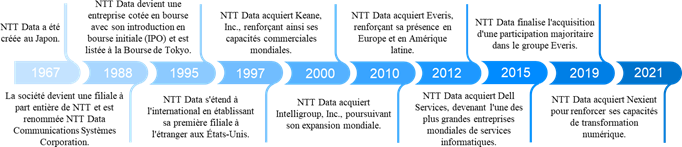
\includegraphics[width=1.0\textwidth]{images/historique-ntt-data.png}
    \vspace{-0.9cm}
    \caption{Historique NTT DATA}
    \label{fig:historique_ntt}
\end{figure}

\vspace{-0.4cm}
Aujourd'hui, NTT DATA est reconnue comme l'un des leaders mondiaux des services informatiques et du conseil, offrant des solutions technologiques innovantes à ses clients dans le monde entier.

\vspace{-0.4cm}
\subsection{Fiche technique}
\vspace{-0.3cm}
Le tableau ci-dessous résume les informations générales et juridiques de l'entreprise :

\vspace{-0.2cm}
% --- TABLEAU FICHE TECHNIQUE (Fusion Global & Maroc) ---
\begin{table}[H]
    \centering
    \renewcommand{\arraystretch}{1.6} % Tissa3 bin stoura
    \setlength{\arrayrulewidth}{1pt}
    \arrayrulecolor{primaryBlue}
    
    \begin{tabular}{|>{\centering\arraybackslash}p{0.28\textwidth}|>{\raggedright\arraybackslash}p{0.62\textwidth}|}
        \hline
        \rowcolor{primaryBlue}
        \textbf{\textcolor{white}{Caractéristique}} & \textbf{\textcolor{white}{Information}} \\
        \hline
        
        \rowcolor{lightBlue}
        \textbf{Raison Sociale / Nom} & NTT DATA \\
        \hline
        
        \textbf{Forme Juridique} & 
        \textbf{Global :} Société commerciale / Société civile \newline 
        \textbf{Maroc :} Société à Responsabilité Limitée (SARL) \\
        \hline
        
        \rowcolor{lightBlue}
        \textbf{Date de Création} & 1\textsuperscript{er} juillet 1988 \\
        \hline
        
        \textbf{Directeur Général} & 
        \textbf{Global :} Yo Honma \newline 
        \textbf{Maroc :} Fred Sabbah \\
        \hline
        
        \rowcolor{lightBlue}
        \textbf{Siège Social \& Adresse} & 
        \textbf{Global :} Tokyo, Japan \newline 
        \textbf{Maroc :} Parc de Tetouanshore, Route de Cabo Negro - Martil \\
        \hline
        
        \textbf{Taille de l'entreprise} & Grande \\
        \hline
        
        \rowcolor{lightBlue}
        \textbf{Activités} & Services informatiques mondiaux, développement de logiciels, gestion des systèmes d'information, externalisation des processus métier. L'étude, la réalisation et la mise en œuvre de solutions d'automatisation pour le secteur privé et les administrations publiques. \\
        \hline
    \end{tabular}
    \vspace{0.0cm}
    \caption{Fiche technique globale et locale de NTT DATA}
    \label{tab:fiche_technique}
\end{table}

\subsection{Couverture mondiale NTT DATA}

\vspace{-0.3cm}
NTT DATA possède une vaste couverture mondiale avec des bureaux et des centres de prestation de services dans de nombreux pays à travers le monde.

% --- IMAGE COUVERTURE MONDIALE ---
\begin{figure}[H] % <--- [H] bach tb9a l'image nichan hna
    \centering
    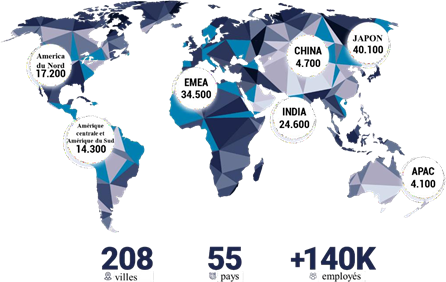
\includegraphics[width=0.80\textwidth]{images/couverture-mondiale.png}
    \vspace{-0.4cm}
    \caption{Couverture mondiale NTT DATA}
    \label{fig:couverture_mondiale}
\end{figure}

\vspace{-0.8cm}
\subsection{Secteur d'activités}

\vspace{-0.3cm}
NTT DATA opère dans le secteur des services informatiques et du conseil. L'entreprise propose une gamme complète de services et de solutions technologiques pour aider ses clients à résoudre leurs défis informatiques et à atteindre leurs objectifs commerciaux. Voici quelques-uns des principaux secteurs d'activité dans lesquels NTT DATA est impliquée :

% --- L'CODE DYAL LES POINTS (DESIGN PRO W JDIID) ---
\begin{itemize}
    % 1. Tissa3 bin n9ati bach mayjich z7am
    \setlength{\itemsep}{0.3cm} 
    
    % 2. Design dyal n9ati (Morba3 sghir zre9 f blast no9ta 3adiya)
    \renewcommand{\labelitemi}{\textcolor{royalBlue}{\rule{1.2ex}{1.2ex}}} 
    
    \vspace{-0.3cm}
    % 3. Lwenna l'Bold b zre9 mghlo9 bach yban w y3ti l'3in
    \item \textcolor{primaryBlue}{\textbf{Services financiers :}} NTT DATA travaille avec des institutions financières, des banques, des compagnies d'assurance et d'autres acteurs du secteur financier pour fournir des solutions informatiques et des services de conseil qui améliorent l'efficacité opérationnelle, la gestion des risques, l'expérience client et la conformité réglementaire.
    
    \vspace{-0.3cm}
    \item \textcolor{primaryBlue}{\textbf{Santé et sciences de la vie :}} NTT DATA fournit des solutions technologiques aux fournisseurs de soins de santé, aux compagnies pharmaceutiques et aux organismes de recherche médicale. Cela inclut la gestion des dossiers médicaux électroniques, les systèmes de gestion des soins de santé, l'analyse des données de santé, les services de télémédecine et les solutions de suivi des essais cliniques.

    \vspace{-0.3cm}
    \item \textcolor{primaryBlue}{\textbf{Secteur public :}} NTT DATA travaille en étroite collaboration avec les gouvernements et les organismes du secteur public pour fournir des solutions informatiques et des services de conseil qui améliorent la prestation des services publics, la gestion des données, la sécurité publique, la gestion des ressources et l'efficacité administrative.

    \vspace{-0.3cm}
    \item \textcolor{primaryBlue}{\textbf{Secteur manufacturier et automobile :}} NTT DATA offre des solutions technologiques aux fabricants et aux entreprises automobiles pour optimiser les opérations de fabrication, améliorer la chaîne d'approvisionnement, intégrer l'Internet des objets (IoT) dans les processus de production et développer des solutions de mobilité intelligente.

    \vspace{-0.3cm}
    \item \textcolor{primaryBlue}{\textbf{Télécommunications et médias :}} NTT DATA collabore avec les fournisseurs de services de télécommunications et les entreprises médiatiques pour fournir des solutions d'infrastructure informatique, des services de transformation numérique, des solutions d'analyse des données, des plateformes de services en ligne et des solutions de gestion des clients.
\end{itemize}

\vspace{-0.3cm}

Outre ces secteurs spécifiques, NTT DATA travaille également avec des entreprises de diverses industries, telles que l'énergie, les transports, le commerce de détail, l'industrie du voyage et de l'hôtellerie, pour fournir des services informatiques et des solutions personnalisées adaptées à leurs besoins spécifiques. [3]

\vspace{0.0cm}

% --- IMAGE DES SECTEURS D'ACTIVITÉS ---
\begin{figure}[H] % <--- [H] bach tb9a l'image nichan hna ta7t l'ktaba
    \centering
    
\includegraphics[width=0.85\textwidth]{images/secteurs-activites.png}
    \vspace{-0.4cm}
    \caption{Quelques secteurs d'activités de NTT DATA}
    \label{fig:secteurs_activites}
\end{figure}

\vspace{-0.9cm}
\subsection{Services offerts par NTT DATA}

\vspace{-0.3cm}
NTT DATA, en tant que fournisseur mondial de services informatiques de confiance, propose une gamme complète de services pour aider les entreprises à relever les défis numériques et à innover. La figure suivante montre les services offerts par société NTT DATA [4]

\vspace{0.1cm}

% --- IMAGE DES SERVICES NTT DATA ---
\begin{figure}[H]
    \centering
    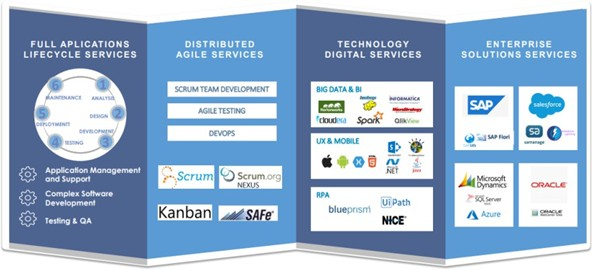
\includegraphics[width=0.85\textwidth]{images/services-ntt-data.png}
    \vspace{-0.4cm}
    \caption{NTT DATA Services}
    \label{fig:services_ntt_data}
\end{figure}

\vspace{0.3cm}

\subsection{Partenaires stratégiques de NTT DATA}

\vspace{-0.3cm}
NTT DATA a établi des partenariats stratégiques avec de nombreuses entreprises leaders dans le domaine de la technologie et des services. Ces partenariats sont essentiels pour renforcer l'offre de solutions de NTT DATA et offrir une valeur ajoutée à ses clients. Parmi les partenaires clés figurent des géants de l'industrie tels que Microsoft, Oracle, SAP, Salesforce, IBM et Amazon Web Services (AWS). Ces partenariats permettent à NTT DATA d'accéder aux dernières technologies et d'offrir des solutions innovantes dans des domaines tels que le cloud computing, les logiciels d'entreprise, la gestion de la relation client, l'analyse des données et bien plus encore. Grâce à ces partenariats stratégiques, NTT DATA peut offrir des services de conseil, d'intégration et de gestion des solutions basées sur les plateformes et les technologies de ses partenaires, répondant ainsi aux besoins variés de ses clients dans divers secteurs d'activité. [5]

\vspace{0.1cm}
% --- IMAGE DES PARTENAIRES STRATÉGIQUES ---
\begin{figure}[H]
    \centering
    
\includegraphics[width=0.85\textwidth]{images/partenaires-ntt-data.png}
    \vspace{-0.4cm}
    \caption{Partenaires stratégiques de NTT DATA}
    \label{fig:partenaires_ntt_data}
\end{figure}

\vspace{-0.8cm}

\subsection{Clients de NTT DATA}

\vspace{-0.3cm}
Les clients de NTT DATA comprennent une vaste gamme d'entreprises et d'organisations à travers le monde. Grâce à son expertise technologique et à ses solutions innovantes, NTT DATA a su établir des partenariats durables avec des clients dans divers secteurs tels que la finance, les télécommunications, la santé, la fabrication et bien d'autres. Que ce soit pour des grandes entreprises internationales ou des entreprises locales, NTT DATA s'engage à fournir des services de haute qualité, adaptés aux besoins spécifiques de chaque client. L'objectif principal est de créer des relations de confiance à long terme et de contribuer à la réussite et à la croissance de ses clients. Voici quelques-uns des clients principaux de NTT DATA : [3]

\vspace{0.1cm}

% --- IMAGE DES CLIENTS ---
\begin{figure}[H]
    \centering
    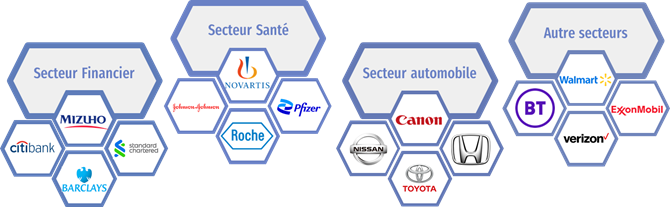
\includegraphics[width=0.9\textwidth]{images/clients-ntt-data.png}
    \vspace{-0.4cm}
    \caption{client NTT DATA}
    \label{fig:clients_ntt_data}
\end{figure}

\subsection{Technologie utilisée par NTT DATA}

\vspace{-0.3cm}
NTT DATA utilise un large éventail de technologies pour exécuter et faire évoluer les services d'application pour ses clients. Parmi les technologies clés utilisées figurent Java, .NET, SQL, Cobol, le testing (tests logiciels) ainsi que la RPA (Robotic Process Automation). Ces technologies sont mises en œuvre par une équipe hautement qualifiée et talentueuse, spécialisée non seulement dans les aspects techniques, mais aussi dans les connaissances sectorielles. En combinant ces technologies de pointe avec une expertise sectorielle approfondie, NTT DATA est en mesure de fournir des solutions innovantes et adaptées aux besoins spécifiques de ses clients, tout en garantissant une qualité élevée et une productivité optimale dans la réalisation de leurs projets d'application. [6]

\vspace{0.4cm}

% --- IMAGE DES TECHNOLOGIES ---
\begin{figure}[H]
    \centering
    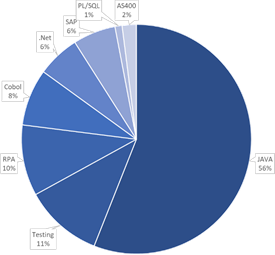
\includegraphics[width=0.85\textwidth]{images/technologies-ntt-data.png}
    \vspace{-0.4cm}
    \caption{Technologie utilisée par NTT DATA}
    \label{fig:technologies_ntt_data}
\end{figure}

\vspace{0.4cm}

\subsection{NTT DATA Maroc}

\vspace{-0.3cm}
NTT DATA est également présent au Maroc. NTT DATA Maroc est une filiale de NTT DATA Corporation, fournisseur mondial de services informatiques et de solutions technologiques. L'entreprise offre une gamme complète de services, notamment le développement de logiciels, la gestion des infrastructures informatiques, les services de conseil en technologie, la transformation numérique et bien plus encore.

NTT DATA Maroc travaille avec des clients locaux et internationaux dans divers secteurs d'activité tels que la finance, les télécommunications, la santé, l'industrie manufacturière, le secteur public, le commerce de détail et d'autres industries. L'objectif de NTT DATA Maroc est d'aider les entreprises à optimiser leurs opérations, à améliorer leur efficacité et à relever les défis technologiques auxquels elles sont confrontées.

En tant que filiale de NTT DATA Corporation, NTT DATA Maroc bénéficie de l'expertise et de l'expérience mondiale de l'entreprise dans le domaine des technologies de l'information. Cela lui permet de proposer des solutions de pointe et d'innover dans le domaine des services informatiques pour répondre aux besoins spécifiques du marché marocain.

NTT DATA Maroc contribue également à l'écosystème technologique du pays en collaborant avec des partenaires locaux, des universités et des institutions pour promouvoir l'innovation, le développement des compétences et la croissance du secteur des technologies de l'information au Maroc. [7]

\vspace{-0.3cm}

\subsection{Organigramme de NTT DATA Maroc}

\vspace{-0.3cm}
L'organigramme de NTT DATA Maroc offre une représentation visuelle de la structure interne de l'entreprise, mettant en évidence les départements, les responsabilités et les relations hiérarchiques qui existent au sein de l'organisation.

\vspace{-0.2cm}

% --- IMAGE DE L'ORGANIGRAMME ---
\begin{figure}[H]
    \centering
    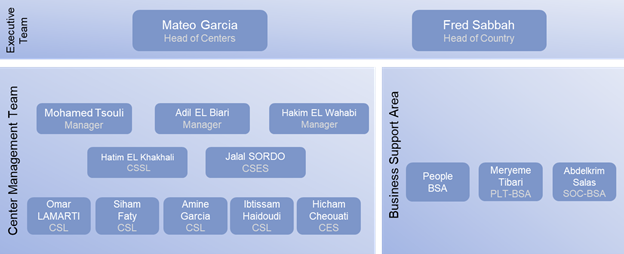
\includegraphics[width=1.0\textwidth]{images/organigramme-ntt-data.png}
    \vspace{-0.9cm}
    \caption{Organigramme de NTT DATA Maroc}
    \label{fig:organigramme_ntt_data_maroc}
\end{figure}

\vspace{-0.4cm}

\subsection{Modèle de carrière}

\vspace{-0.3cm}
NTT DATA utilise un modèle de carrière pour permettre aux employés de développer leurs compétences, de progresser professionnellement et d'atteindre leurs objectifs professionnels au sein de l'entreprise.

Le modèle de carrière de NTT DATA se caractérise par les aspects suivants :

\vspace{0.1cm}

% --- IMAGE MODÈLE DE CARRIÈRE ---
\begin{figure}[H]
    \centering
    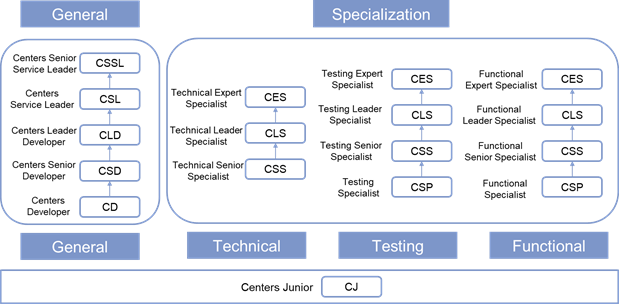
\includegraphics[width=1.0\textwidth]{images/modele-carriere.png}
    \vspace{-0.8cm}
    \caption{Modèle de carrière}
    \label{fig:modele_carriere}
\end{figure}

\vspace{-0.9cm}

% ==========================================
% SECTION 2 : CADRE GÉNÉRAL DU PROJET
% ==========================================
\section{Cadre général du projet}

\vspace{-0.5cm}
\subsection{Contexte du projet}

\vspace{-0.3cm}
Ce projet s'inscrit dans le cadre de la modernisation et de l'optimisation continue des systèmes d'information internes de l'entreprise. NTT DATA dispose d'une plateforme globale et centralisée pour la gestion de ses collaborateurs nommée \textbf{KAFA'AT EMS} (Employee Management System). 

Afin d'étendre les capacités de cette plateforme et de répondre aux exigences croissantes en matière de gestion financière, l'entreprise souhaite concevoir et développer de zéro un nouveau module complet et indépendant dédié à la facturation : le module \textbf{Invoicing}. Ce projet, réalisé au sein des équipes de développement de NTT DATA Tétouan, vise à doter la plateforme EMS d'un outil puissant pour automatiser et fiabiliser le cycle de facturation basé sur les temps de travail et les prestations des employés.

\vspace{0.2cm}

\subsection{Problématique}

\vspace{-0.4cm}
La gestion de la facturation dans une multinationale de l'envergure de NTT DATA est un processus complexe. Elle implique le traitement d'une quantité massive de données croisées : les profils des employés, les assignations aux projets, les taux journaliers, et surtout les temps de travail réels ainsi que leurs ajustements (Worktime overrides).

Actuellement, l'absence d'un module centralisé et automatisé intégré directement à la plateforme EMS peut entraîner plusieurs défis. Les processus manuels ou l'utilisation d'outils fragmentés augmentent considérablement le risque d'erreurs de calcul, créent des goulots d'étranglement administratifs et provoquent des retards dans l'émission des factures. De plus, l'application manuelle de règles de facturation spécifiques à chaque client ou projet est fastidieuse et rend difficile le suivi financier en temps réel.

La problématique majeure réside donc dans la conception d'une solution technique robuste capable de surmonter ces défis. Comment concevoir et implémenter un microservice Full-Stack évolutif qui s'intègre harmonieusement avec l'écosystème KAFA'AT EMS existant, tout en garantissant un calcul exact des données financières et en offrant aux gestionnaires une interface fluide, réactive et sécurisée pour la génération des factures ?

Cependant, dans le cadre de la gestion financière actuelle, les équipes chargées de la facturation rencontrent souvent des difficultés liées à la manipulation de fichiers Excel complexes et à la fragmentation des données. En particulier, lorsque le nombre de collaborateurs et de projets est important, il devient extrêmement difficile de consolider les heures travaillées (Worktime) et d'appliquer les ajustements de manière précise et rapide sans risquer l'erreur humaine.

De plus, le volume des données à traiter à la fin de chaque cycle de facturation nécessite une attention particulière et un temps considérable. À ce stade, il est primordial de trouver une solution technique qui facilite le travail des gestionnaires de manière efficace et moderne, en simplifiant les calculs complexes. Cette solution devrait permettre de générer des factures précises et conformes aux règles métier en quelques clics seulement.

\vspace{-0.4cm}

\subsection{Solution proposée}

\vspace{-0.4cm}
Pour remédier à ces problèmes et optimiser le processus de gestion financière, la solution proposée consiste en la conception et la mise en place d'un microservice innovant dédié exclusivement à la facturation : le module \textbf{Invoicing}. Cette application Full-Stack viendra s'intégrer nativement à la plateforme globale KAFA'AT EMS.

Ce nouveau module permettrait aux responsables de centraliser toutes les informations financières, de mettre à jour les données de facturation en temps réel et de gérer efficacement les règles de calcul liées aux temps de travail. Il offrirait également la possibilité d'automatiser entièrement la génération des factures, réduisant ainsi drastiquement la charge de travail manuelle et les risques d'erreurs.

Grâce à cette solution, le suivi des prestations et des ajustements horaires (Worktime overrides) serait grandement simplifié. Les gestionnaires pourraient facilement ajouter, modifier et consulter les informations pertinentes pour chaque projet, même lorsque le volume des données est élevé. De plus, l'architecture choisie (\textbf{Angular} pour le frontend et \textbf{Spring Boot} pour le backend) garantira une application web hautement réactive, évolutive et facile à maintenir.

En résumé, la mise en place de ce module d'Invoicing permettrait à NTT DATA de moderniser et d'optimiser ses processus internes de gestion financière au sein de l'EMS. Cela facilitera non seulement le suivi précis des factures, mais également la prise de décision stratégique grâce à une vue d'ensemble claire sur les données financières des projets.

\vspace{-0.4cm}
\subsection{Cible du projet}

\vspace{-0.4cm}
Le module d'Invoicing s'adresse principalement aux chefs de projet (Project Managers), aux responsables de livraison (Service Delivery Managers) et à l'équipe financière au sein de NTT DATA. Ces acteurs clés sont responsables de la gestion financière des projets et du suivi de la facturation. L'application leur fournira les outils nécessaires pour suivre les temps de travail en temps réel et gérer efficacement l'émission des factures. Elle leur permettra également de simplifier le processus de validation des heures (Worktime overrides), en facilitant l'ajout et la consultation des données financières pertinentes pour chaque projet, même lorsque le volume des données est élevé. Grâce à ce module, les équipes pourront coordonner et organiser efficacement les différentes étapes du cycle de facturation au sein de la plateforme KAFA'AT EMS.

\vspace{-0.4cm}

\subsection{Fonctionnalités}

\vspace{-0.5cm}
\subsubsection{Besoins fonctionnels}

\vspace{-0.4cm}
Voici une liste spécifique des exigences fonctionnelles majeures pour le module Invoicing de la plateforme KAFA'AT EMS :

\vspace{-0.4cm}

\begin{itemize}
    % Design dyal t-n9at l-kbaar (Rmez dyal pifont b zre9 mghlo9)
    \renewcommand{\labelitemi}{\textcolor{primaryBlue}{\textbf{\large \ding{118}}}} 
    \setlength{\itemsep}{0.5cm} % Tissa3 bin les grandes catégories

    \item \textcolor{primaryBlue}{\textbf{Authentification et gestion des utilisateurs :}}
    \begin{itemize}
        % Design dyal n9ati sghar l-dakhel
        \renewcommand{\labelitemii}{\textcolor{royalBlue}{\textbullet}}
        \setlength{\itemsep}{0.2cm}
        \vspace{0.2cm}
        
        \vspace{-0.3cm}
        \item Les utilisateurs doivent pouvoir s'authentifier de manière sécurisée avec des identifiants uniques.
        \vspace{-0.3cm}
        \item Le système doit permettre la création, la modification et la désactivation de comptes utilisateur.
        \vspace{-0.3cm}
        \item Différents niveaux d'accès (Rôles) doivent être définis (ex: Administrateur, Manager, Financier) pour contrôler les actions et les vues disponibles pour chaque utilisateur.
    \end{itemize}

    \vspace{-0.4cm}
    \item \textcolor{primaryBlue}{\textbf{Gestion de la facturation (Invoicing) :}}
    \begin{itemize}
        \renewcommand{\labelitemii}{\textcolor{royalBlue}{\textbullet}}
        \setlength{\itemsep}{0.2cm}
        \vspace{0.2cm}
        
        \vspace{-0.3cm}
        \item Le système doit permettre la génération, la modification et l'annulation des factures liées aux projets.
        \vspace{-0.3cm}
        \item Les informations clés telles que le numéro de facture, le montant calculé, la date d'émission et le statut (Payée, En attente) doivent être enregistrées.
        \vspace{-0.3cm}
        \item Les utilisateurs doivent pouvoir consulter la liste des factures, les filtrer (par client, par date, par statut) et effectuer des recherches avancées.
    \end{itemize}

    \vspace{-0.4cm}
    \item \textcolor{primaryBlue}{\textbf{Gestion des temps de travail (Worktime Overrides) :}}
    \begin{itemize}
        \renewcommand{\labelitemii}{\textcolor{royalBlue}{\textbullet}}
        \setlength{\itemsep}{0.2cm}
        \vspace{0.2cm}
        
        \vspace{-0.3cm}
        \item Le système doit permettre l'ajout, la modification et la validation des ajustements d'heures travaillées pour chaque collaborateur.
        \vspace{-0.3cm}
        \item Les données croisées telles que les taux journaliers (TJM), le projet affecté et le nombre d'heures réelles doivent être gérées avec précision pour alimenter le calcul automatique des factures.
    \end{itemize}

    \vspace{-0.4cm}
    \item \textcolor{primaryBlue}{\textbf{Gestion des règles de facturation et des clients :}}
    \begin{itemize}
        \renewcommand{\labelitemii}{\textcolor{royalBlue}{\textbullet}}
        \setlength{\itemsep}{0.2cm}
        \vspace{0.2cm}
        
        \vspace{-0.3cm}
        \item Le système doit permettre l'ajout, la modification et la suppression de profils clients ou de projets.
        \vspace{-0.3cm}
        \item Les détails financiers tels que la devise, les conditions de paiement et les règles de taxes doivent être configurables.
        \vspace{-0.3cm}
        \item Les coordonnées des responsables de la facturation (nom, numéro de téléphone, e-mail) doivent être enregistrées.
        \vspace{-0.3cm}
        \item Le système doit permettre la génération, le téléchargement et la gestion des factures au format PDF pour un envoi facilité aux clients.
    \end{itemize}

    \vspace{-0.4cm}
    \item \textcolor{primaryBlue}{\textbf{Tableau de bord et reporting financier :}}
    \begin{itemize}
        \renewcommand{\labelitemii}{\textcolor{royalBlue}{\textbullet}}
        \setlength{\itemsep}{0.2cm}
        \vspace{0.2cm}
        
        \vspace{-0.3cm}
        \item Le système doit fournir un tableau de bord (Dashboard) permettant aux gestionnaires de visualiser des statistiques et des informations clés sur les revenus et les factures.
        \vspace{-0.3cm}
        \item Les indicateurs de performance (KPIs) tels que le montant total facturé, le nombre de factures en attente de paiement ou en retard, doivent être présentés de manière claire et concise (graphiques, diagrammes).
    \end{itemize}
\end{itemize} % <--- HADI HIYA LI KATSSED L'LISTE L-KBIRA L-OULA

\vspace{-0.4cm}

Ces exigences fonctionnelles définissent les principales capacités de l'application de facturation (Invoicing) de NTT DATA, en se concentrant sur les besoins spécifiques des équipes financières et des chefs de projet.

\vspace{-0.5cm}

\subsubsection{Besoins non-fonctionnels}

\vspace{-0.4cm}
L'application à concevoir doit être conforme aux exigences non-fonctionnelles suivantes :

\vspace{-0.1cm}

\begin{itemize}
    \setlength{\itemsep}{0.3cm} 
    \renewcommand{\labelitemi}{\textcolor{royalBlue}{\rule{1.2ex}{1.2ex}}} % N9ati b chkel morba3 zre9
    
    \vspace{-0.3cm}
    \item \textcolor{primaryBlue}{\textbf{Performance :}} L'application doit être robuste et capable de traiter de gros volumes de données financières sans ralentissement, répondant de manière optimale aux requêtes des utilisateurs.
    
    \vspace{-0.3cm}
    \item \textcolor{primaryBlue}{\textbf{Ergonomie :}} L'interface utilisateur (UI) développée doit être simple, intuitive et conviviale, en implémentant les meilleures pratiques de l'expérience utilisateur (UX).
    

    \vspace{-0.3cm}
    \item \textcolor{primaryBlue}{\textbf{Sécurité :}} Les données financières étant hautement sensibles, l'accès aux informations n'est possible qu'après une authentification stricte (ex: tokens JWT) et la vérification des privilèges et droits d'accès pour chaque rôle.
    
    \vspace{-0.3cm}
    \item \textcolor{primaryBlue}{\textbf{Rapidité de traitement :}} Compte tenu de la complexité des calculs (Worktime overrides, taux journaliers), il est impératif que le temps d'exécution des traitements backend soit le plus court possible.
    
    \vspace{-0.3cm}
    \item \textcolor{primaryBlue}{\textbf{Accessibilité :}} Le système doit supporter l'accès simultané de plusieurs utilisateurs (chefs de projets, comptables) de manière fluide et sans conflit de données.
    
    \vspace{-0.3cm}
    \item \textcolor{primaryBlue}{\textbf{Compatibilité :}} L'application Web doit être compatible avec les différents systèmes d'exploitation et les navigateurs modernes (Chrome, Firefox, Edge, etc.).
\end{itemize}

% ==========================================
% SECTION 3 : CONDUITE ET PLANIFICATION DU PROJET
% ==========================================
\vspace{-0.8cm}
\section{Conduite et planification du projet}

\vspace{-0.5cm}
\subsection{Processus de développement}

\vspace{-0.3cm}
Le processus de développement constitue un axe déterminant dans la réussite d'un projet, du fait qu'il cadre ses différentes phases et caractérise les principaux traits de sa conduite. Pour cela, le choix d'une méthode de développement adéquate aux particularités et aux exigences du projet doit être élaboré au préalable afin d'obtenir un produit de qualité, répondant aux besoins et attentes des utilisateurs dans des délais et des coûts prévisibles.

La réalisation du module \textbf{Invoicing} a été menée au sein d'une équipe de développement de NTT DATA. La gestion du projet a consisté à diviser la tâche globale en adoptant une approche \textbf{Agile} basée sur le framework \textbf{SCRUM}. Les sous-tâches ont ensuite été assignées aux membres de l'équipe via des outils de suivi. Le calendrier du projet a été minutieusement planifié afin que tous les membres de l'équipe connaissent les délais à respecter.

\vspace{-0.4cm}

\subsection{La méthode SCRUM}

\vspace{-0.3cm}
Le principe de cette méthode est de concentrer l'équipe sur un ensemble de fonctionnalités à réaliser dans des intervalles de temps fixes, d'une durée de 2 à 4 semaines, appelés \textbf{Sprints}. 

Chaque Sprint possède un objectif précis défini par le \textit{Product Owner} (Directeur de produit). Au cours de ce cycle, l'équipe de développement conçoit, teste et implémente de nouvelles fonctionnalités (User Stories). À la fin de chaque itération, l'équipe livre des versions intermédiaires et fonctionnelles du projet, permettant ainsi d'avoir un retour continu avant la livraison du produit final. [8]

\vspace{-0.6cm}

% --- IMAGE MÉTHODE SCRUM ---
\begin{figure}[H]
    \centering
    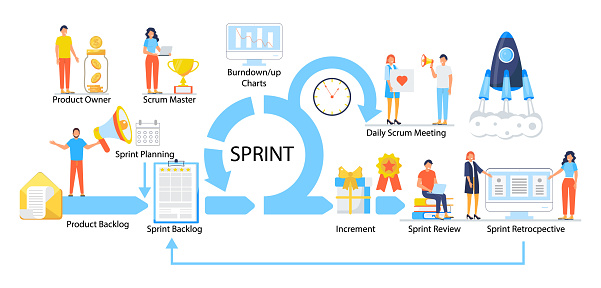
\includegraphics[width=1.0\textwidth]{images/methode-scrum.png}
    \vspace{-1.5cm}
    \caption{La méthode SCRUM}
    \label{fig:methode_scrum}
\end{figure}

\vspace{-0.8cm}

\subsubsection{Pourquoi SCRUM ?}

\vspace{-0.4cm}
Le choix de la méthodologie SCRUM pour le développement du module \textbf{Invoicing} repose sur plusieurs avantages majeurs :

Avec SCRUM, l'équipe de développement bénéficie d'une participation active dans l'évolution du projet. Elle peut s'exprimer librement et s'impliquer dans la prise de décisions, la planification des sprints et l'organisation du travail, contrairement aux méthodes traditionnelles qui figent les spécifications dès le départ et obligent l'équipe à répondre strictement à un cahier des charges initial.

De plus, le fait de présenter des livraisons régulières (incréments) permet de détecter rapidement les éventuelles défaillances, de signaler les blocages et d'ajuster les fonctionnalités selon les besoins réels. Ainsi, le découpage du projet en Sprints rend le travail moins abstrait et facilite la productivité de l'équipe tout au long du cycle de développement.

\vspace{-0.4cm}

\subsubsection{Les principes fondamentaux de SCRUM}

\vspace{-0.3cm}
\begin{itemize}
    \renewcommand{\labelitemi}{\textcolor{royalBlue}{\rule{1.2ex}{1.2ex}}} % Morba3 zre9 sghir
    \setlength{\itemsep}{0.3cm}
    
    \item \textcolor{primaryBlue}{\textbf{Sprints :}} Ce sont des itérations de développement de courte durée, généralement de 2 à 4 semaines, au cours desquelles des fonctionnalités spécifiques sont développées, testées et livrées. Chaque sprint aboutit à un incrément de produit potentiellement livrable.
    
    \vspace{-0.3cm}
    \item \textcolor{primaryBlue}{\textbf{Product Backlog (Backlog du produit) :}} C'est une liste priorisée et évolutive des fonctionnalités à développer. Le \textit{Product Owner} (Responsable produit) est chargé de sa gestion et de sa mise à jour régulière en fonction des nouveaux besoins et des retours des parties prenantes.

    \vspace{-0.3cm}
    \item \textcolor{primaryBlue}{\textbf{Sprint Backlog (Backlog du Sprint) :}} Il s'agit de l'ensemble des éléments du Product Backlog qui ont été sélectionnés pour être réalisés durant le Sprint en cours. C'est le plan de travail de l'équipe de développement.

    \vspace{-0.3cm}
    \item \textcolor{primaryBlue}{\textbf{Daily Scrum (Mêlée quotidienne) :}} Une courte réunion quotidienne (généralement 15 minutes) permettant à l'équipe de développement de se synchroniser, de faire le point sur l'avancement des tâches et d'identifier les blocages éventuels.

    \vspace{-0.3cm}
    \item \textcolor{primaryBlue}{\textbf{Revue et Rétrospective de Sprint :}} À la fin de chaque Sprint, l'équipe présente les fonctionnalités réalisées (incrément) aux parties prenantes lors de la Revue. Ensuite, la Rétrospective permet à l'équipe d'analyser son processus de travail afin de l'améliorer pour les Sprints suivants.
\end{itemize}

\vspace{-0.6cm}

\subsubsection{Équipe du projet}

% --- IMAGE EQUIPE SCRUM ---
\begin{figure}[H]
    \centering
    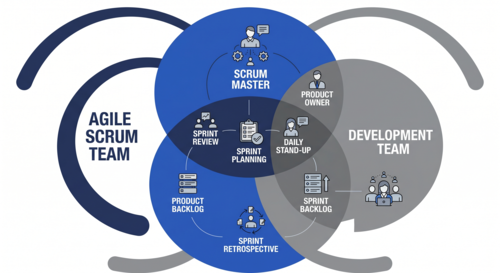
\includegraphics[width=0.80\textwidth]{images/equipe-scrum.png}
    \vspace{-0.4cm}
    \caption{L'équipe SCRUM}
    \label{fig:equipe_scrum}
\end{figure}

\vspace{-0.4cm}
Pour réaliser notre module d'Invoicing, nous avons intégré une équipe constituée de :

\vspace{-0.0cm}

\begin{itemize}
    \renewcommand{\labelitemi}{\textcolor{royalBlue}{\rule{1.2ex}{1.2ex}}} % Morba3 zre9 sghir
    \setlength{\itemsep}{0.3cm}

    \vspace{-0.3cm}
    \item \textcolor{primaryBlue}{\textbf{Scrum Master (Encadrant professionnel) - M. Achraf Saloumi :}} Son rôle est de s'assurer de l'implication de chaque membre, de faciliter le processus Scrum et de nous aider à franchir les différents obstacles que nous pourrions rencontrer.

    \vspace{-0.3cm}
    \item \textcolor{primaryBlue}{\textbf{Architecte Backend - M. Ayoub El Youssoufi :}} Son rôle est de nous superviser dans la conception architecturale et les tâches de la partie backend.

    \vspace{-0.3cm}
    \item \textcolor{primaryBlue}{\textbf{Architecte Frontend - M. El Harraj Abdelatif :}} Son rôle est de nous superviser dans les choix techniques et les tâches de la partie frontend.

    \vspace{-0.3cm}
    \item \textcolor{primaryBlue}{\textbf{Équipe de développement - Redouane Ed-Dahmany, Soufiane Hajji et Mehdi Farhloumi :}} Notre rôle consiste à concevoir, développer et tester les différentes fonctionnalités du projet.
\end{itemize}

\vspace{0.0cm}

\subsubsection{Gestion de projet avec JIRA}

\vspace{-0.4cm}
Comme la méthodologie de travail Scrum que nous utilisons est une approche Agile, l'outil \textbf{JIRA} s'est imposé comme la solution idéale pour gérer et suivre l'avancement de notre projet.

Avec JIRA, une plateforme incontournable de gestion de projets, nous pouvons suivre les différentes étapes du cycle de développement, y compris la spécification du backlog et la planification des sprints.

\vspace{-0.1cm}

% --- IMAGE JIRA ---
\begin{figure}[H]
    \centering
    
\includegraphics[width=0.25\textwidth]{images/jira-gestion.png}
    \vspace{-0.4cm}
    \caption{Interface de gestion de projet JIRA}
    \label{fig:jira_gestion}
\end{figure}

\vspace{-0.4cm}

Voici comment cet outil est appliqué dans notre contexte :

\vspace{-0.1cm}
\noindent\textcolor{primaryBlue}{\textbf{\textit{Spécification du backlog :}}}
\begin{itemize}
    \renewcommand{\labelitemi}{\textcolor{royalBlue}{\textbullet}}
    \setlength{\itemsep}{0.2cm}
    \vspace{-0.1cm}
    \item Utilisation des fonctionnalités de gestion des tâches et des User Stories de JIRA pour définir le backlog du projet.
    \vspace{-0.3cm}
    \item Classement des fonctionnalités par ordre de priorité selon la valeur métier apportée.
\end{itemize}

\vspace{-0.1cm}
\noindent\textcolor{primaryBlue}{\textbf{\textit{Sprint planning :}}}
\begin{itemize}
    \renewcommand{\labelitemi}{\textcolor{royalBlue}{\textbullet}}
    \setlength{\itemsep}{0.2cm}
    \vspace{-0.1cm}
    \item JIRA est utilisé pour visualiser le backlog global et sélectionner les User Stories qui doivent obligatoirement être réalisées pendant le Sprint en cours.
    \vspace{-0.3cm}
    \item Le Scrum Master et l'équipe valident les développements nécessaires pour atteindre l'objectif du Sprint.
\end{itemize}

\vspace{-0.1cm}
\noindent\textcolor{primaryBlue}{\textbf{\textit{Estimation des tâches :}}}
\begin{itemize}
    \renewcommand{\labelitemi}{\textcolor{royalBlue}{\textbullet}}
    \setlength{\itemsep}{0.2cm}
    \vspace{-0.1cm}
    \item Au début de chaque Sprint, une réunion de planification est organisée avec l'équipe de développement pour estimer la complexité des tâches et établir le Sprint Planning.
    \vspace{-0.3cm}
    \item L'équipe de développement estime les tâches à réaliser pendant le sprint en utilisant des points de complexité (Story Points) ou d'effort.
    \vspace{-0.3cm}
    \item Les tâches sont ensuite assignées aux différents membres de l'équipe de développement en utilisant les fonctionnalités de gestion et d'attribution de JIRA.
\end{itemize}

\vspace{-0.1cm}
\noindent\textcolor{primaryBlue}{\textbf{\textit{Suivi du sprint :}}}
\begin{itemize}
    \renewcommand{\labelitemi}{\textcolor{royalBlue}{\textbullet}}
    \setlength{\itemsep}{0.2cm}
    \vspace{-0.1cm}
    \item Une fois le Sprint lancé, le tableau de bord JIRA (Scrum Board) est utilisé pour suivre visuellement l'avancement des tâches en temps réel.
    \vspace{-0.3cm}
    \item Les développeurs peuvent mettre à jour l'état de leurs tâches en les déplaçant de manière fluide à travers les différentes colonnes (À faire, En cours, En test, Terminé).
\end{itemize}

\vspace{0.0cm}

% --- IMAGE JIRA BOARD ---
\begin{figure}[H]
    \centering
    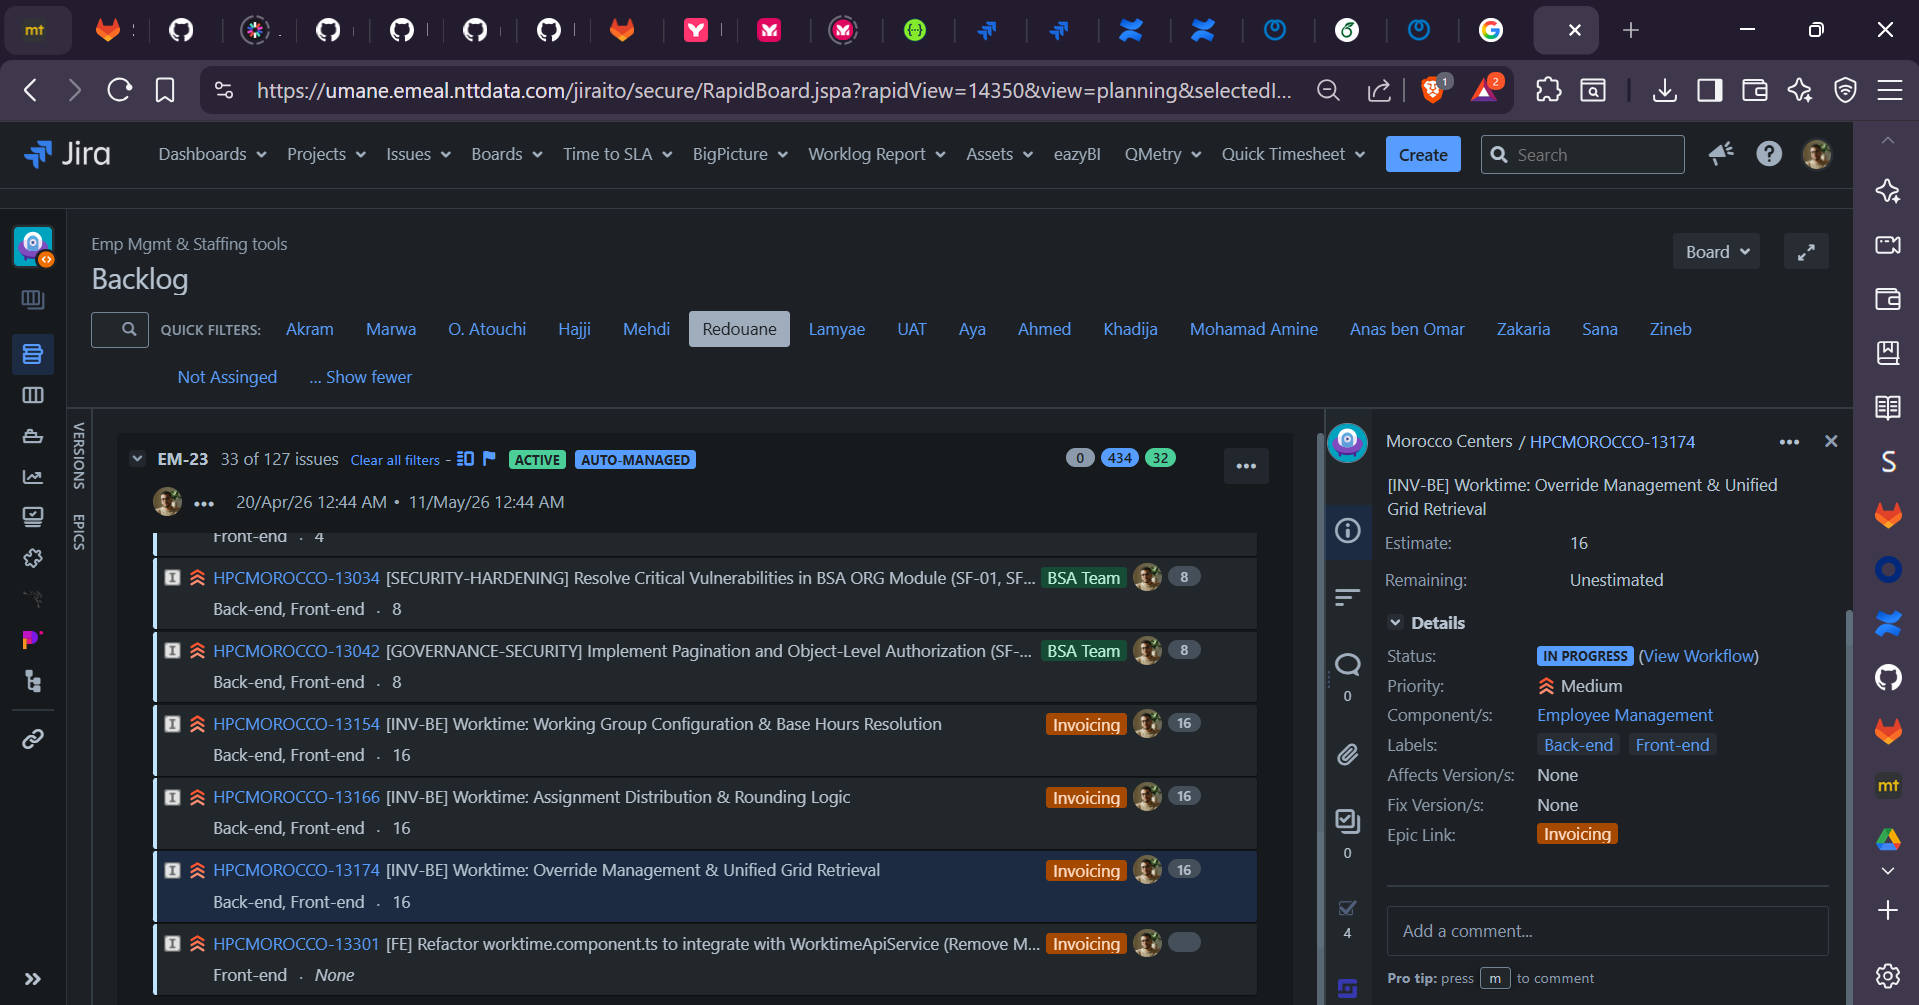
\includegraphics[width=1.0\textwidth]{images/jira-board.png}
    \vspace{-0.8cm}
    \caption{Exemple de suivi de l'avancement des tâches sur JIRA}
    \label{fig:jira_board}
\end{figure}

\vspace{-0.9cm}

\subsubsection{Détail des responsabilités de l'équipe}

\vspace{-0.4cm}
Dans l'optique d'optimiser le cycle de vie du développement et d'assurer une implémentation robuste du module \textbf{Invoicing}, une répartition judicieuse des charges de travail a été instaurée au sein de notre équipe technique. En parfaite adéquation avec notre démarche Agile, l'attribution des périmètres d'intervention — qu'ils soient fonctionnels ou architecturaux — a été pensée de manière à maximiser la synergie du groupe et à garantir une couverture exhaustive des exigences du projet. Le tableau ci-dessous détaille cette affectation des rôles et des missions pour chaque membre :

\vspace{0.4cm}

\begin{table}[H]
    \centering
    \renewcommand{\arraystretch}{1.6} % Tissa3 bin stoura
    \setlength{\arrayrulewidth}{1pt}   % Gheld dyal l-khtouta
    \arrayrulecolor{primaryBlue}       % Loun dyal l-khtouta b zre9

    % Tableau b 3 colonnes m-riglin b l-3bar (\textwidth)
    \begin{tabular}{|>{\centering\arraybackslash}p{0.25\textwidth}|>{\raggedright\arraybackslash}p{0.30\textwidth}|>{\raggedright\arraybackslash}p{0.35\textwidth}|}
        \hline
        % En-tête dyal l'tableau b zre9 mghlo9 w ktba bida
        \rowcolor{primaryBlue}
        \textbf{\textcolor{white}{Membre de l'équipe}} & \textbf{\textcolor{white}{Modules affectés}} & \textbf{\textcolor{white}{Détails des tâches}} \\
        \hline

        % --- REDOUANE (B loun lightBlue) ---
        \rowcolor{lightBlue}
        \textbf{Redouane Ed-Dahmany}\newline \textit{(Moi-même)} & 
        \textbf{Backend :} Worktime, Billing, Export PDF\newline 
        \textbf{Frontend :} UI Admin, Settings, Massive Edit & 
        \textbullet~ Développement backend de la gestion du Worktime.\newline
        \textbullet~ Implémentation de la logique de facturation (Billing).\newline
        \textbullet~ Développement de la génération des factures en PDF.\newline
        \textbullet~ Création des interfaces d'administration.\newline
        \textbullet~ Conception de la vue de modification massive.\newline
        \textbullet~ Intégration des APIs REST côté Angular. \\
        \hline

        % --- SOUFIANE (Bla loun bach yji dakchi m-khalef) ---
        \textbf{Soufiane Hajji} & 
        \textbf{Backend :} Analyse UML, BDD, Service CRUD, Group Mgmt, Ajustements, Sécurité & 
        \textbullet~ Modélisation UML et conception de la base de données.\newline
        \textbullet~ Développement des services CRUD et des groupes.\newline
        \textbullet~ Implémentation de la logique des ajustements (Overrides).\newline
        \textbullet~ Configuration de la sécurité (Spring Security \& JWT).\newline
        \textbullet~ Écriture des tests unitaires backend. \\
        \hline

        % --- MEHDI (B loun lightBlue) ---
        \rowcolor{lightBlue}
        \textbf{Mehdi Farhloumi} & 
        \textbf{Frontend :} Generate, Confirm \& Close Service, UI/UX, Routage & 
        \textbullet~ Frontend de génération et clôture des services.\newline
        \textbullet~ Consommation des APIs REST via les services Angular.\newline
        \textbullet~ Gestion et validation des formulaires (Reactive Forms).\newline
        \textbullet~ Mise en place du routage et protection (Auth Guards).\newline
        \textbullet~ Amélioration de l'expérience utilisateur (UI/UX). \\
        \hline
    \end{tabular}
    \vspace{0.2cm}
    \caption{Détail approfondi des modules et tâches par membre de l'équipe}
    \label{tab:responsabilites_equipe_detail}
\end{table}

Grâce à cette répartition des tâches, chaque membre de l'équipe a pu se concentrer sur des aspects spécifiques du projet, en travaillant de manière collaborative pour assurer la réalisation efficace de chaque module. L'implication de l'équipe de développement dans ces domaines clés garantit un développement robuste et une meilleure expérience utilisateur tout au long du processus de gestion de la facturation et du suivi des temps de travail.

\vspace{-0.4cm}

\subsubsection{Organisation et communication (Microsoft Teams)}

\vspace{-0.4cm}
Dans le cadre de l'organisation de notre projet et pour maintenir une synchronisation parfaite, nous avons adopté \textbf{Microsoft Teams} comme outil principal pour nos réunions quotidiennes et notre communication continue. 

Microsoft Teams est une plateforme de communication et de collaboration en ligne qui offre diverses fonctionnalités pour faciliter les échanges, la coordination et le suivi de l'avancement au sein de l'équipe de travail.

\vspace{-0.0cm}

% --- IMAGE TEAMS F L-WSSET ---
\begin{figure}[H]
    \centering
    
\includegraphics[width=0.12\textwidth]{images/microsoft-teams.png}
    \vspace{-0.4cm}
    \caption{Plateforme de communication Microsoft Teams}
    \label{fig:ms_teams}
\end{figure}

\vspace{-0.4cm}

Les réunions quotidiennes (\textit{Daily Scrum}) sont un élément essentiel de la gestion de projet Agile, car elles permettent de mettre à jour l'équipe sur l'avancement des tâches, d'identifier les problèmes éventuels et de prendre des décisions importantes. En utilisant Microsoft Teams, nous avons pu organiser facilement ces réunions virtuelles, garantissant ainsi une fluidité même lors des séances de télétravail.

\vspace{0.0cm}
Voici quelques-unes des fonctionnalités de Microsoft Teams que nous avons exploitées pour optimiser notre organisation :

\begin{itemize}
    \renewcommand{\labelitemi}{\textcolor{royalBlue}{\rule{1.2ex}{1.2ex}}} % Morba3 zre9 sghir
    \setlength{\itemsep}{0.3cm}

    \vspace{-0.3cm}
    \item \textcolor{primaryBlue}{\textbf{Appels audio et vidéo :}} Nous avons pu effectuer des appels audio ou vidéo avec les membres de l'équipe, ce qui a permis une communication en temps réel et une meilleure compréhension des informations partagées lors des Daily Scrums.

     \vspace{-0.3cm}
    \item \textcolor{primaryBlue}{\textbf{Partage d'écran :}} Nous avons utilisé la fonction de partage d'écran pour présenter des informations, des rapports d'erreurs, des revues de code ou des démonstrations lors de nos réunions. Cela a favorisé une résolution plus rapide des problèmes (Pair programming) et une collaboration plus efficace.

     \vspace{-0.3cm}
    \item \textcolor{primaryBlue}{\textbf{Chat en ligne :}} En dehors des réunions, nous avons utilisé le chat en ligne pour les discussions rapides, les échanges d'informations techniques et les clarifications. Cela a facilité la communication instantanée et a permis de résoudre rapidement les points bloquants.

     \vspace{-0.3cm}
    \item \textcolor{primaryBlue}{\textbf{Gestion des documents :}} Teams offre une intégration native avec l'écosystème Microsoft Office, ce qui nous a permis de partager et de collaborer sur des documents, des diagrammes UML et des spécifications techniques directement dans l'environnement de l'outil. Cela a simplifié le processus de travail et a évité les problèmes liés au contrôle des versions des fichiers.
\end{itemize}

En utilisant Microsoft Teams pour nos réunions quotidiennes, nous avons pu maintenir une communication régulière et efficace au sein de l'équipe, même à distance. Cela nous a permis de rester alignés sur les objectifs du sprint, de résoudre rapidement les problèmes bloquants et de prendre des décisions informées. De plus, l'utilisation de cette plateforme a fortement favorisé la centralisation des informations, des spécifications techniques et des documents, ce qui a simplifié la collaboration et l'organisation globale des tâches liées au module Invoicing.

\vspace{0.0cm}

% --- IMAGE CAPTURE TEAMS ---
\begin{figure}[H]
    \centering
    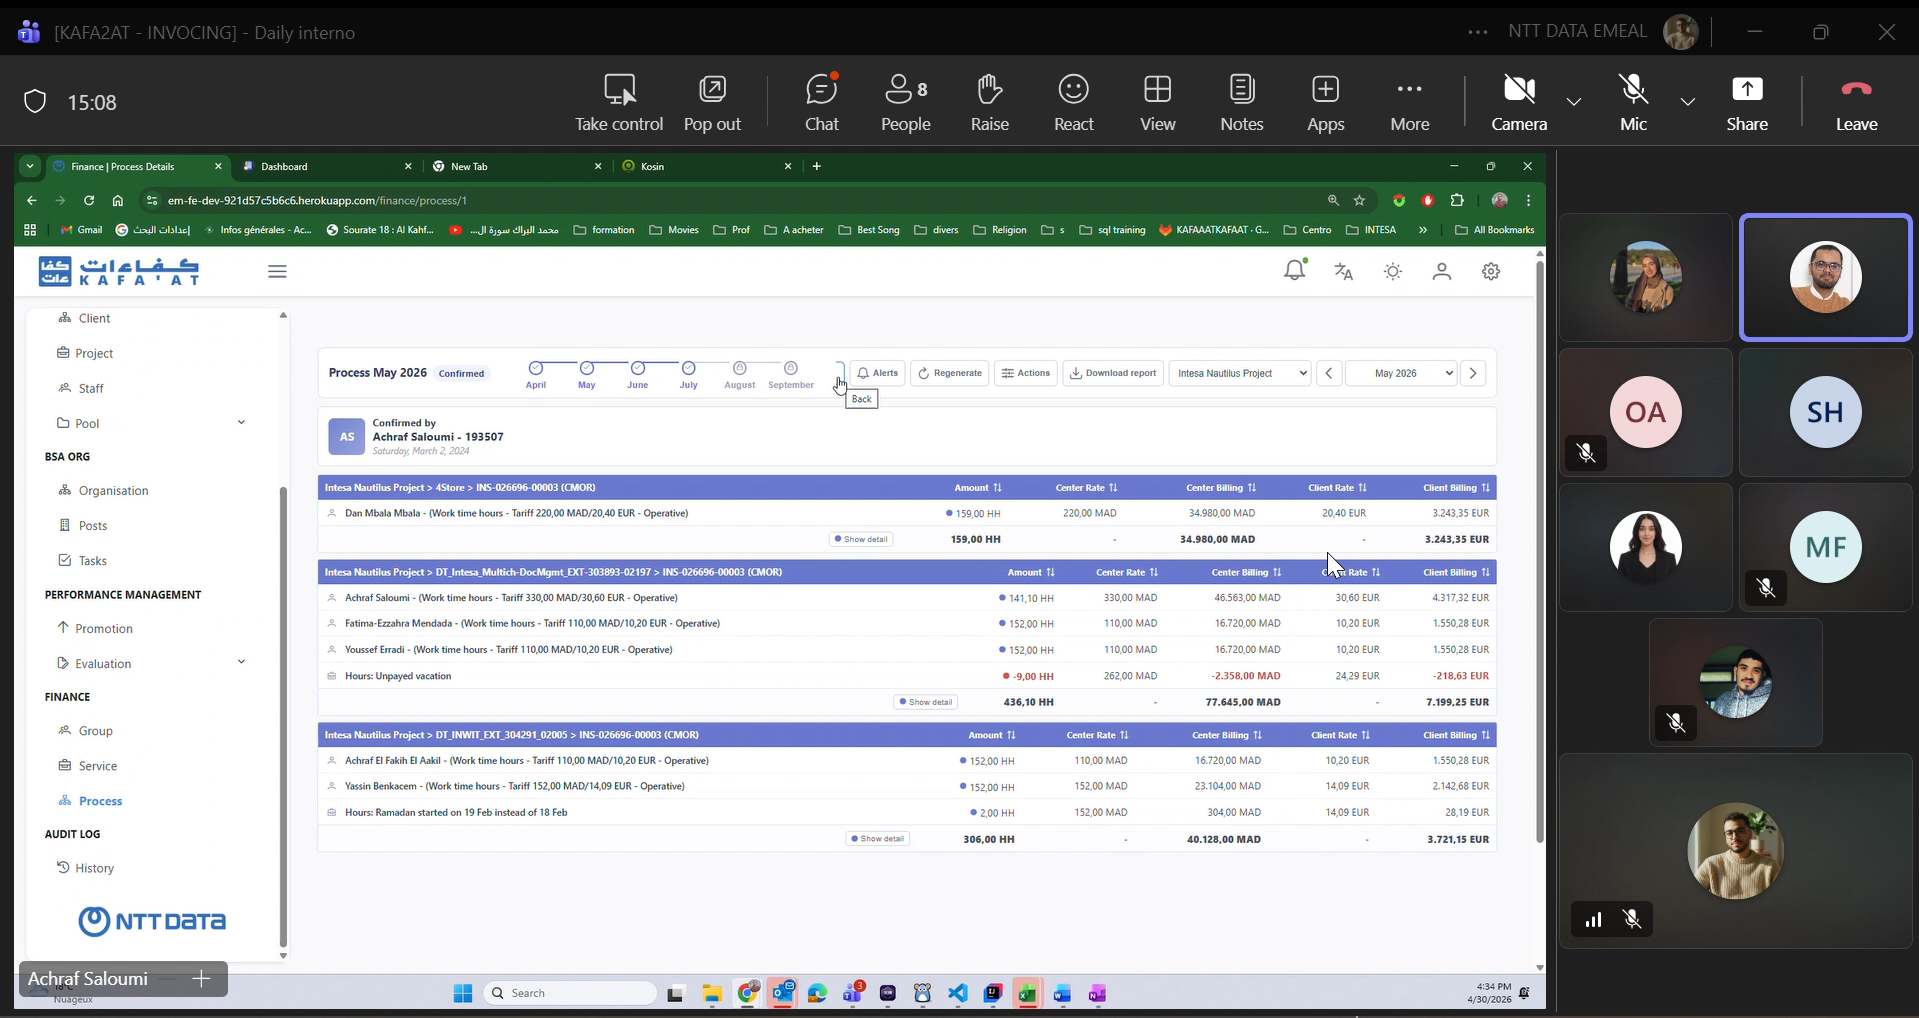
\includegraphics[width=1.0\textwidth]{images/teams-chat.png}
    \vspace{-0.9cm}
    \caption{Collaboration de l'équipe sur Microsoft Teams}
    \label{fig:teams_chat}
\end{figure}

\vspace{-0.7cm}

\subsection{Planification temporelle}

 \vspace{-0.4cm}
La planification du projet est le processus de détermination des objectifs, des activités, des ressources et des délais nécessaires pour atteindre un résultat spécifique dans un projet. Cela implique l'identification des tâches clés, l'estimation des ressources requises, l'établissement d'un calendrier et l'allocation des responsabilités. La planification du projet permet de structurer et d'organiser les différentes étapes du projet, de définir les priorités, d'évaluer les contraintes et de minimiser les risques potentiels. Une planification solide aide à coordonner efficacement les efforts de l'équipe, à optimiser l'utilisation des ressources et à assurer la livraison réussie du projet dans les délais impartis.

\subsubsection{Diagramme de GANTT}

 \vspace{-0.4cm}
Le diagramme de Gantt est un outil de planification et de gestion de projet qui représente visuellement les différentes tâches d'un projet, leur séquence et leur durée. Il est constitué d'une ligne horizontale représentant la période totale du projet, et des barres horizontales qui indiquent le début et la fin de chaque tâche. Les tâches sont organisées en fonction de leur dépendance et de leur ordre logique. [10]

\vspace{-0.0cm}

Le diagramme ci-dessous a été réalisé à l'aide de l'outil de modélisation \textbf{Mermaid} :

\vspace{-0.4cm}

\begin{figure}[H]
    \centering
    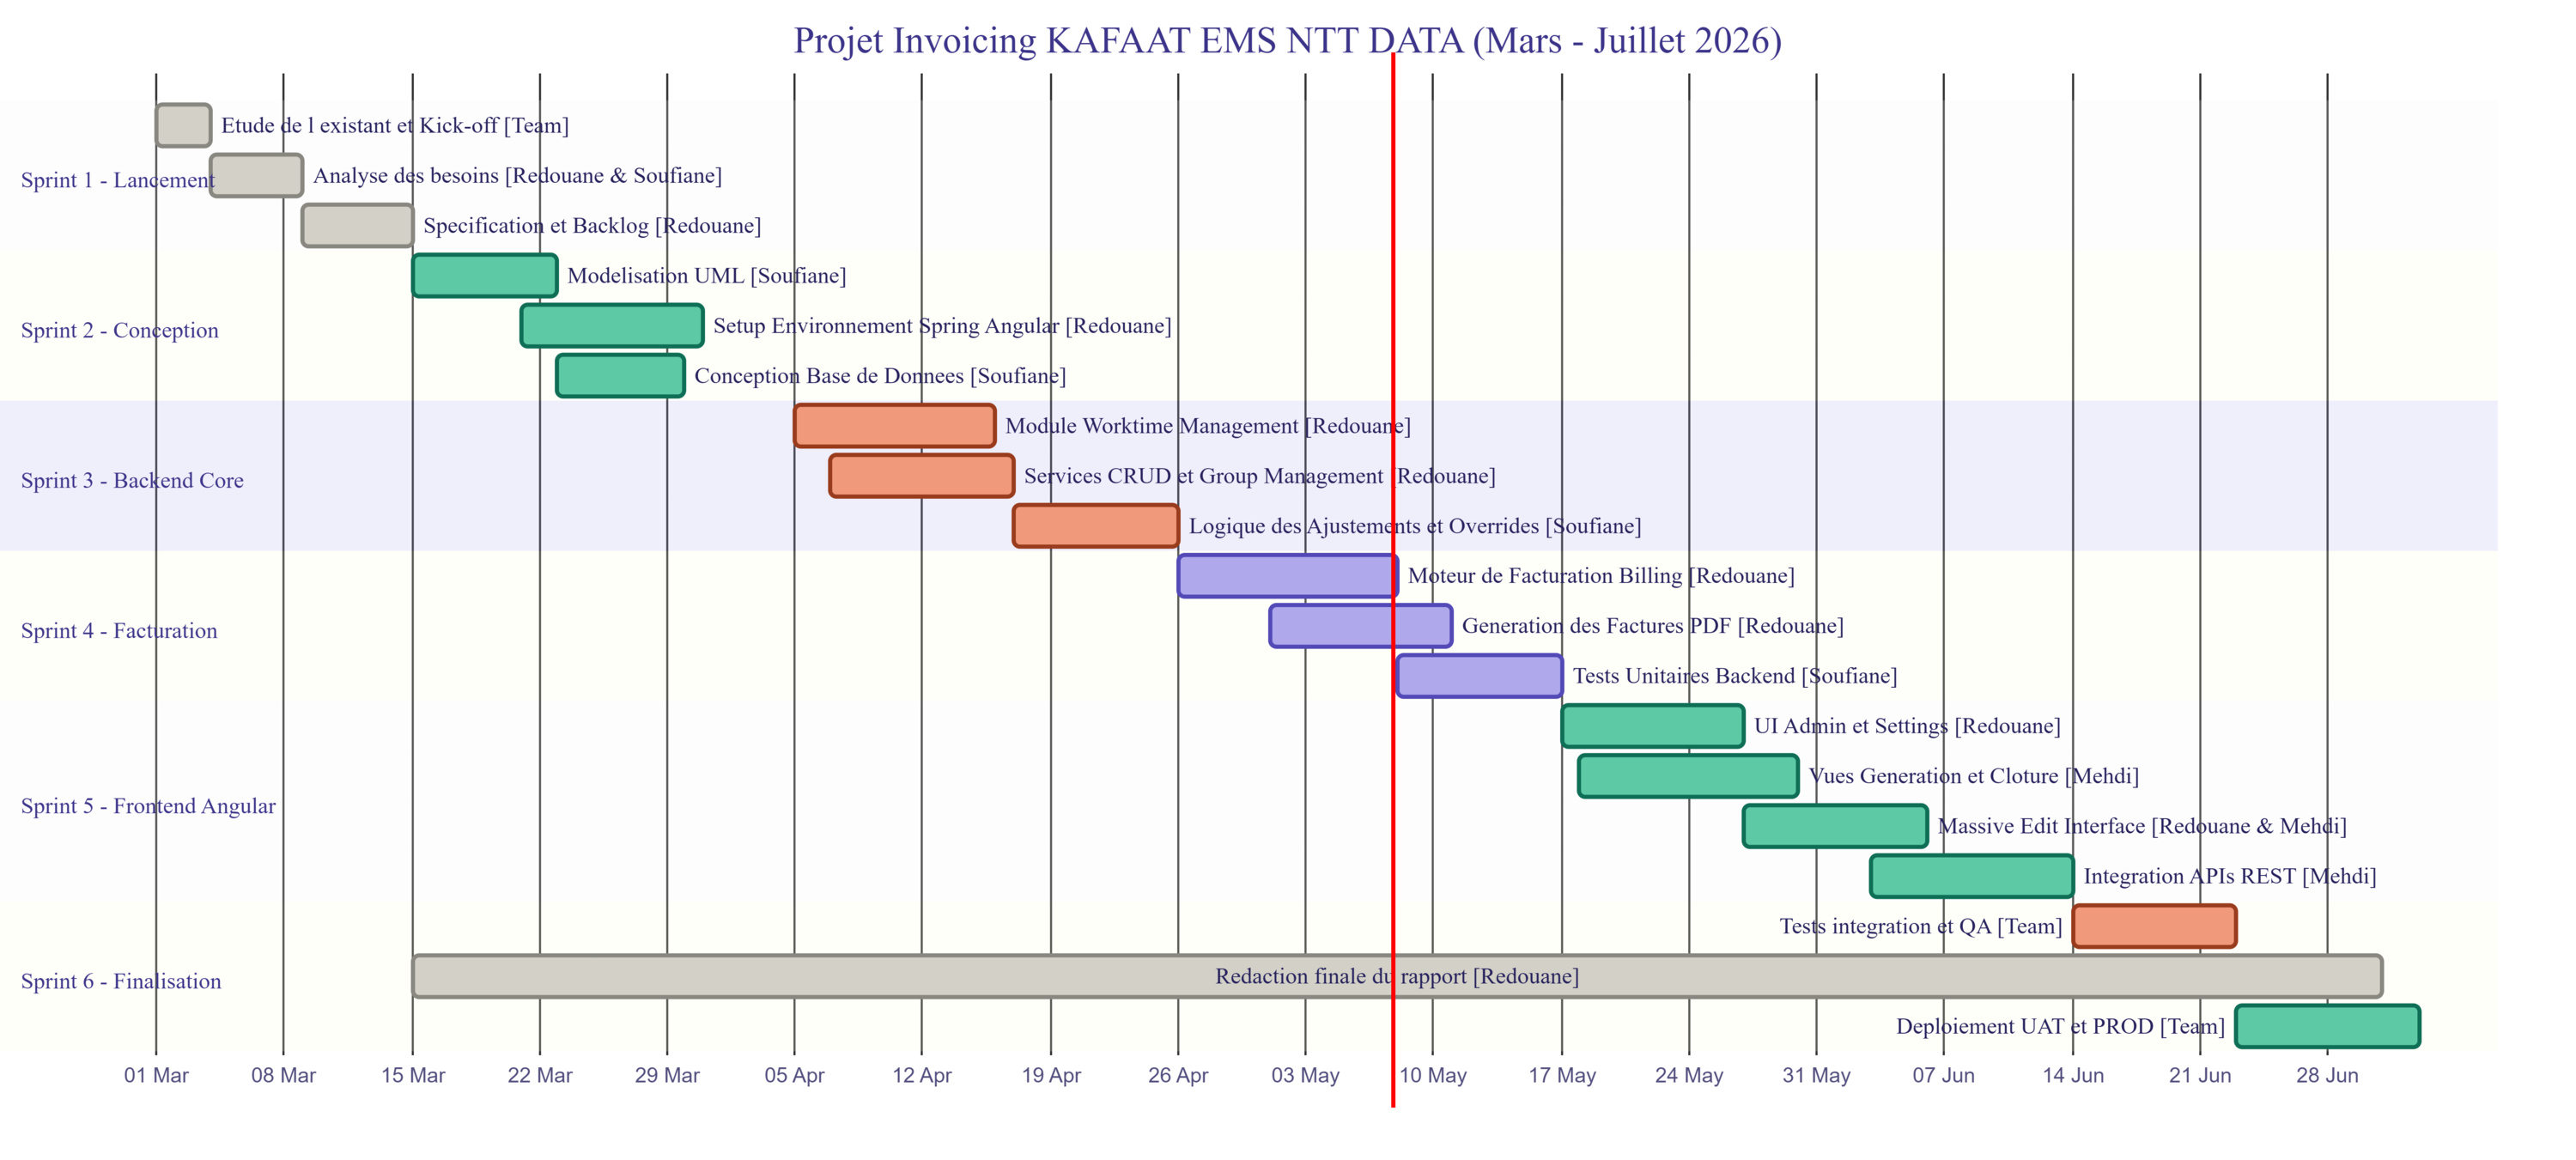
\includegraphics[width=1.0\textwidth]{images/diagramme-gantt-mermaid.png}
    \vspace{-1.2cm}
    \caption{Diagramme de GANTT du projet Invoicing}
    \label{fig:gantt_chart}
\end{figure}

 \vspace{-0.9cm}
\subsubsection{Découpage en Sprints}

 \vspace{-0.4cm}
Le tableau ci-dessous représente la description de chaque sprint, ce qui offre une vision globale de notre travail pendant la durée du stage :

\vspace{0.4cm}

\begin{table}[H]
    \centering
    \renewcommand{\arraystretch}{1.6} 
    \setlength{\arrayrulewidth}{1pt}
    \arrayrulecolor{primaryBlue}

    \begin{tabular}{|>{\raggedright\arraybackslash}p{0.45\textwidth}|>{\centering\arraybackslash}p{0.12\textwidth}|>{\centering\arraybackslash}p{0.15\textwidth}|>{\centering\arraybackslash}p{0.15\textwidth}|}
        \hhline{|-|-|-|-|}
        % En-tête dyal l'tableau
        \rowcolor{primaryBlue}
        \textbf{\textcolor{white}{Activité (Sprint)}} & \textbf{\textcolor{white}{Durée}} & \textbf{\textcolor{white}{Date de début}} & \textbf{\textcolor{white}{Date de fin}} \\
        \hhline{|-|-|-|-|}
        
        % --- SPRINT 1 ---
        \rowcolor{lightBlue}
        \textbf{Sprint 1 : Lancement} \newline
        \textbullet~ Étude de l'existant et Kick-off \newline
        \textbullet~ Analyse des besoins \newline
        \textbullet~ Spécification et Backlog 
        & 14 jours & 01/03/2026 & 14/03/2026 \\
        \hhline{|-|-|-|-|}
        
        % --- SPRINT 2 ---
        \textbf{Sprint 2 : Conception} \newline
        \textbullet~ Modélisation UML \newline
        \textbullet~ Setup Environnement Spring/Angular \newline
        \textbullet~ Conception Base de Données 
        & 16 jours & 15/03/2026 & 30/03/2026 \\
        \hhline{|-|-|-|-|}

        % --- SPRINT 3 ---
        \rowcolor{lightBlue}
        \textbf{Sprint 3 : Backend Core} \newline
        \textbullet~ Module Worktime Management \newline
        \textbullet~ Services CRUD et Group Management \newline
        \textbullet~ Logique des Ajustements et Overrides 
        & 21 jours & 05/04/2026 & 25/04/2026 \\
        \hhline{|-|-|-|-|}

        % --- SPRINT 4 ---
        \textbf{Sprint 4 : Facturation} \newline
        \textbullet~ Moteur de Facturation (Billing) \newline
        \textbullet~ Génération des Factures PDF \newline
        \textbullet~ Tests Unitaires Backend 
        & 21 jours & 26/04/2026 & 16/05/2026 \\
        \hhline{|-|-|-|-|}

        % --- SPRINT 5 ---
        \rowcolor{lightBlue}
        \textbf{Sprint 5 : Frontend Angular} \newline
        \textbullet~ UI Admin et Settings \newline
        \textbullet~ Vues Génération et Clôture \newline
        \textbullet~ Massive Edit Interface \newline
        \textbullet~ Intégration APIs REST 
        & 28 jours & 17/05/2026 & 13/06/2026 \\
        \hhline{|-|-|-|-|}

        % --- SPRINT 6 ---
        \textbf{Sprint 6 : Finalisation} \newline
        \textbullet~ Tests d'intégration et QA \newline
        \textbullet~ Rédaction finale du rapport \newline
        \textbullet~ Déploiement UAT et PROD 
        & 19 jours & 14/06/2026 & 02/07/2026 \\
        \hhline{|-|-|-|-|}
    \end{tabular}
    \caption{Description globale et temporelle des Sprints}
    \label{tab:all_sprints}
\end{table}

\vspace{0.4cm}

\section*{Conclusion}
\addcontentsline{toc}{section}{Conclusion} % Bach t-ban f l'Fihres wakha ma3ndhach ra9m

 \vspace{-0.4cm}
Durant ce premier chapitre, nous avons réussi à fournir une vue d'ensemble du projet en le situant dans son contexte général. Nous avons introduit l'organisme d'accueil, NTT DATA, et nous avons décrit de manière détaillée la problématique à résoudre, ainsi que les objectifs à atteindre dans le cadre du développement du module \textbf{Invoicing} pour la plateforme \textbf{KAFA'AT EMS}.

De plus, nous avons abordé le choix de la méthodologie de travail adoptée (Agile SCRUM) pour assurer la réussite et la flexibilité de réalisation. Nous avons également souligné l'importance de la communication et de la planification pour la gestion efficace des différentes étapes et itérations du projet.

En conclusion, ce premier chapitre nous a permis de poser les fondations du projet en définissant son cadre, ses objectifs et sa méthodologie. Il nous a fourni une compréhension globale du besoin et nous a préparés pour la suite, où nous aborderons les détails spécifiques de l'analyse fonctionnelle et de la conception de notre solution.

% --- CHAPITRE 2 : START ---
\chapterpage{2}{Analyse et Conception}
\chapter{Analyse et Conception}

\vspace*{0.8cm} % <--- ZID HADI HNA BACH TB3ED "INTRODUCTION" 3LA L'KHAT ZRE9

\section*{Introduction}
\addcontentsline{toc}{section}{Introduction} % Bach d-dkhoul l'Fihres

\vspace{-0.4cm}
Dans ce chapitre d'analyse et de conception, nous utiliserons des outils de modélisation tels que les diagrammes UML pour approfondir notre compréhension du projet et détailler l'architecture du module \textbf{Invoicing} au sein de la plateforme \textbf{KAFA'AT EMS}. 

Nous commencerons par décrire les besoins fonctionnels à travers les cas d'utilisation, puis nous concevrons la structure du système à l'aide de diagrammes de classes. Ensuite, nous utiliserons les diagrammes de séquence pour représenter les interactions chronologiques entre les différents acteurs et notre backend Spring Boot. Enfin, les diagrammes d'activité nous aideront à visualiser les flux de travail et les processus de facturation. Ces outils de modélisation nous guideront dans la conception détaillée et la réalisation technique du système.

\vspace{-0.4cm}
\section{Langage UML}

\vspace{-0.5cm}
\subsection{Définition}

\vspace{-0.4cm}
Le langage UML (\textit{Unified Modeling Language}) est un langage de modélisation graphique utilisé pour représenter, spécifier, visualiser et documenter les différents aspects d'un système logiciel. Il fournit un ensemble de notations graphiques standardisées qui permettent aux développeurs, aux architectes et aux analystes de communiquer et de comprendre les concepts, les structures, les comportements et les interactions d'un système.

Le langage UML comprend plusieurs types de diagrammes, tels que les diagrammes de cas d'utilisation, les diagrammes de classes, les diagrammes de séquence, les diagrammes d'activité, et les diagrammes de déploiement. Chaque type de diagramme a une utilisation spécifique et permet de représenter différents aspects du système.

En utilisant UML, les professionnels de l'informatique peuvent modéliser et concevoir des systèmes logiciels de manière claire et précise. Les diagrammes UML servent de documentation visuelle pour décrire l'architecture, les fonctionnalités, les interactions et les dépendances du système, ce qui facilite la compréhension, la communication et la collaboration entre les différentes parties prenantes de notre projet. [11]

\vspace{0.0cm}

\begin{figure}[H]
    \centering
    
\includegraphics[width=0.35\textwidth]{images/uml-logo.png}
    \vspace{-0.4cm}
    \caption{Logo officiel du langage UML}
    \label{fig:uml_logo}
\end{figure}

\vspace{0.0cm}

\subsection{Intérêts de la modélisation UML}

\vspace{-0.4cm}
Le choix du langage UML pour la phase de conception du module \textbf{Invoicing} ne s'est pas fait au hasard. Il s'appuie sur plusieurs atouts majeurs qui répondent directement aux exigences de notre projet :

\vspace{-0.4cm}
% Hna kan-forciw LaTeX y-kheddem morba3 zre9 f ga3 les listes li jayin
\renewcommand{\labelitemi}{{\color{royalBlue}\rule{1.2ex}{1.2ex}}}

\begin{itemize}[leftmargin=*, itemsep=0.3cm]
    \item \textcolor{primaryBlue}{\textbf{Communication :}} UML fournit un langage commun et standardisé. Il a grandement facilité la collaboration et les échanges techniques entre les membres de l'équipe (développeurs et encadrants au sein de NTT DATA) en offrant une vision partagée et claire de l'architecture du système.
    
    \vspace{-0.4cm}
    \item \textcolor{primaryBlue}{\textbf{Modélisation visuelle :}} UML utilise des diagrammes graphiques pour représenter visuellement la structure et le comportement du système. Cela nous a permis de traduire les règles métiers complexes de la facturation en concepts clairs et intuitifs.
    
    \vspace{-0.4cm}
    \item \textcolor{primaryBlue}{\textbf{Abstraction et encapsulation :}} UML favorise une approche orientée objet. Ceci correspond parfaitement aux technologies que nous avons adoptées pour ce projet (\textbf{Java Spring Boot} pour le backend et \textbf{Angular} pour le frontend), facilitant ainsi le passage de la conception au code tout en garantissant une architecture modulaire.
    
    \vspace{-0.4cm}
    \item \textcolor{primaryBlue}{\textbf{Documentation :}} Les diagrammes UML servent de documentation visuelle de référence pour décrire l'architecture, les contraintes et les flux du système. Ils constituent une base solide pour la maintenance et les futures évolutions de la plateforme KAFA'AT EMS.
    
    \vspace{-0.4cm}
    \item \textcolor{primaryBlue}{\textbf{Support d'outils :}} De nombreux outils de modélisation prennent en charge UML (comme Draw.io, PlantUML ou StarUML), ce qui simplifie la création, la modification et l'intégration de ces modèles directement dans notre documentation technique.
\end{itemize}

\vspace{-0.4cm}
En résumé, l'adoption d'UML pour la conception de ce projet nous permet de maîtriser la complexité du module de facturation, d'encapsuler la logique métier et de fournir une documentation claire, tout en bénéficiant d'une transition fluide vers l'implémentation logicielle. [11]

\vspace{-0.6cm}

% --- BDAYA DYAL SECTION 2 : MODELISATION ---

\section{Modélisation du système}

\vspace{-0.7cm}
\subsection{Diagramme de cas d'utilisation}

\vspace{-0.4cm}
Un diagramme de cas d'utilisation est un outil de modélisation dans le langage UML qui représente les interactions entre les acteurs (utilisateurs, systèmes externes ou administrateurs) et un système logiciel. Il permet de capturer les exigences fonctionnelles en décrivant \textit{ce que} le système doit faire, sans pour autant spécifier \textit{comment} il va le faire.

Il permet de visualiser les fonctionnalités du système du point de vue des utilisateurs, en identifiant les différentes actions qu'ils peuvent effectuer et les résultats attendus. Le diagramme de cas d'utilisation est utile pour décrire les exigences fonctionnelles du module \textbf{Invoicing}, définir son périmètre et faciliter la communication entre les parties prenantes. Il aide à comprendre comment les utilisateurs interagissent avec la plateforme KAFA'AT EMS et à concevoir des fonctionnalités centrées sur leurs besoins. [11]

\vspace{-0.5cm}
\subsubsection{Identification des acteurs}

\vspace{-0.4cm}
Dans le cadre de notre module, nous avons identifié deux acteurs principaux : l'administrateur (\textit{Admin}) et l'utilisateur standard (\textit{User} / Employé). L'administrateur possède toutes les fonctionnalités de l'utilisateur, ainsi que des privilèges supplémentaires liés au paramétrage et à la facturation.

L'utilisateur standard peut effectuer diverses actions telles que la consultation de son temps de travail (\textit{Worktime}), la visualisation de ses factures générées, et le suivi de ses données. Ces fonctionnalités permettent à l'utilisateur d'interagir avec le système pour accomplir des tâches spécifiques liées à son profil au sein de NTT DATA.

De son côté, seul l'administrateur a le privilège de configurer les paramètres de facturation, de gérer les groupes d'utilisateurs, d'appliquer des ajustements (\textit{overrides}) et de déclencher le moteur de génération des factures PDF. Ces fonctionnalités critiques sont strictement réservées à l'administrateur, qui possède des droits étendus pour superviser l'ensemble du processus de facturation.

La relation de généralisation entre l'administrateur et l'utilisateur indique que l'administrateur est une catégorie spéciale d'utilisateur qui bénéficie de fonctionnalités et de droits supplémentaires. Cette hiérarchie permet une gestion efficace des autorisations, des rôles et des permissions au sein de notre backend Spring Boot.

En plus de ces deux acteurs humains, nous avons intégré un \textbf{Serveur SMTP (Système Externe)} qui interagit automatiquement avec notre application pour l'envoi des notifications et des factures par courriel aux employés de manière asynchrone.

\vspace{-0.5cm}

\subsubsection{Diagramme de cas d'utilisation général de l'application}

\vspace{-0.4cm}
L'utilisateur (\textit{User} / Employé) peut consulter son tableau de bord, visualiser le suivi de ses temps de travail (\textit{Worktime}), et consulter ou télécharger ses propres factures. Ces actions nécessitent obligatoirement que l'utilisateur s'authentifie au préalable pour pouvoir accéder aux fonctionnalités du système en toute sécurité.

L'administrateur (\textit{Admin}), en plus des fonctionnalités de base disponibles pour l'utilisateur, dispose de privilèges supplémentaires liés au cœur de métier de l'application. Il a la capacité de configurer les paramètres du moteur de facturation (\textit{Billing}), de gérer les groupes d'employés, d'appliquer des ajustements ou des exceptions (\textit{Overrides}) sur les heures enregistrées, et de déclencher la génération et la clôture des factures au format PDF.

En outre, le système fait appel à un acteur externe, le \textbf{Serveur SMTP (Messagerie)}, qui est sollicité automatiquement pour notifier les employés par courriel lors de la génération de leurs factures ou en cas de modifications de leurs pointages.

Il existe une relation de généralisation entre l'administrateur et l'utilisateur, ce qui signifie conceptuellement que l'administrateur est un type spécial d'utilisateur. Il hérite de toutes les actions de l'utilisateur standard tout en bénéficiant de fonctionnalités et de droits d'accès plus étendus pour la gestion de la facturation.

\vspace{-0.1cm}

La figure ci-dessous montre le diagramme général des cas d'utilisation du projet :

\vspace{-0.2cm}

\begin{figure}[H]
    \centering
    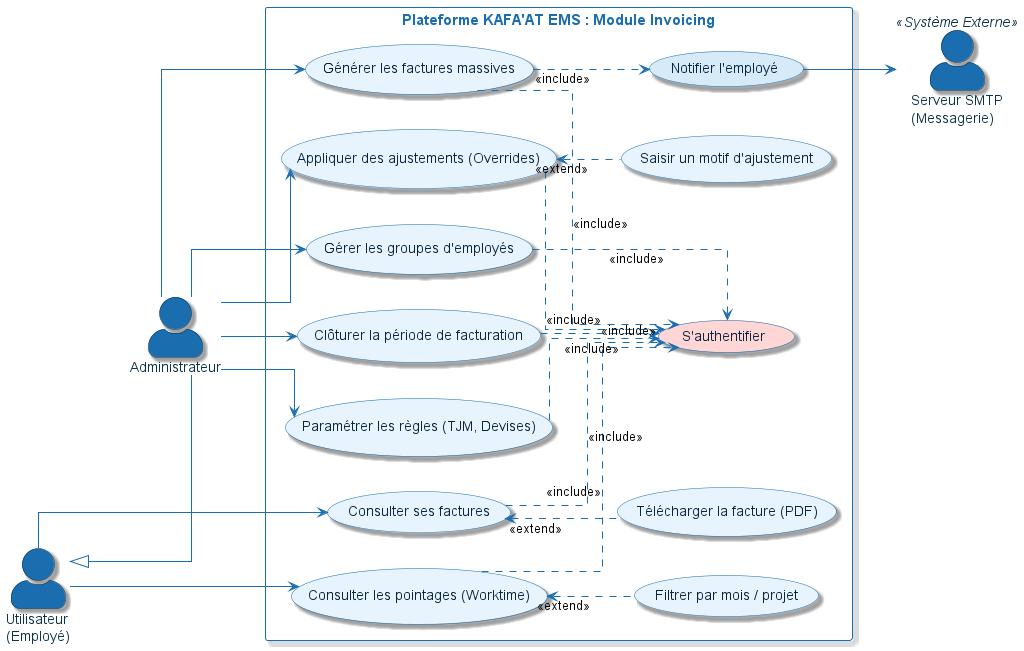
\includegraphics[width=1.0\textwidth]{images/usecase-general.png}
    \vspace{-0.8cm}
    \caption{Diagramme de cas d'utilisation général du module Invoicing}
    \label{fig:usecase_general}
\end{figure}

\vspace{-0.6cm}

\subsubsection{Diagramme de cas d'utilisation de gestion du temps de travail}

\vspace{-0.4cm}
L'utilisateur (\textit{User} / Employé) peut consulter ses propres pointages, soumettre sa feuille de temps, filtrer les pointages existants en fonction de certains critères et exporter le relevé. Pour accéder à ces fonctionnalités, l'utilisateur doit s'authentifier au préalable.

L'administrateur (\textit{Admin}), en plus des fonctionnalités disponibles pour l'utilisateur, possède des privilèges supplémentaires. Il peut consulter les pointages globaux de tous les employés, gérer les jours fériés et les absences, et valider la période mensuelle. De plus, l'administrateur a la possibilité d'appliquer des ajustements (\textit{Overrides}) ou de refuser des pointages. Ces deux actions spécifiques exigent la saisie d'un motif justificatif et déclenchent l'envoi d'une alerte à l'employé via le système externe.

La relation de généralisation entre l'administrateur et l'utilisateur indique que l'administrateur possède toutes les fonctionnalités de l'utilisateur.

\vspace{0.4cm}

La figure ci-dessous montre le diagramme de cas d'utilisation de gestion du temps de travail :

\vspace{0.0cm}

\begin{figure}[H]
    \centering
    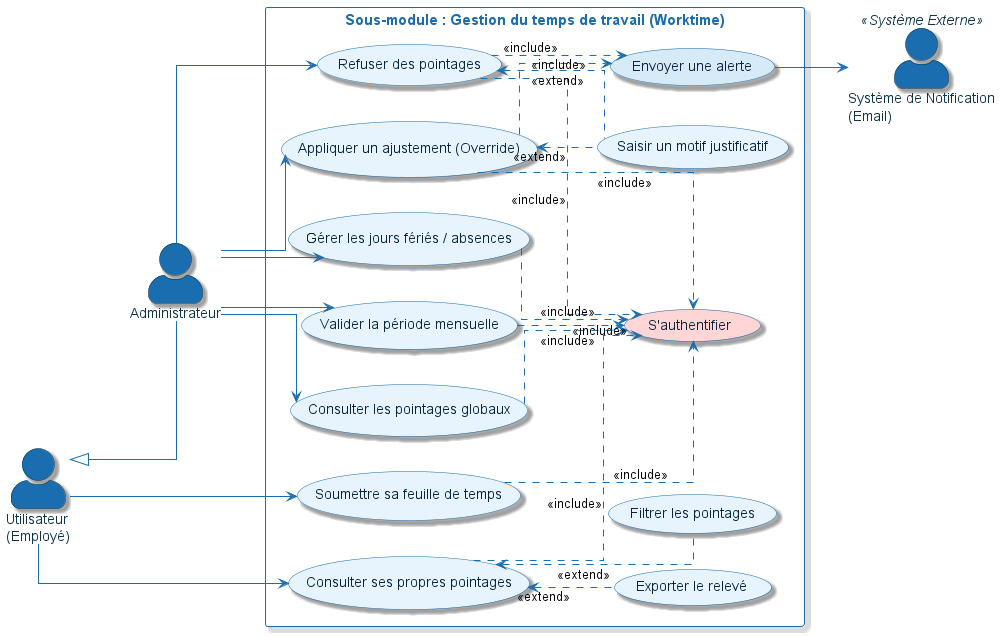
\includegraphics[width=1.0\textwidth]{images/usecase-worktime.png}
    \vspace{-0.8cm}
    \caption{Diagramme de cas d'utilisation de gestion du temps de travail}
    \label{fig:usecase_worktime}
\end{figure}

\vspace{-0.8cm}

\subsubsection{Diagramme de cas d'utilisation de gestion de la facturation}

\vspace{-0.4cm}
L'utilisateur (\textit{User} / Employé) peut consulter l'historique de ses factures et a également la possibilité de télécharger ses factures au format PDF. 

L'administrateur (\textit{Admin}) dispose de fonctionnalités supplémentaires pour gérer le cœur du processus de facturation. Il peut paramétrer les règles de facturation telles que les TJM et les taxes, modifier massivement les factures, lancer la génération massive des factures au format PDF et clôturer la période de facturation. De plus, la génération des factures déclenche automatiquement l'envoi de la facture par email à l'employé via un système de notification externe.

Toutes ces actions nécessitent une authentification préalable pour accéder aux fonctionnalités de gestion de la facturation. La relation de généralisation entre l'administrateur et l'utilisateur indique que l'administrateur possède toutes les fonctionnalités de l'utilisateur.

\vspace{2.4cm}

La figure ci-dessous montre le diagramme de cas d'utilisation de gestion de la facturation :

\vspace{-0.2cm}

\begin{figure}[H]
    \centering
    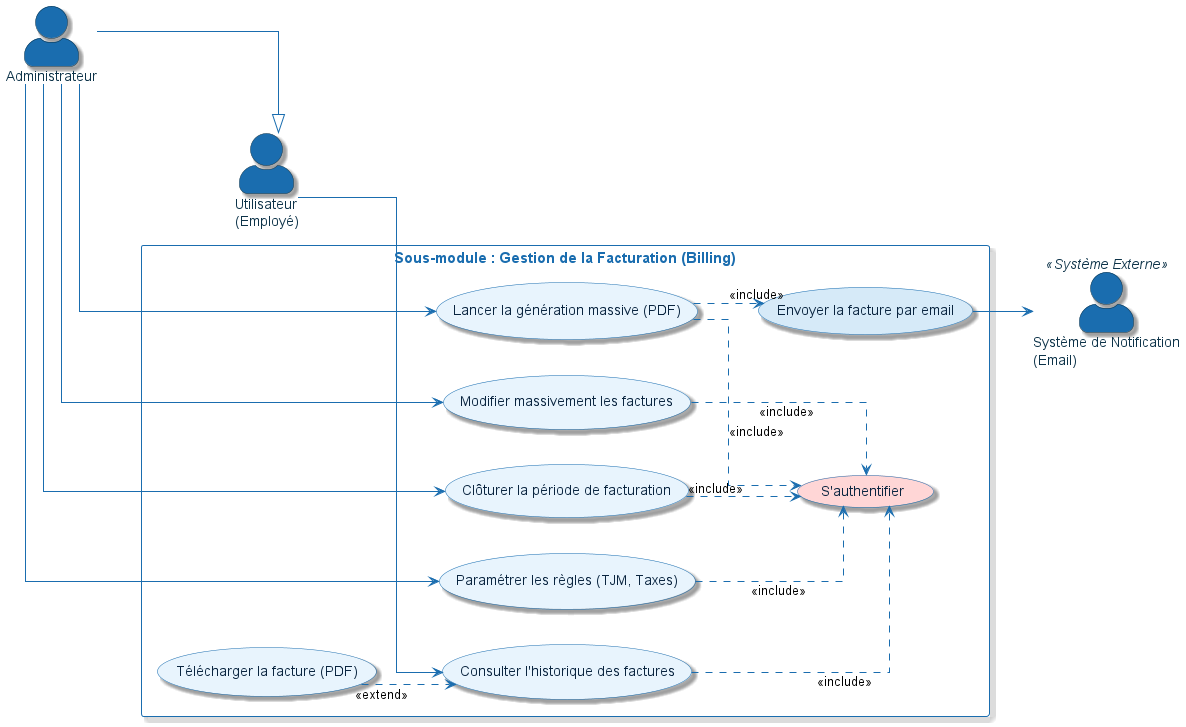
\includegraphics[width=1\textwidth]{images/usecase-billing.png}
    \vspace{-0.9cm}
    \caption{Diagramme de cas d'utilisation de gestion de la facturation}
    \label{fig:usecase_billing}
\end{figure}

\vspace{-0.9cm}

\subsubsection{Diagramme de cas d'utilisation de gestion des groupes et tarification}

\vspace{-0.4cm}
L'utilisateur (\textit{User} / Employé) dispose d'un accès restreint dans cette section. Il a uniquement la possibilité de consulter son propre profil de facturation pour visualiser les modalités qui lui sont appliquées.

L'administrateur (\textit{Admin}) dispose de privilèges supplémentaires, en tant que généralisation de l'utilisateur. Il peut créer un nouveau groupe de facturation (avec la possibilité de définir un plafond d'heures), consulter la liste complète des groupes, modifier un groupe existant, ou encore supprimer un groupe du système. De plus, il a la capacité d'affecter des employés aux différents groupes et de définir le Taux Journalier Moyen (TJM) en spécifiant, si nécessaire, une devise (MAD, EUR, USD). Enfin, l'administrateur peut filtrer la liste des groupes et l'exporter au format Excel.

Toutes ces actions nécessitent une authentification préalable pour accéder aux fonctionnalités de gestion des groupes et de la tarification.

\vspace{2.4cm}

La figure ci-dessous montre le diagramme de cas d'utilisation de gestion des groupes et de la tarification :

\vspace{-0.2cm}

\begin{figure}[H]
    \centering
    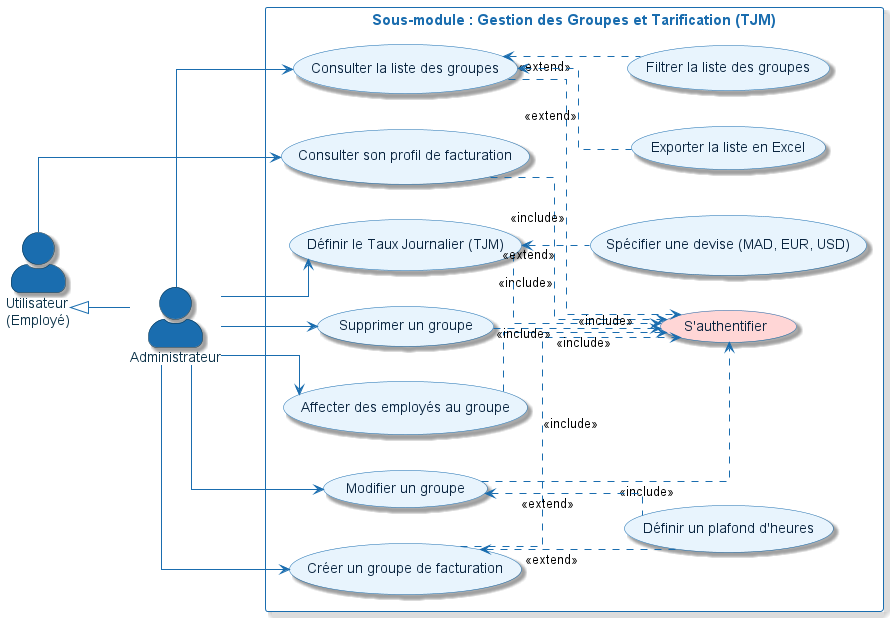
\includegraphics[width=0.95\textwidth]{images/usecase-groupes.png}
    \vspace{-0.4cm}
    \caption{Diagramme de cas d'utilisation de gestion des groupes et tarification}
    \label{fig:usecase_groupes}
\end{figure}

\vspace{-1.0cm}

\subsubsection{Diagramme de cas d'utilisation de gestion des utilisateurs}

\vspace{-0.4cm}
L'utilisateur (\textit{User} / Employé) a la possibilité de consulter son propre profil pour visualiser les informations qui y sont associées. Il peut également mettre à jour ses coordonnées personnelles et changer son mot de passe pour des raisons de sécurité.

L'administrateur (\textit{Admin}) a des fonctionnalités supplémentaires. Il peut consulter la liste complète des employés enregistrés dans le système, créer de nouveaux comptes, et modifier les comptes existants. Lors de la création ou de la modification d'un compte, l'administrateur a la possibilité d'attribuer des rôles spécifiques (privilèges) grâce à un système d'extensions. De plus, il peut réinitialiser le mot de passe d'un utilisateur en cas de besoin. Pour des raisons de traçabilité et d'intégrité des données financières, l'administrateur ne supprime pas définitivement les utilisateurs, mais peut désactiver ou suspendre un compte.

Toutes les actions décrites ci-dessus nécessitent une authentification préalable pour accéder aux fonctionnalités de gestion des utilisateurs. La relation de généralisation entre l'administrateur et l'utilisateur indique que l'administrateur est un type spécial d'utilisateur ayant des privilèges étendus dans le système.

\vspace{0.4cm}

La figure ci-dessous montre le diagramme de cas d'utilisation de gestion des utilisateurs :

\vspace{0.0cm}

\begin{figure}[H]
    \centering
    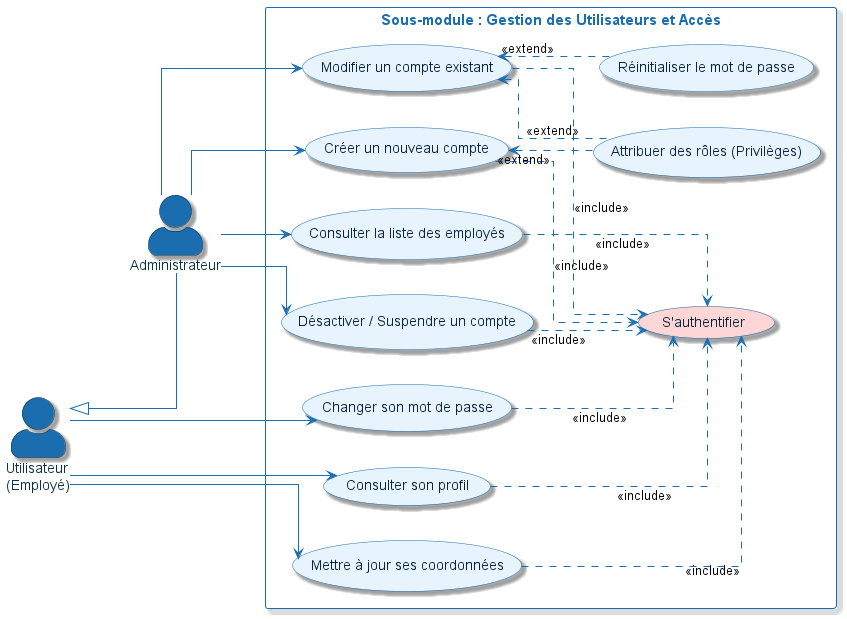
\includegraphics[width=1.0\textwidth]{images/usecase-utilisateurs.png}
    \vspace{-0.8cm}
    \caption{Diagramme de cas d'utilisation de gestion des utilisateurs et des accès}
    \label{fig:usecase_utilisateurs}
\end{figure}

\vspace{-0.8cm}

\subsection{Diagramme de classes}

\vspace{-0.4cm}
Un diagramme de classes est une représentation graphique des classes, des relations entre les classes et des attributs et méthodes associés à chaque classe. Il est utilisé dans le langage de modélisation unifié (UML) pour visualiser la structure statique d'un système logiciel. Le diagramme de classes présente les différentes classes du système et leurs associations, y compris les relations d'héritage, d'agrégation, d'association et de dépendance entre les classes. Il indique également les attributs (variables) et les méthodes (fonctions) définies dans chaque classe. Ce diagramme permet de comprendre la structure du système, les entités impliquées, leurs caractéristiques et leurs interactions. Il facilite la communication entre les développeurs et les concepteurs en fournissant une vue claire et concise de l'architecture logicielle. [11]

Pour répondre aux exigences complexes de la plateforme KAFA'AT EMS (Module Invoicing), notre modélisation s'articule autour de quatre domaines principaux, mis en évidence par un code couleur spécifique :

\begin{itemize}[label=\textcolor{royalBlue}{\rule{1.2ex}{1.2ex}}, leftmargin=*, itemsep=0.2cm]
    \item \textcolor{primaryBlue}{\textbf{Utilisateurs et Sécurité (Bleu foncé) :}} Les classes \texttt{Utilisateur} et \texttt{Administrateur} gèrent l'authentification et les profils. Leurs habilitations sont définies par l'énumération \texttt{Role}.
    \item \textcolor{primaryBlue}{\textbf{Clients et Projets (Bleu moyen) :}} Le système lie le travail à un \texttt{Projet} spécifique, lui-même commandé par un \texttt{Client} (l'entreprise qui sera facturée).
    \item \textcolor{primaryBlue}{\textbf{Gestion du Worktime (Bleu clair) :}} La classe \texttt{Pointage} enregistre les heures déclarées. Son type (Normale, Supp, Férié) est défini par \texttt{TypePointage}. Toute modification effectuée par un administrateur est historisée dans la classe \texttt{Ajustement} pour garantir la traçabilité.
    \item \textcolor{primaryBlue}{\textbf{Moteur de Facturation (Cyan) :}} La classe \texttt{GroupeFacturation} centralise les règles tarifaires (TJM, Devise). Lors de la clôture, le système génère une \texttt{Facture} (liée au Client et à l'Utilisateur) qui est composée de plusieurs \texttt{LigneFacture} détaillant les sous-totaux.
\end{itemize}

\vspace{-0.1cm}

La figure ci-dessous montre le diagramme de classes pour notre projet :

\vspace{-0.2cm}

\begin{figure}[H]
    \centering
    % Dert 1.1\textwidth bach tswira t-ban kbira w y-t9raw les attributs mzyan
    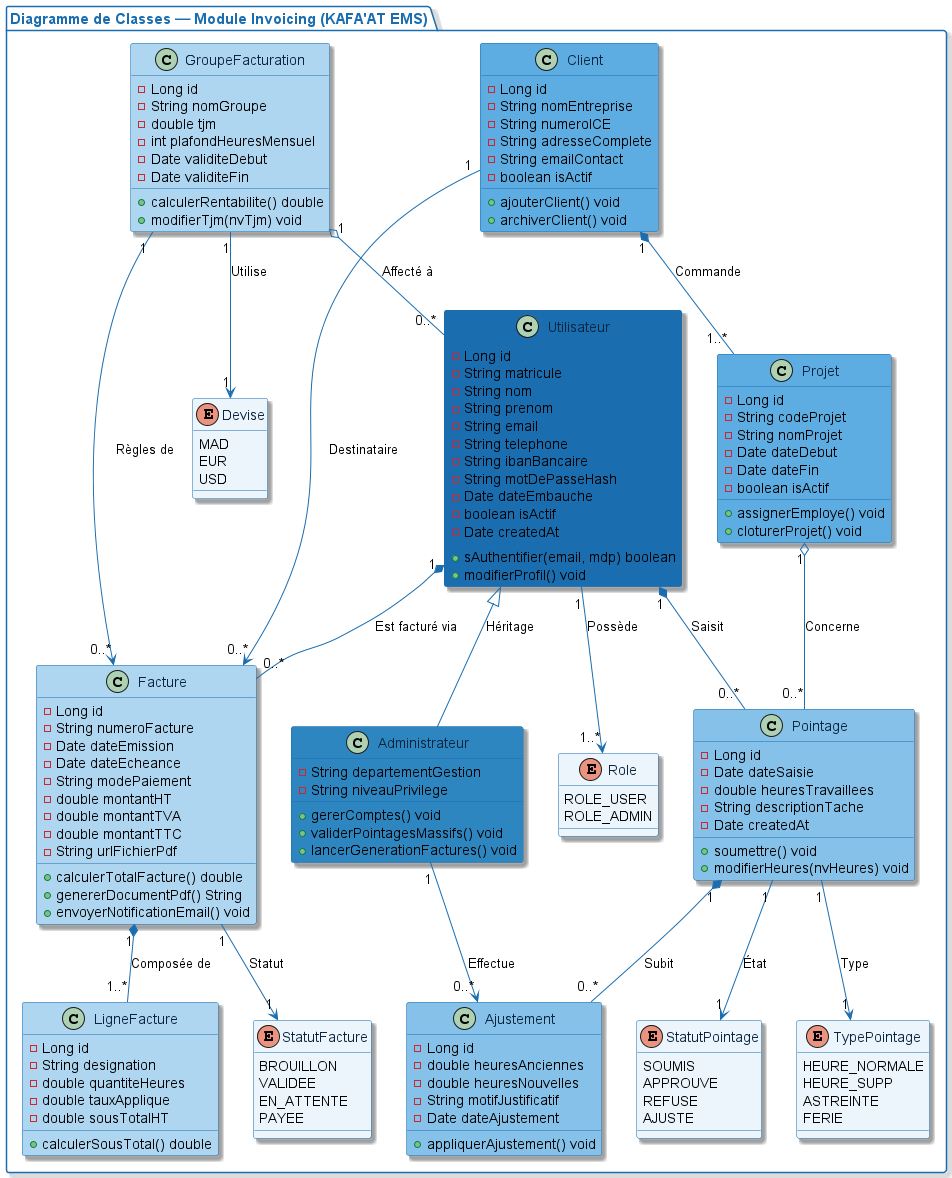
\includegraphics[width=0.92\textwidth]{images/class-diagram.png}
    \vspace{-0.4cm}
    \caption{Diagramme de classes du module Invoicing et Worktime}
    \label{fig:diagramme_classe}
\end{figure}

\vspace{-0.8cm}

\subsection{Diagramme de séquence}

\vspace{-0.4cm}
Un diagramme de séquence est un type de diagramme utilisé dans le langage de modélisation unifié (UML) pour représenter la séquence des interactions entre les objets d'un système. Il met l'accent sur la chronologie des messages échangés entre les objets et les actions qu'ils effectuent en réponse à ces messages. 

Le diagramme de séquence montre l'ordre dans lequel les messages sont envoyés, ainsi que les objets qui envoient et reçoivent ces messages via des "lignes de vie" verticales. Ce diagramme permet de modéliser le comportement dynamique d'un système en montrant comment les composants (Frontend, Backend, Base de données) interagissent pour accomplir un processus métier spécifique. [11]

\vspace{-0.5cm}
\subsubsection{Diagramme de séquence « S'authentifier »}

\vspace{-0.4cm}
L'authentification est une étape cruciale pour sécuriser l'accès à la plateforme KAFA'AT EMS. Notre processus s'appuie sur les standards modernes de sécurité de l'architecture distribuée, notamment \textbf{Spring Security} et les jetons \textbf{JWT (JSON Web Token)}. 



La figure ci-dessous illustre cette séquence d'interactions :

\vspace{-0.3cm}

\begin{figure}[H]
    \centering
    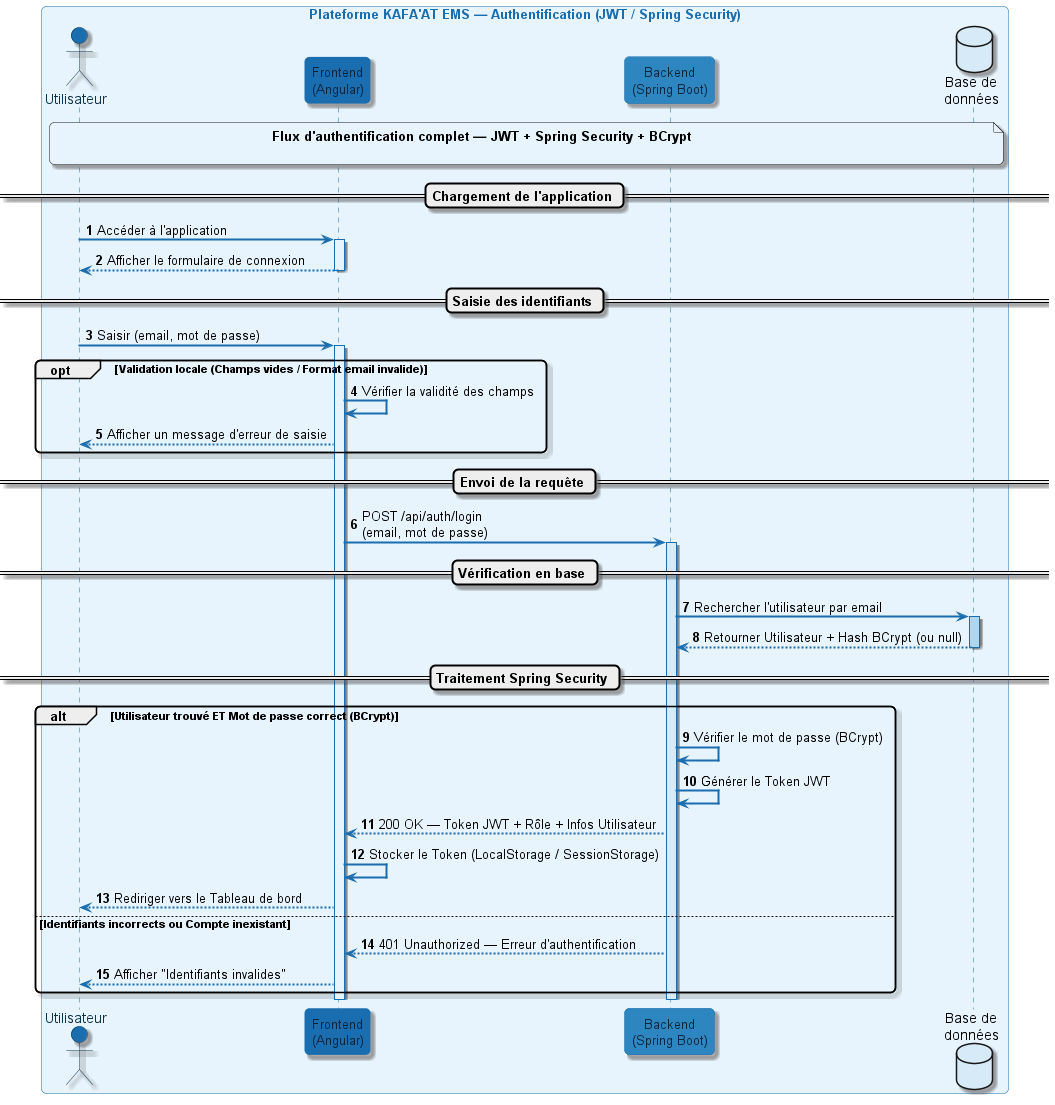
\includegraphics[width=0.92\textwidth]{images/sequence-auth.png}
    \vspace{-0.6cm}
    \caption{Diagramme de séquence d'authentification (JWT \& Spring Security)}
    \label{fig:sequence_auth}
\end{figure}

\vspace{0.0cm}

\subsubsection{Diagramme de séquence « Soumettre un pointage »}

\vspace{-0.4cm}
L'enregistrement du temps de travail (Worktime) est l'une des fonctionnalités centrales pour l'employé. Ce processus n'est pas une simple insertion de données ; il implique une validation métier rigoureuse au niveau du \textbf{Backend (Spring Boot)} pour vérifier que les règles de l'entreprise sont respectées (par exemple, s'assurer que le cumul d'heures saisies pour une même journée ne dépasse pas le plafond autorisé).

La figure ci-dessous détaille les interactions entre le Frontend (Angular), le Backend et la base de données lors de la soumission d'un pointage :

\vspace{-0.3cm}

\begin{figure}[H]
    \centering
    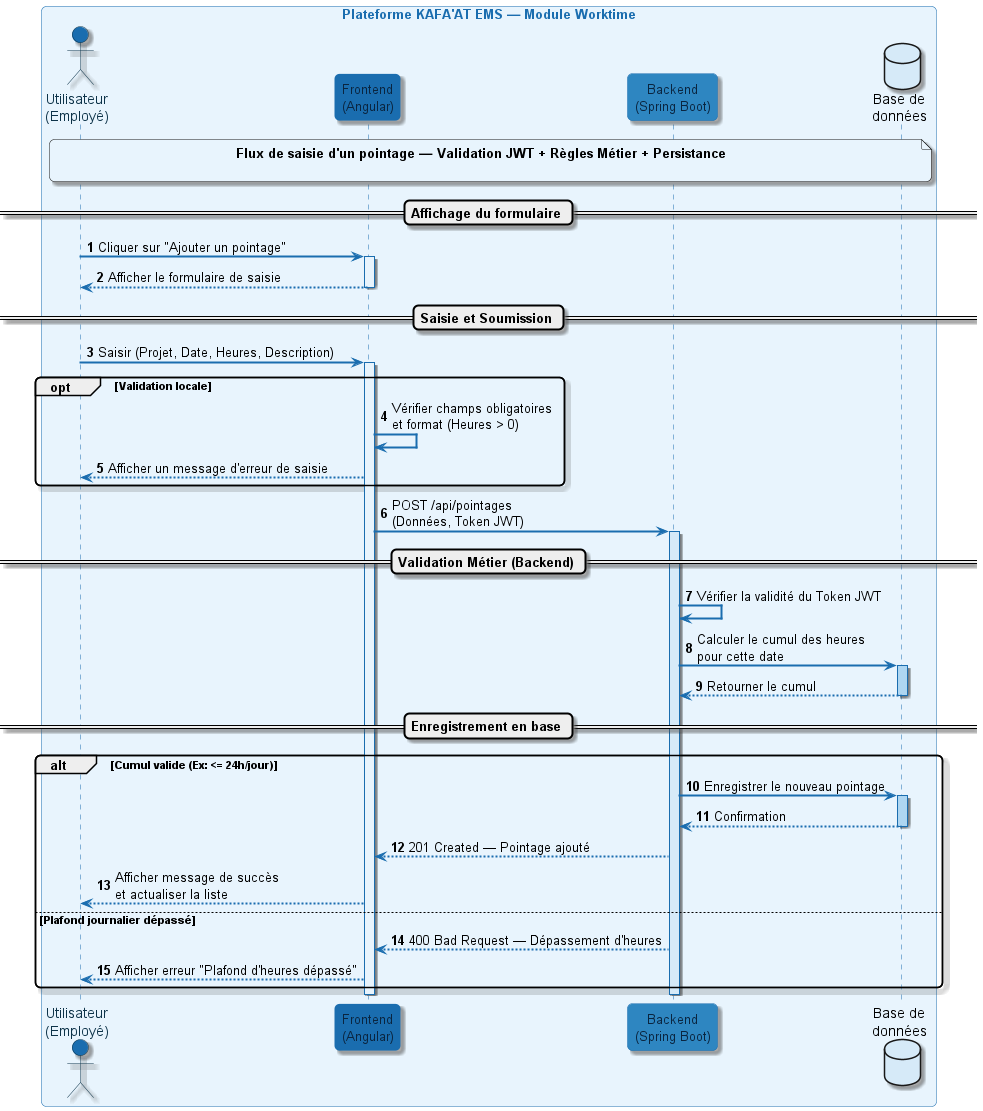
\includegraphics[width=0.92\textwidth]{images/sequence-pointage.png}
    \vspace{-0.4cm}
    \caption{Diagramme de séquence de la soumission d'un pointage}
    \label{fig:sequence_pointage}
\end{figure}

\vspace{0.4cm}

\subsubsection{Diagramme de séquence « Génération massive des factures »}

\vspace{-0.4cm}
Ce diagramme illustre le cœur du processus métier de notre application, une tâche exclusivement réservée à l'administrateur. La génération massive des factures est une opération complexe qui fait intervenir de multiples composants du système.

Lors du déclenchement, le \textbf{Backend (Spring Boot)} vérifie les habilitations, puis interroge la base de données pour récupérer les pointages validés et les taux tarifaires (TJM) associés à chaque groupe d'employés. Le système effectue ensuite les calculs financiers (montants HT, taxes), génère les documents au format \textbf{PDF}, et les sauvegarde en base de données. Enfin, de manière asynchrone pour ne pas bloquer l'interface, le backend communique avec un \textbf{Serveur SMTP externe} pour envoyer automatiquement les factures par courriel aux collaborateurs concernés.

\vspace{0.4cm}

\begin{figure}[H]
    \centering
    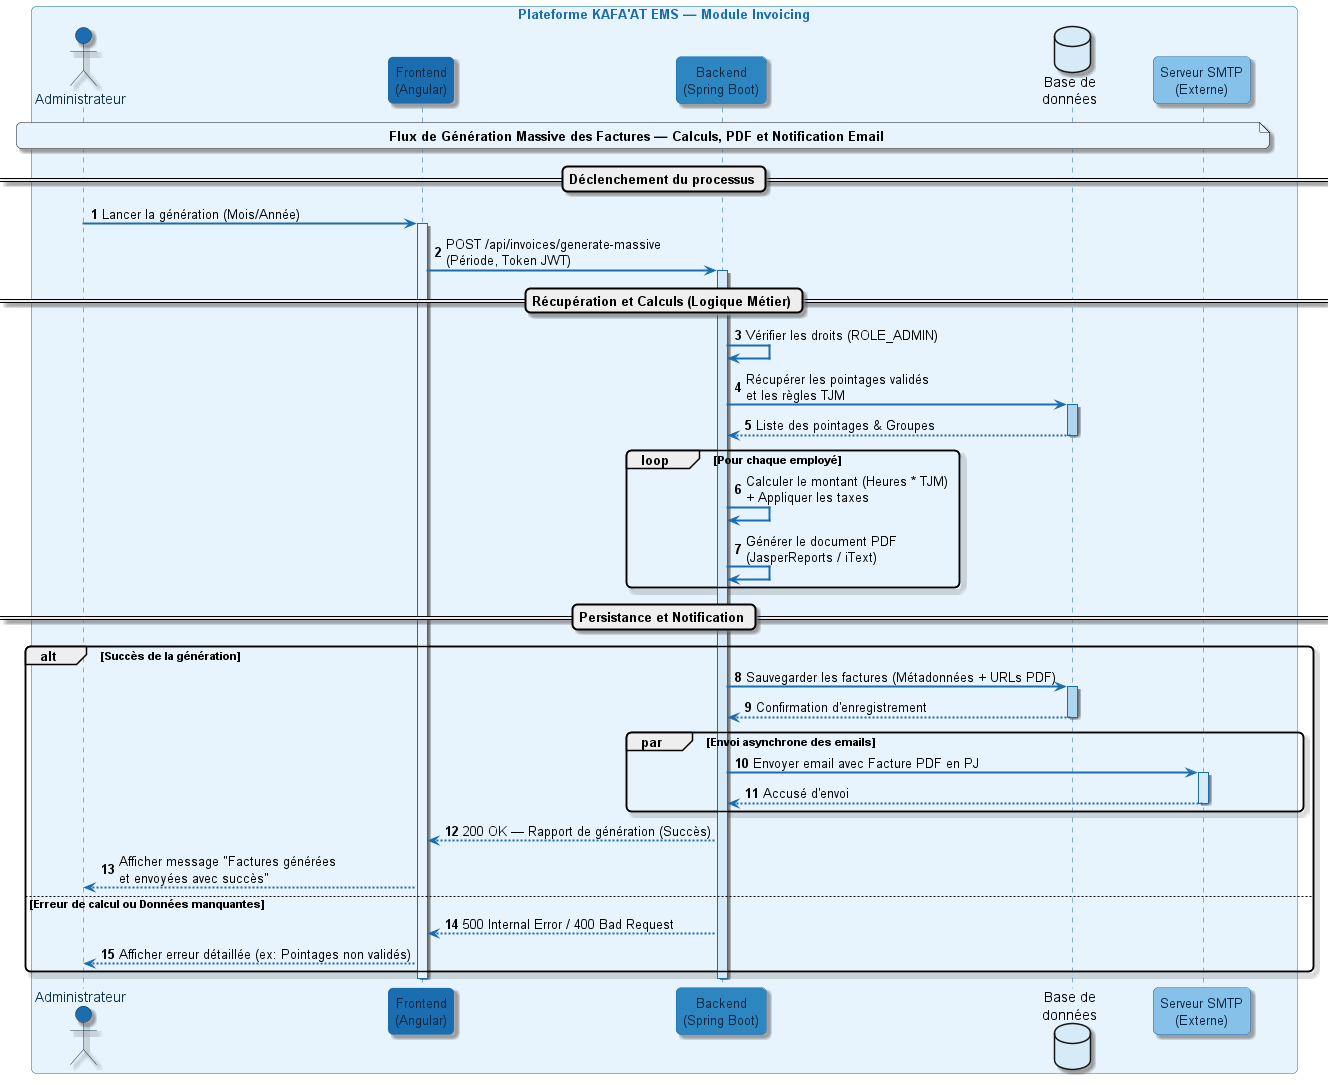
\includegraphics[width=1\textwidth]{images/sequence-facturation.png}
    \vspace{-0.9cm}
    \caption{Diagramme de séquence de la génération massive des factures}
    \label{fig:sequence_facturation}
\end{figure}

\vspace{0.4cm}

\subsubsection{Diagramme de séquence « Désactiver un compte utilisateur »}

\vspace{-0.4cm}
Dans un système de gestion financière et de suivi du temps de travail, la suppression définitive d'un utilisateur (Hard Delete) est proscrite afin de préserver l'intégrité de l'historique des factures et des pointages. Par conséquent, nous avons opté pour un mécanisme de \textbf{Soft Delete} (désactivation logique).

Ce diagramme met en évidence le contrôle d'accès basé sur les rôles (RBAC) mis en place au niveau de Spring Security. Lorsqu'une requête de désactivation est émise, le \textbf{Backend} vérifie impérativement que le jeton JWT transmis contient le rôle \texttt{ROLE\_ADMIN} avant de procéder à la mise à jour du statut du compte (\texttt{isActif = false}) dans la base de données.

\vspace{0.4cm}

\begin{figure}[H]
    \centering
    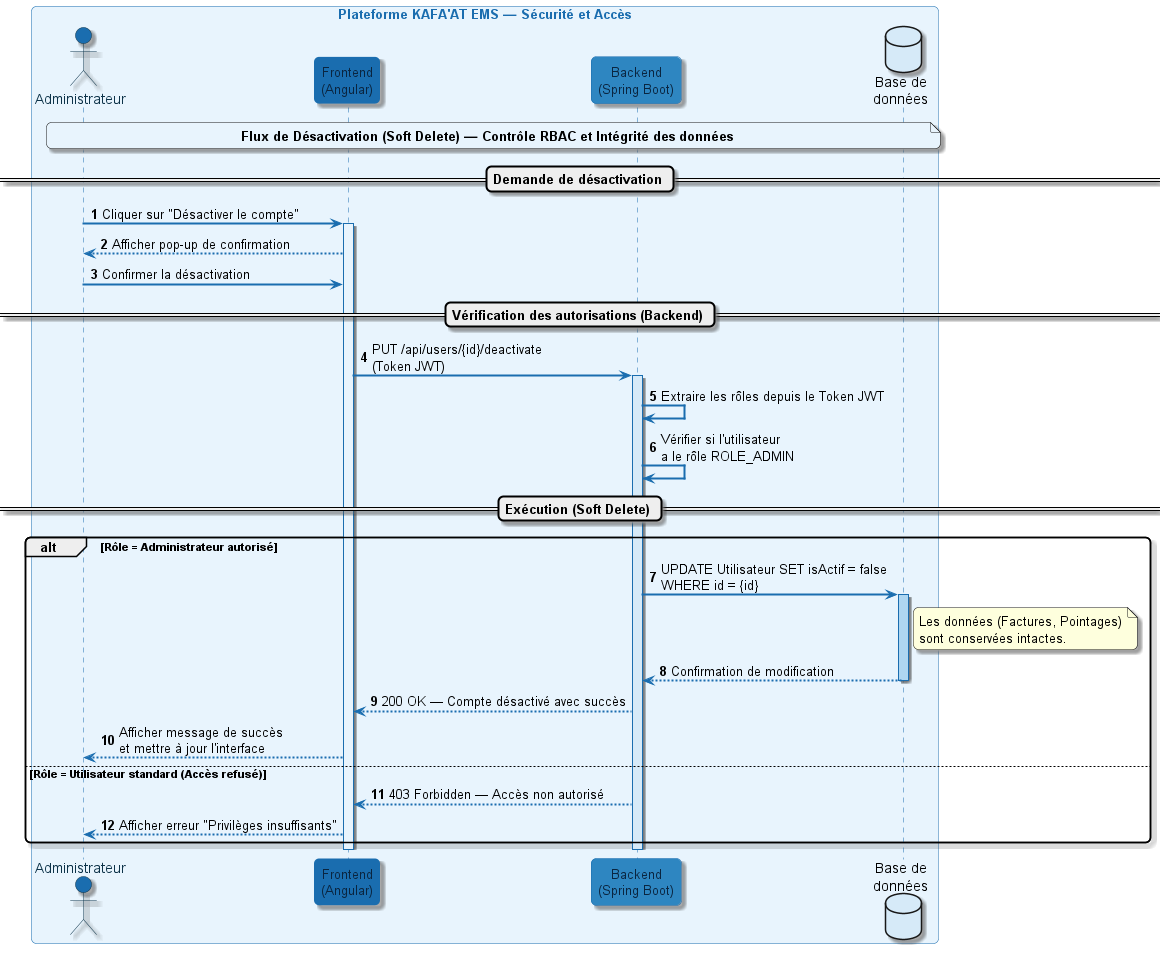
\includegraphics[width=1\textwidth]{images/sequence-desactivation.png}
    \vspace{-0.9cm}
    \caption{Diagramme de séquence de la désactivation d'un compte (Soft Delete)}
    \label{fig:sequence_desactivation}
\end{figure}

\vspace{0.4cm}

\subsubsection{Diagramme de séquence « Créer un groupe de facturation »}

\vspace{-0.4cm}
La configuration des groupes de facturation est un prérequis indispensable pour le fonctionnement du moteur d'invoicing. C'est à travers cette interface que l'administrateur définit les règles de tarification (Taux Journalier Moyen, Devise, Plafond d'heures) qui seront appliquées aux collaborateurs.

Ce diagramme de séquence illustre le processus d'ajout d'un nouveau groupe. Au-delà de la simple insertion de données, le \textbf{Backend} implémente une logique de validation métier pour garantir l'intégrité de la base de données. Il vérifie notamment les privilèges de l'utilisateur (\texttt{ROLE\_ADMIN}) et s'assure qu'aucun groupe portant le même nom n'existe déjà, évitant ainsi les doublons et les conflits financiers (\texttt{409 Conflict}).

\vspace{-0.3cm}

\begin{figure}[H]
    \centering
    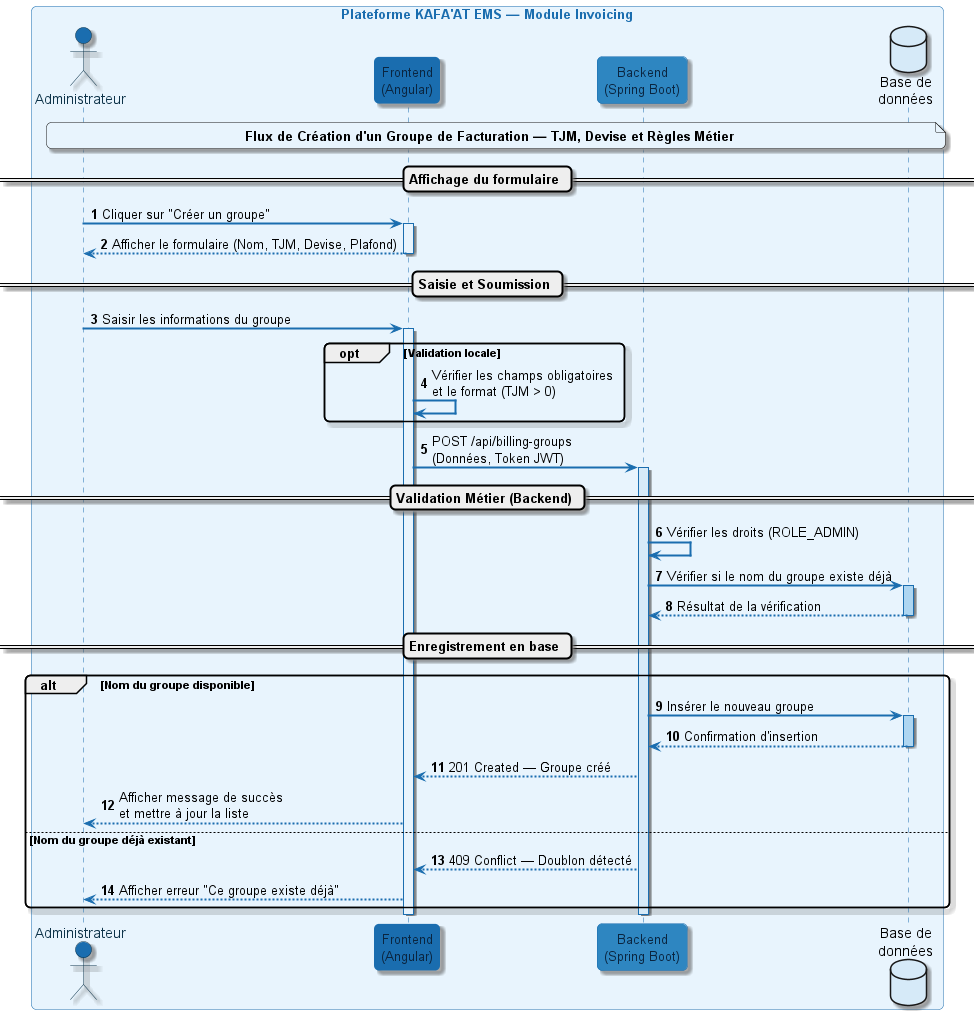
\includegraphics[width=0.92\textwidth]{images/sequence-groupe-facturation.png}
    \vspace{-0.4cm}
    \caption{Diagramme de séquence de la création d'un groupe de facturation}
    \label{fig:sequence_groupe_facturation}
\end{figure}

\vspace{0.4cm}

\subsubsection{Diagramme de séquence « Appliquer un ajustement »}

\vspace{-0.4cm}
Afin de garantir une traçabilité totale et une transparence financière au sein de la plateforme, la modification des heures de travail déclarées par un employé n'est pas une simple mise à jour en base de données. 

Lorsqu'un administrateur constate une anomalie et décide d'appliquer un ajustement (Override) sur un pointage, ce diagramme de séquence montre la rigueur du processus métier implémenté. Le système exige obligatoirement la saisie d'un \textbf{motif justificatif}. Une fois l'ajustement historisé en base de données de manière immuable, le \textbf{Backend} déclenche l'envoi d'une alerte automatique via le \textbf{serveur SMTP} pour notifier l'employé concerné de la modification de sa feuille de temps.

\vspace{-0.1cm}

\begin{figure}[H]
    \centering
    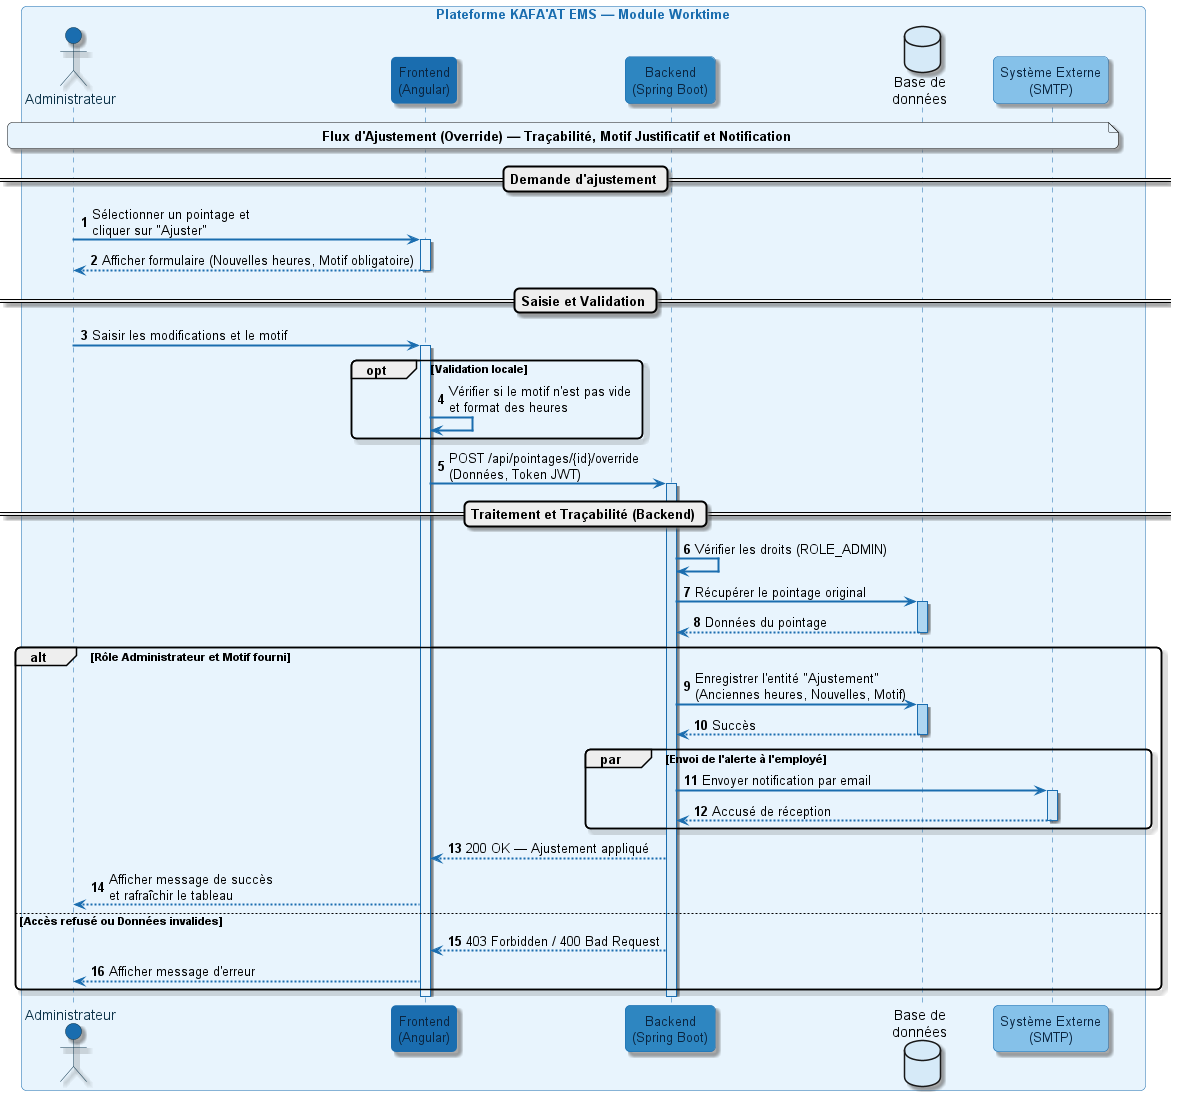
\includegraphics[width=1.0\textwidth]{images/sequence-override.png}
    \vspace{-0.8cm}
    \caption{Diagramme de séquence d'un ajustement de pointage (Override)}
    \label{fig:sequence_override}
\end{figure}

\vspace{0.4cm}

\subsubsection{Diagramme de séquence « Gestion détaillée d'une facture »}

\vspace{-0.4cm}
La gestion d'une facture générée n'est pas une simple opération de mise à jour, mais englobe tout le cycle de vie du document financier. Ce diagramme illustre un scénario complexe où l'administrateur interagit avec plusieurs fonctionnalités liées à une même facture.

Le processus s'amorce par une modification des informations fondamentales de la facture (telle que l'application d'une remise commerciale exceptionnelle, l'ajustement ponctuel du TJM, ou la révision de la date d'échéance). Une fois ces données de base validées et persistées, l'architecture du système, conçue pour être hautement modulaire, prévoit des blocs d'exécution optionnels (\texttt{opt}). Ces blocs offrent à l'administrateur une gestion granulaire du cycle de vie du document financier, lui permettant de :

\begin{itemize}[label=\textcolor{royalBlue}{\rule{1.2ex}{1.2ex}}, leftmargin=*, itemsep=0.2cm]
    \item \textcolor{primaryBlue}{\textbf{Gérer les transitions d'état financier :}} Mettre à jour le statut de la facture (par exemple, la faire passer de \textit{EN\_ATTENTE} à \textit{PAYÉE}) lors de la confirmation du règlement par le client. Cette action est vitale pour la cohérence des tableaux de bord de suivi et permet de verrouiller la facture contre toute modification ultérieure.
    
    \item \textcolor{primaryBlue}{\textbf{Déclencher la régénération dynamique du document :}} Initier la création d'un nouveau document PDF de manière asynchrone. Si les montants, les taxes ou les remises ont été altérés lors de l'étape précédente, le système doit impérativement recalculer les totaux et écraser l'ancienne version. Cela garantit une stricte conformité entre les données relationnelles (Base de données) et le document physique archivé.
    
    \item \textcolor{primaryBlue}{\textbf{Assurer une récupération sécurisée du fichier :}} Interroger l'API du serveur pour télécharger le fichier PDF final. Le Backend, après avoir vérifié les habilitations via le Token JWT, renvoie le fichier sous forme de flux binaire (\textit{Blob}). Cette approche optimise la consommation de la bande passante et sécurise l'accès aux documents sensibles en évitant l'exposition d'URL publiques statiques.
\end{itemize}

\vspace{0.4cm}

\begin{figure}[H]
    \centering
    % Drt 1.05\textwidth bach y-ban l-code li wset les 'opt' waaaade7
    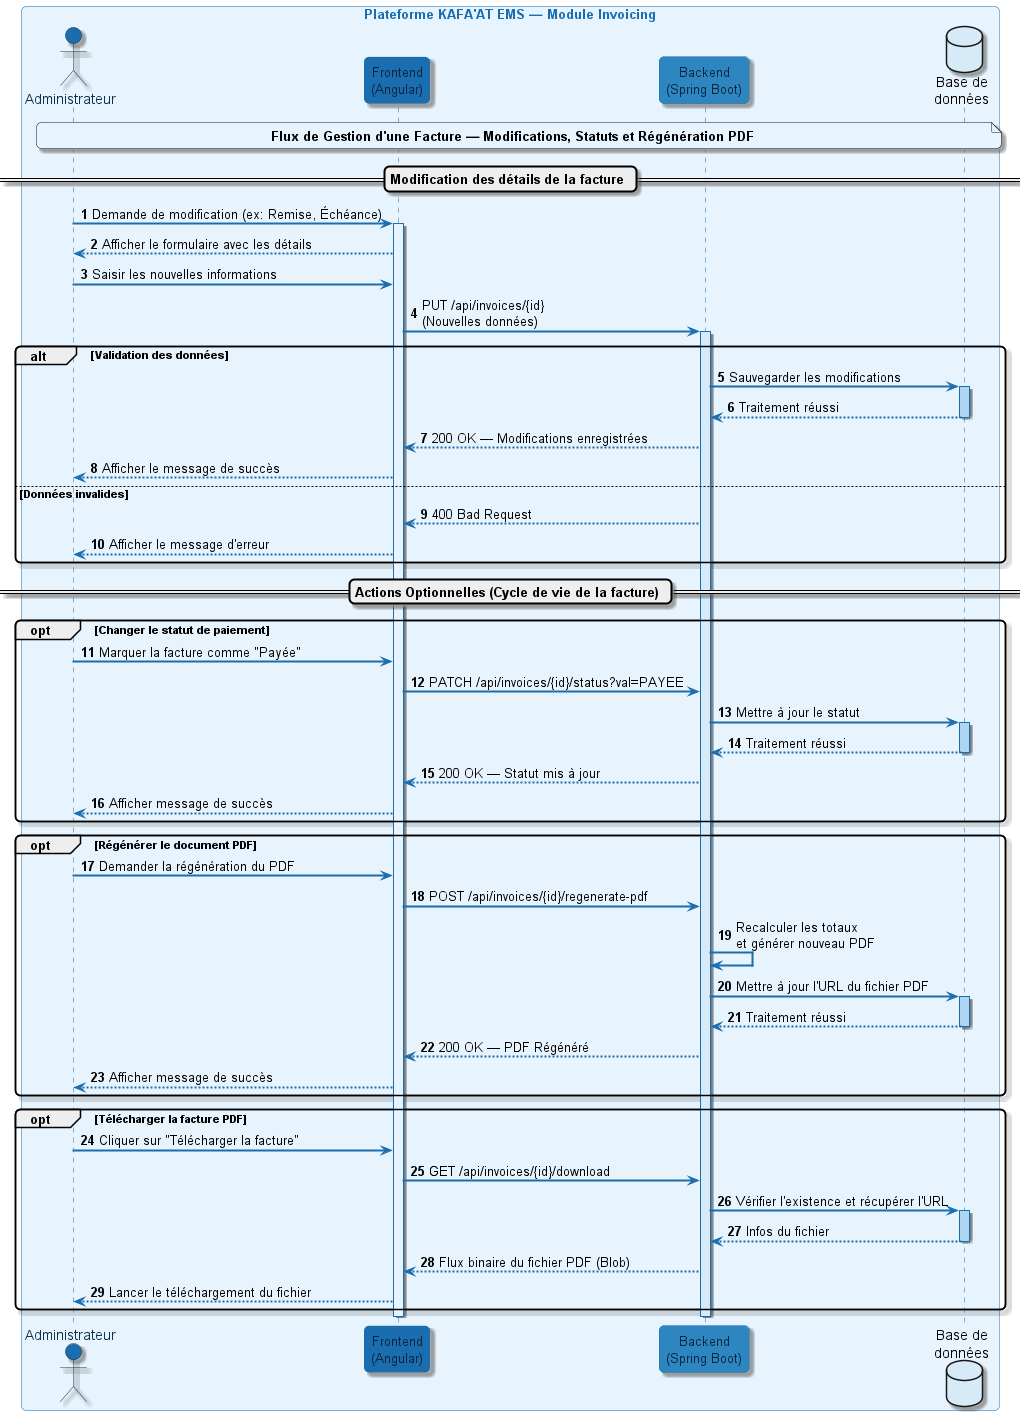
\includegraphics[width=1.0\textwidth]{images/sequence-gestion-facture.png}
    \vspace{-0.9cm}
    \caption{Diagramme de séquence de la gestion détaillée d'une facture}
    \label{fig:sequence_gestion_facture}
\end{figure}

\vspace{0.4cm}

\subsection{Diagrammes d'activité}

\vspace{-0.4cm}
Les diagrammes d'activité sont des diagrammes utilisés dans le langage de modélisation unifié (UML) pour représenter le flux d'activités ou de processus dans un système. Ils fournissent une vue visuelle de l'ordre des actions et des décisions prises au sein d'un système, en mettant l'accent sur les activités réalisées et les transitions entre ces activités. Les diagrammes d'activité sont constitués de nœuds d'activité, de transitions et de décisions. Les nœuds d'activité représentent les actions ou les étapes réalisées dans le système, tandis que les transitions indiquent le passage d'une activité à une autre. Les décisions permettent de représenter les points de branchement conditionnels dans le flux d'activité. 

Ces diagrammes sont particulièrement utiles pour modéliser des processus métier, des algorithmes ou des flux de contrôle dans un système. Ils permettent de visualiser le déroulement des activités et de comprendre les différentes étapes et décisions qui sont prises tout au long du processus. [11]

Dans le contexte de notre plateforme \textbf{KAFA'AT EMS}, ces diagrammes nous permettront de détailler avec précision la logique interne de nos processus clés, tels que la soumission et la validation des pointages, ainsi que le cycle complet de facturation.

\vspace{-0.4cm}
\subsubsection{Diagramme d'activité « Validation des pointages »}

\vspace{-0.4cm}
Ce premier diagramme d'activité modélise la logique métier et le flux de contrôle relatifs au suivi du temps de travail (Worktime). Afin d'illustrer clairement les responsabilités de chaque acteur, nous avons structuré ce diagramme en \textbf{couloirs d'activités (Swimlanes)} séparant l'Employé, le Système (Backend) et l'Administrateur.

L'algorithme se divise en deux phases critiques :
\begin{enumerate}[label=\textcolor{primaryBlue}{\arabic*.}, leftmargin=*]
    \item \textcolor{primaryBlue}{\textbf{Contrôle à la soumission :}} Le système agit comme un premier filtre. Il vérifie de manière autonome si le cumul des heures déclarées par l'employé ne dépasse pas le plafond journalier autorisé. Si la condition est respectée, le pointage est enregistré sous le statut \textit{SOUMIS}.
    \item \textcolor{primaryBlue}{\textbf{Arbre de décision administratif :}} Lors de la révision, l'administrateur dispose de trois branches conditionnelles : valider, refuser (avec motif) ou ajuster (Override). Chaque décision déclenche un comportement distinct dans le système, incluant la mise à jour des statuts et l'envoi de notifications asynchrones.
\end{enumerate}

\vspace{0.4cm}

\begin{figure}[H]
    \centering
    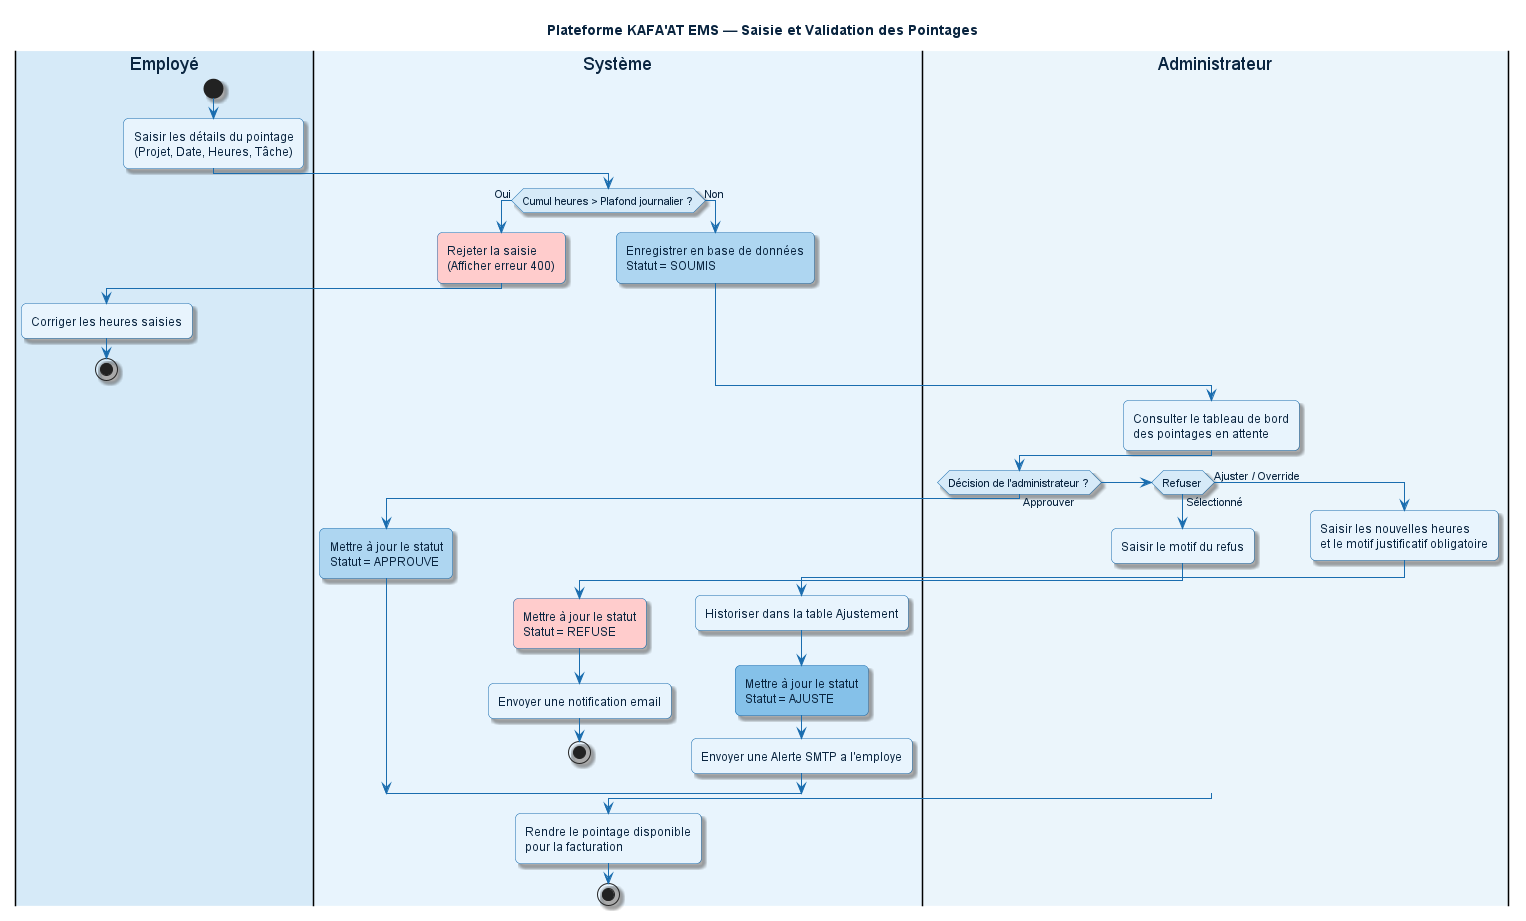
\includegraphics[width=1\textwidth]{images/activite-pointage.png}
    \vspace{-0.9cm}
    \caption{Diagramme d'activité avec Swimlanes : Validation des pointages}
    \label{fig:activite_pointage}
\end{figure}

\vspace{-0.6cm}

\subsubsection{Diagramme d'activité « Génération Massive des Factures »}

\vspace{-0.4cm}
Ce deuxième diagramme d'activité illustre le cœur algorithmique de notre module d'Invoicing. La génération massive des factures est une opération critique qui exige un traitement par lots (Batch processing) optimisé et une gestion rigoureuse des exceptions.

Le processus débute par une vérification stricte des habilitations de l'administrateur via son Token JWT. Le système extrait ensuite les pointages marqués comme \textit{APPROUVÉS}. L'algorithme principal repose sur une \textbf{structure itérative} qui traite chaque employé individuellement. Afin de prévenir les blocages de la chaîne d'exécution, le système intègre une gestion d'erreur interne : si un employé ne possède pas de paramètres financiers configurés (Groupe de Facturation/TJM manquant), une anomalie est journalisée et le système passe à l'itération suivante sans interruption.

Pour les profils valides, le moteur calcule les montants (HT et TTC), génère le document PDF via \textbf{JasperReports}, et prépare l'entité. Pour des raisons de performance, l'enregistrement en base de données s'effectue via une insertion en masse (\textit{Batch Insert}). 

Enfin, le flux d'exécution se scinde (\textit{Fork}) : l'envoi des courriels contenant les pièces jointes est délégué à un processus asynchrone, tandis que l'interface administrateur affiche instantanément un tableau de bord de synthèse détaillant le nombre de factures générées, le chiffre d'affaires total, et les éventuelles anomalies rencontrées.

\vspace{0.4cm}

\begin{figure}[H]
    \centering
    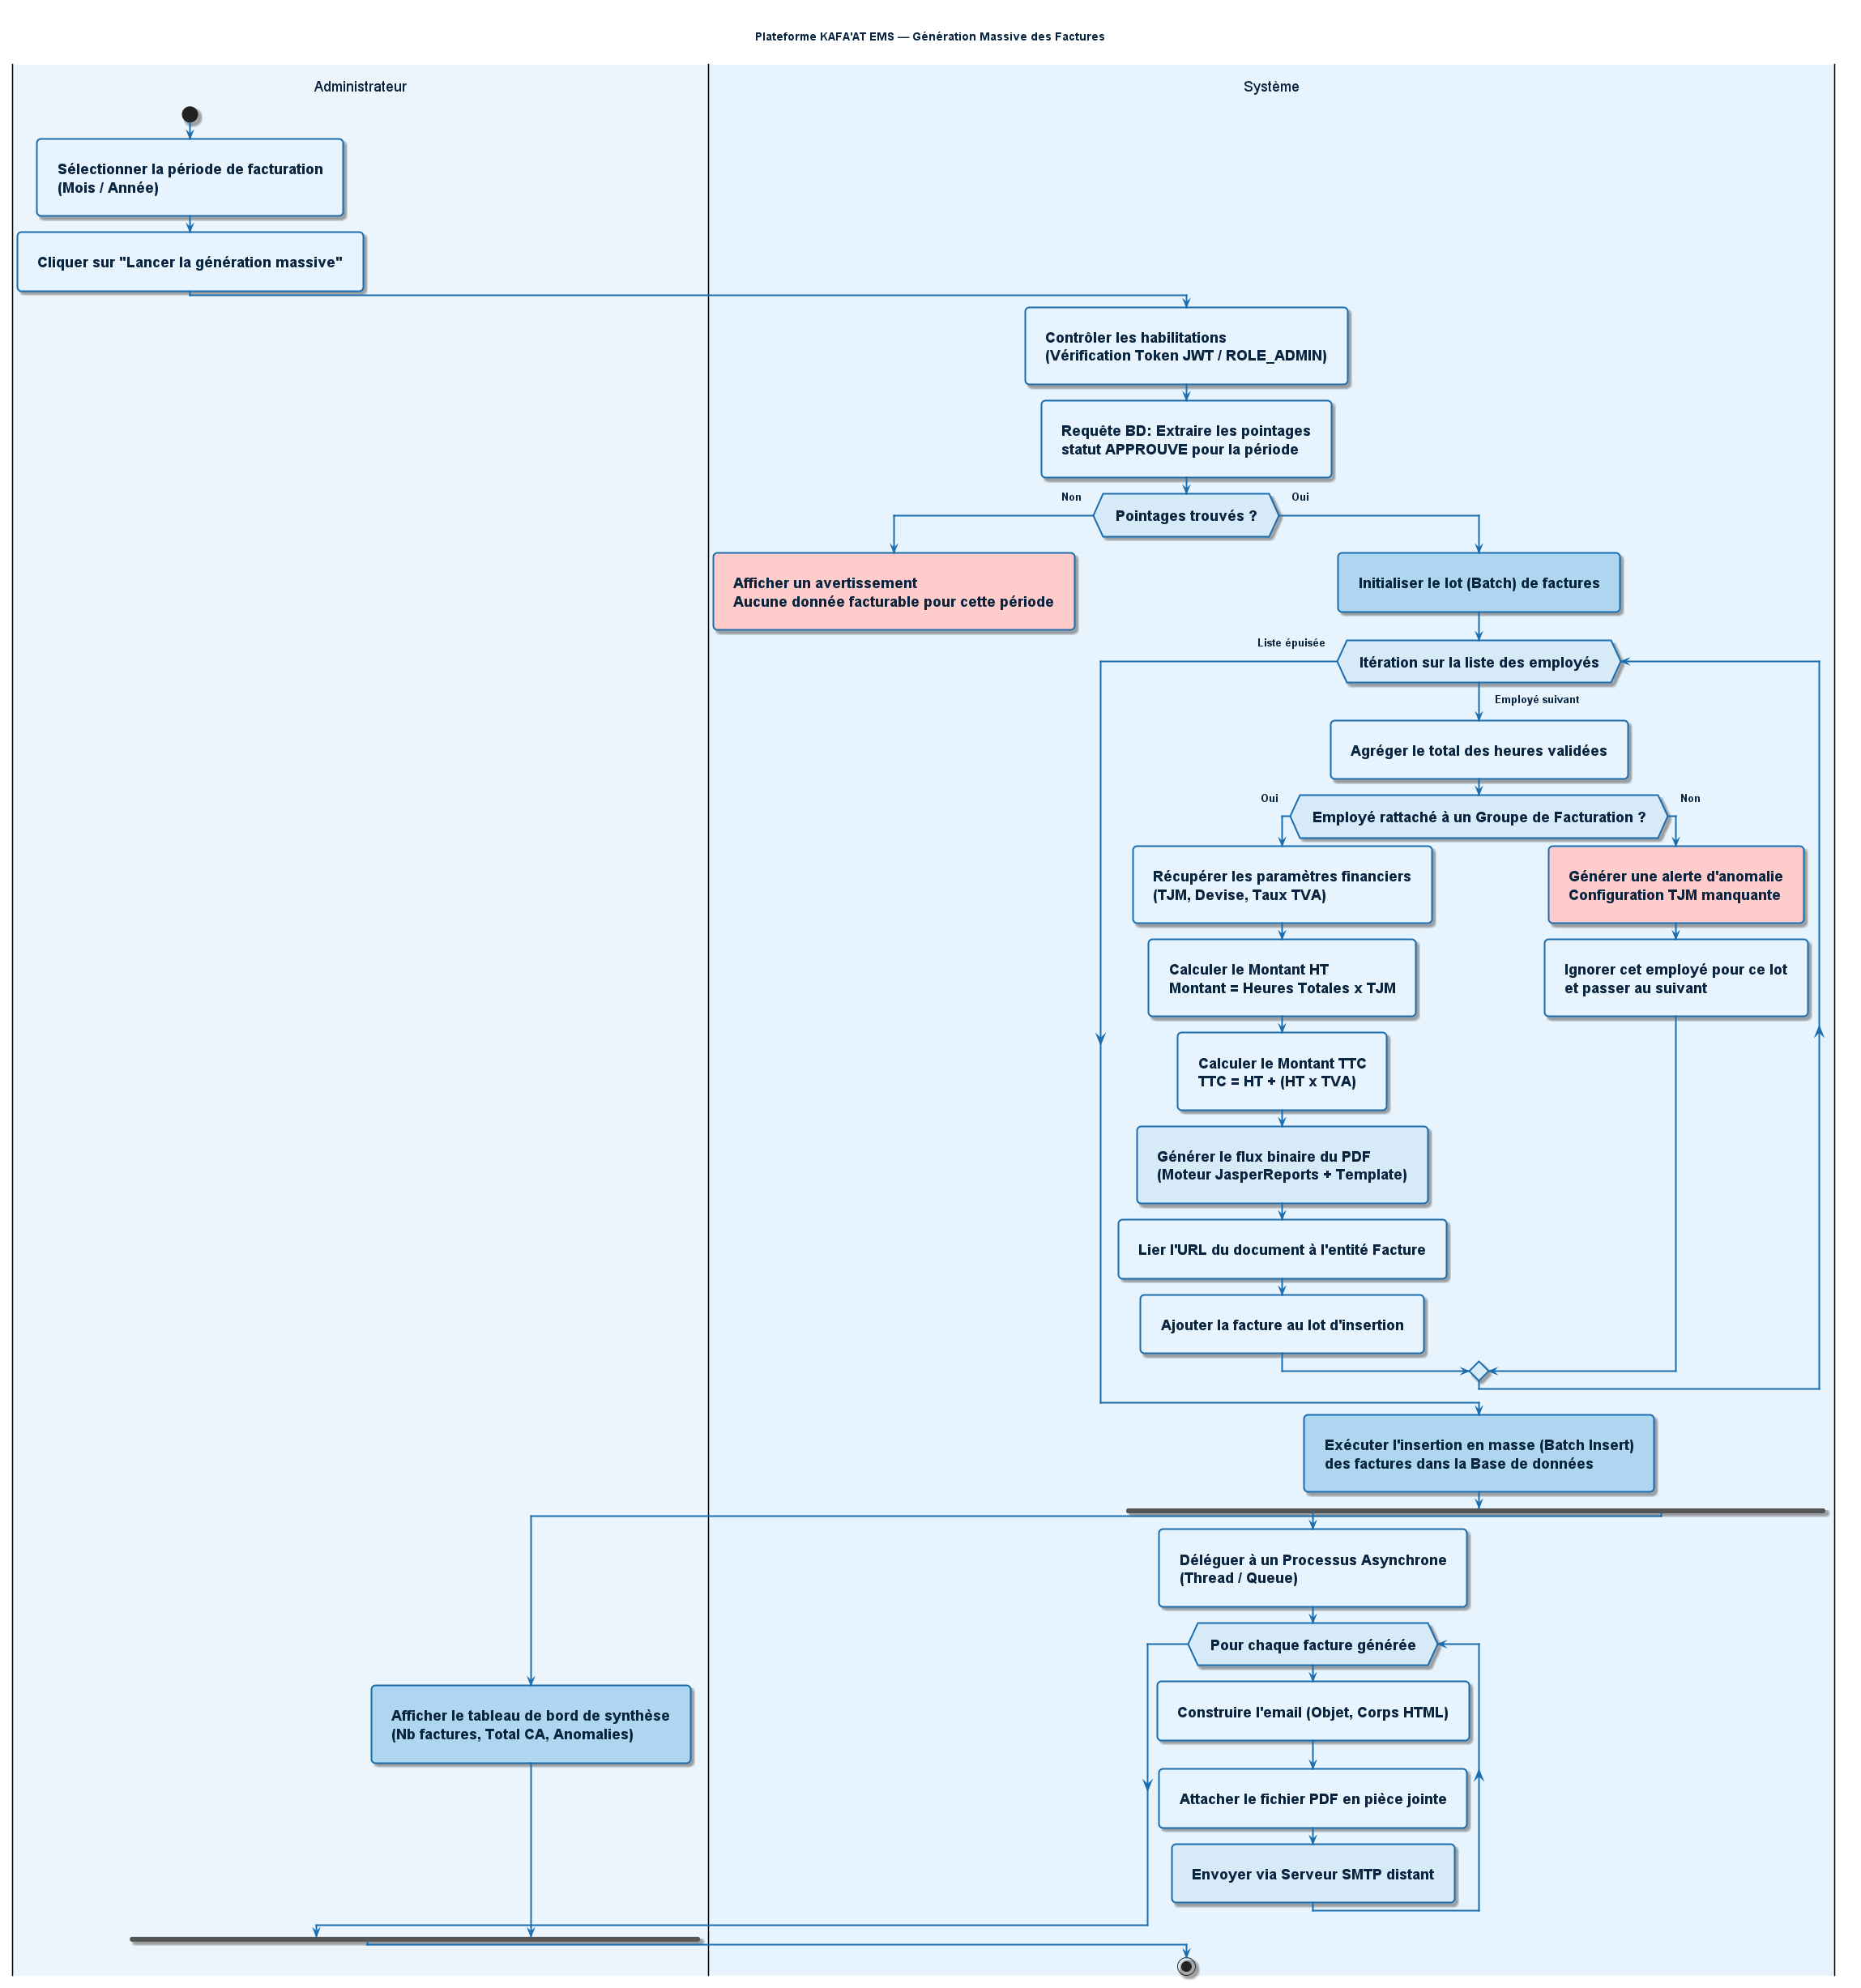
\includegraphics[width=1\textwidth]{images/activite-facturation.png}
    \vspace{-0.9cm}
    \caption{Diagramme d'activité détaillé : Moteur de génération massive des factures}
    \label{fig:activite_facturation}
\end{figure}

\vspace{-0.4cm}

\subsubsection{Diagramme d'activité « Suivi des factures »}

\vspace{-0.4cm}
Ce dernier diagramme d'activité modélise le cycle de vie post-génération d'une facture, englobant les opérations de suivi, d'encaissement et d'exportation. Il illustre les différentes branches décisionnelles qui s'offrent à l'administrateur lors de la consultation du module d'Invoicing.

Le processus débute par l'accès à la liste des factures. Si aucune facture spécifique n'est sélectionnée, l'administrateur a la possibilité de déclencher une extraction globale des données financières sous forme de fichier \textbf{Excel/CSV} pour un traitement externe.

Lorsqu'une facture est sélectionnée, le système oriente le flux selon l'action choisie :
\begin{itemize}[label=\textcolor{royalBlue}{\rule{1.2ex}{1.2ex}}, leftmargin=*, itemsep=0.1cm]
    \item \textcolor{primaryBlue}{\textbf{Recouvrement :}} Enregistrement des références de paiement, entraînant une mise à jour du statut vers \textit{PAYÉE} et la génération éventuelle d'un reçu.
    \item \textcolor{primaryBlue}{\textbf{Vérification des échéances :}} Le système effectue un contrôle logique. Si la facture est toujours en attente et que la date actuelle dépasse la date d'échéance convenue, le statut bascule automatiquement en \textit{EN\_RETARD} et une relance par courrier électronique est déclenchée.
    \item \textcolor{primaryBlue}{\textbf{Consultation :}} Téléchargement direct du document PDF archivé.
\end{itemize}

Indépendamment de l'action spécifique effectuée (modification ou consultation), le système clôture le processus en consignant l'opération dans un journal d'audit afin d'assurer une traçabilité complète des manipulations financières.

\vspace{0.4cm}

\begin{figure}[H]
    \centering
    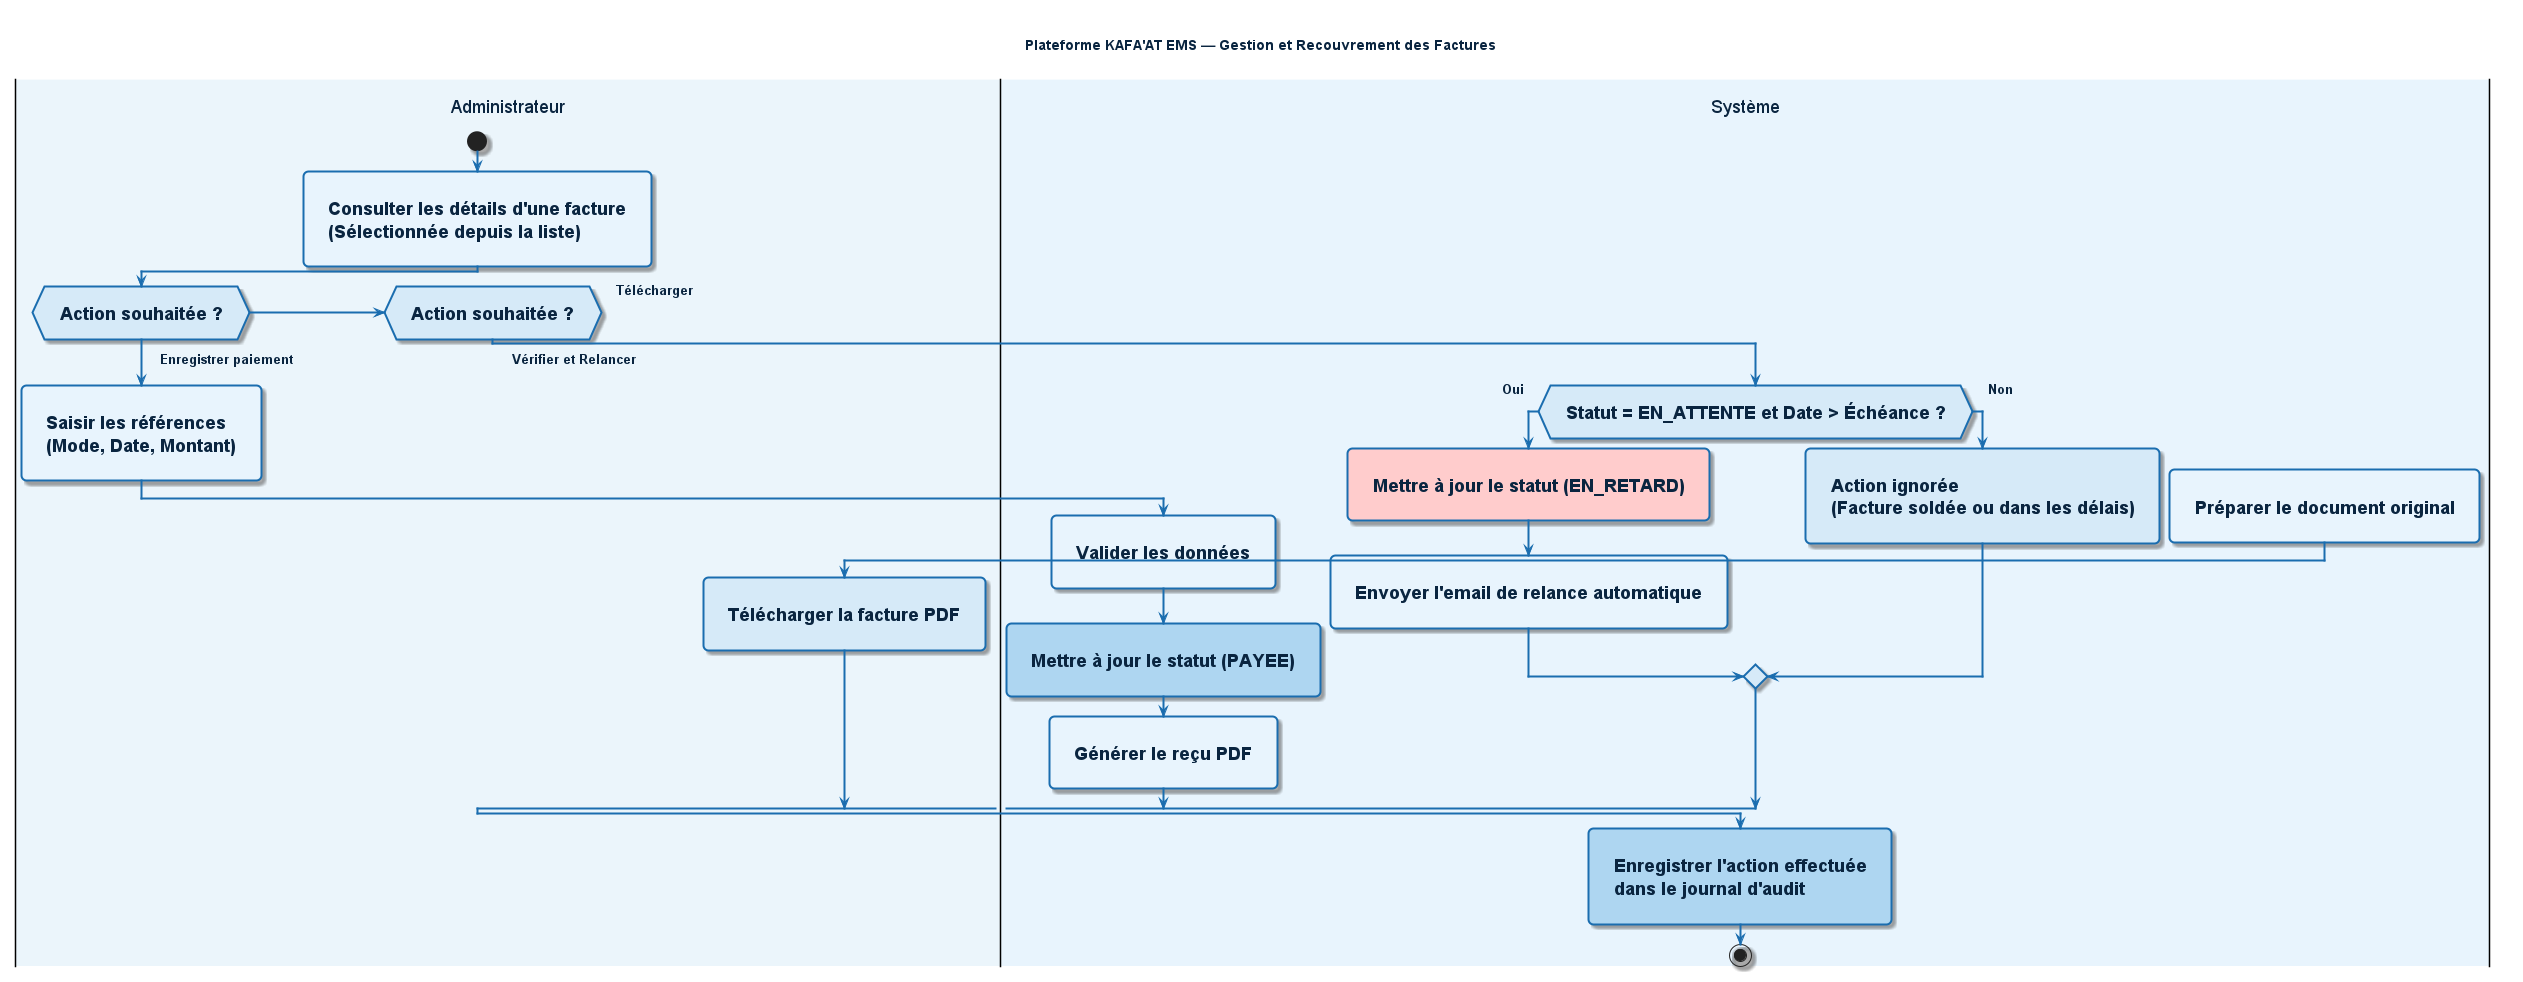
\includegraphics[width=1\textwidth]{images/activite-recouvrement.png} 
    \vspace{-0.9cm}
    \caption{Diagramme d'activité : Gestion, relances et recouvrement des factures}
    \label{fig:activite_recouvrement}
\end{figure}

\vspace{2.4cm}

\section*{Conclusion}
\addcontentsline{toc}{section}{Conclusion} % Bach t-ban f l'Fihres wakha ma3ndhach ra9m

\vspace{-0.4cm}
Dans ce chapitre, nous avons détaillé la phase de conception logicielle de notre projet en nous appuyant sur les standards du langage de modélisation UML. À travers l'élaboration progressive des diagrammes de cas d'utilisation, de classes, de séquence et d'activité, nous avons pu traduire les exigences métiers complexes des modules \textit{Invoicing} et \textit{Worktime} en spécifications techniques claires et rigoureuses.

Cette démarche de modélisation approfondie nous a permis de structurer une architecture robuste pour la plateforme KAFA'AT EMS. Nous avons ainsi pu anticiper la logique des processus critiques, tels que la validation hiérarchique des pointages, le moteur de génération massive des factures, et la gestion des habilitations, tout en garantissant la traçabilité et l'intégrité des données financières.

La conception conceptuelle et dynamique étant à présent achevée, ces modèles constitueront notre feuille de route pour la phase de développement. Le chapitre suivant sera ainsi consacré à la réalisation de l'application, où nous mettrons en œuvre cette architecture à travers l'implémentation des technologies choisies, notamment \textbf{Spring Boot} pour le Backend et \textbf{Angular} pour le Frontend.

% --- CHAPITRE 3 : START ---
\chapterpage{3}{Réalisation et Mise en œuvre}
\chapter{Réalisation et Mise en œuvre}

\vspace*{0.8cm} % <--- ZID HADI HNA BACH TB3ED "INTRODUCTION" 3LA L'KHAT ZRE9
\section*{Introduction}
\addcontentsline{toc}{section}{Introduction}

\vspace{-0.4cm}
Dans ce chapitre, nous abordons la concrétisation technique et la mise en œuvre de notre solution logicielle au sein de la plateforme KAFA'AT EMS. Nous commencerons par définir l'architecture globale du système, en justifiant les choix technologiques adoptés pour répondre aux exigences de performance, de sécurité et de scalabilité. Ensuite, nous détaillerons l'environnement de développement et les outils mis à profit lors de la réalisation. Enfin, nous présenterons les interfaces utilisateurs développées, en mettant l'accent sur l'ergonomie et l'expérience utilisateur (UX). Ce chapitre constitue ainsi la passerelle concrète entre la modélisation théorique et le produit final déployable.

\vspace{-0.4cm}
\section{Architecture de l'application}

\vspace{-0.4cm}
L'architecture logicielle structure le système en définissant ses composants, leurs responsabilités et leurs interactions. Pour les modules \textit{Invoicing} et \textit{Worktime} de la plateforme KAFA'AT EMS, nous avons adopté une approche multicouche, modulaire et hautement découplée. Cette configuration assure une stricte séparation des préoccupations (\textit{Separation of Concerns}) tout en optimisant la maintenance évolutive et la sécurité des flux.

La figure \ref{fig:architecture_globale} illustre cette architecture globale, mettant en évidence la communication fluide entre la couche de présentation (Angular), la logique métier centralisée (Spring Boot) et la persistance des données (PostgreSQL).

\vspace{0.1cm}
\begin{figure}[H]
    \centering
    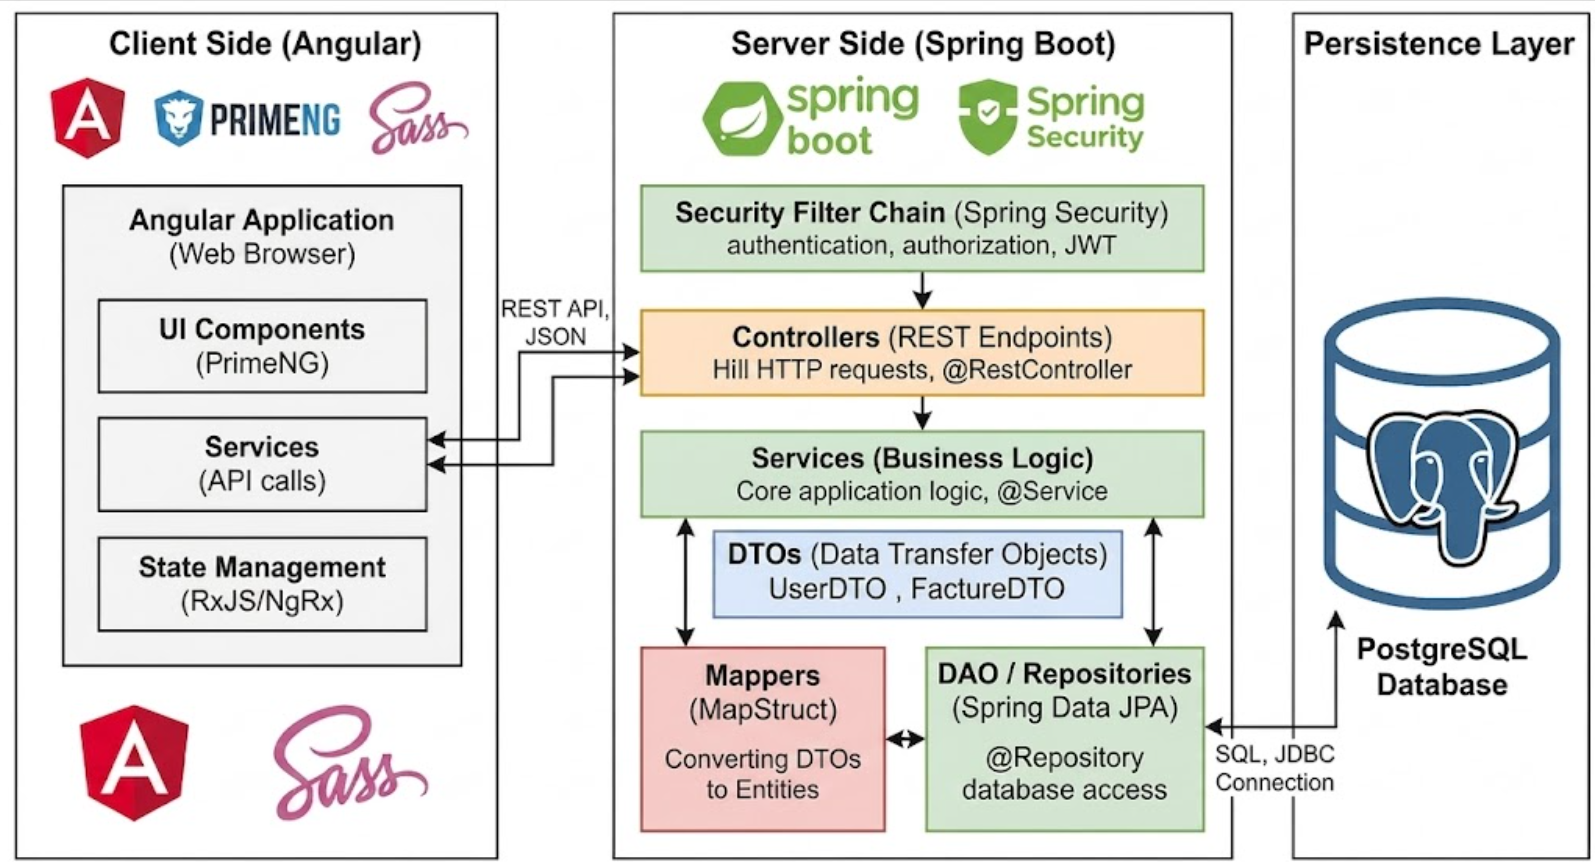
\includegraphics[width=1.0\textwidth]{images/architecture-globale-app.png}
    \vspace{-0.9cm}
    \caption{Architecture globale de l'application}
    \label{fig:architecture_globale}
\end{figure}
\vspace{0.2cm}

\subsection{Architecture Backend}

\vspace{-0.4cm}
Pour la partie serveur, nous avons opté pour le framework \textbf{Spring Boot} selon une architecture en couches (N-Tier). Cette approche isole la logique métier, sécurise les échanges et facilite la maintenance. Les couches s'articulent ainsi :

\begin{itemize}[label=\textcolor{royalBlue}{\rule{1.2ex}{1.2ex}}, leftmargin=*, itemsep=0.05cm]
    \item \textcolor{primaryBlue}{\textbf{Sécurité (Spring Security \& JWT) :}} Intercepte les requêtes pour assurer l'authentification et l'autorisation via les tokens JWT.
    \item \textcolor{primaryBlue}{\textbf{API REST (Controllers) :}} Expose les points d'entrée, valide les requêtes HTTP du client Angular et les achemine vers les services.
    \item \textcolor{primaryBlue}{\textbf{Couche Métier (Services) :}} Cœur de l'application, elle encapsule les algorithmes complexes (\textit{Invoicing}, \textit{Worktime}).
    \item \textcolor{primaryBlue}{\textbf{Objets de Transfert (DTOs \& MapStruct) :}} Limite les données exposées en convertissant automatiquement les Entités en DTOs.
    \item \textcolor{primaryBlue}{\textbf{Accès aux Données (Spring Data JPA) :}} Gère la persistance et les transactions avec la base de données \textbf{PostgreSQL}.
    \item \textcolor{primaryBlue}{\textbf{Génération (JasperReports) :}} Dédiée à la création dynamique des factures au format PDF.
\end{itemize}

Cette structuration rigoureuse garantit un code propre, testable et prêt à évoluer au sein de la plateforme KAFA'AT EMS.

\vspace{0.0cm}
\begin{figure}[H]
    \centering
    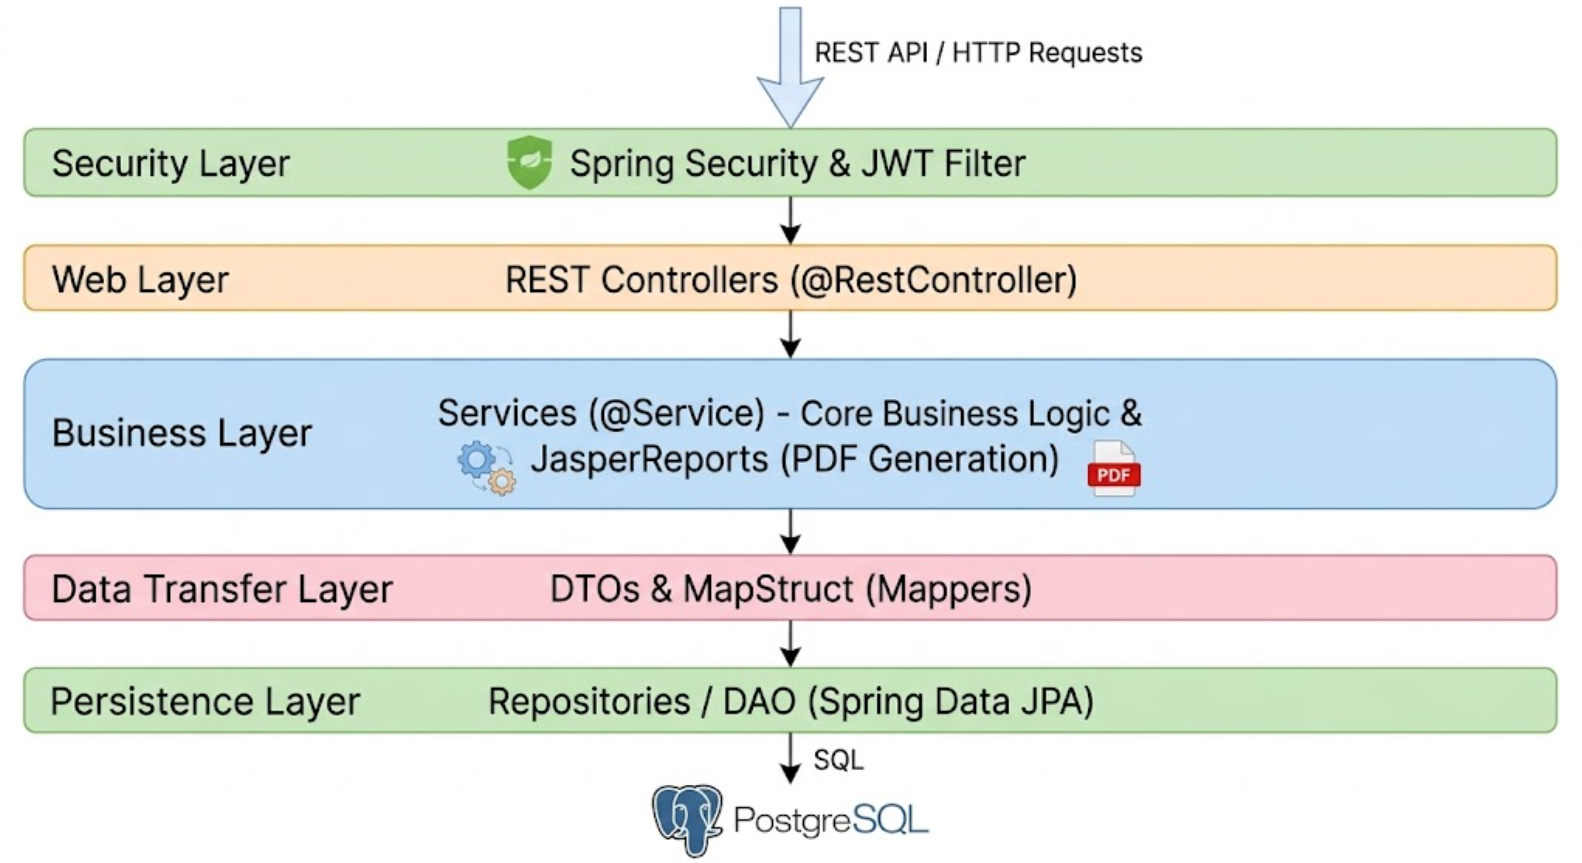
\includegraphics[width=0.99\textwidth]{images/architecture-backend.png}
    \vspace{-0.4cm}
    \caption{Architecture en couches du Backend (Spring Boot)}
    \label{fig:architecture_backend}
\end{figure}
\vspace{0.2cm}

\subsection{Architecture Frontend}

\vspace{-0.4cm}
Pour la partie cliente, notre application repose sur \textbf{Angular}, structuré selon une architecture orientée composants (Component-Based Architecture). Ce choix, couplé à \textbf{TypeScript} et à la bibliothèque graphique \textbf{PrimeNG}, garantit une interface (UI) réactive et modulaire pour les modules \textit{Invoicing} et \textit{Worktime}. L'architecture s'organise ainsi :

\begin{itemize}[label=\textcolor{royalBlue}{\rule{1.2ex}{1.2ex}}, leftmargin=*, itemsep=0.05cm]
    \item \textcolor{primaryBlue}{\textbf{Composants \& Templates (PrimeNG / SCSS) :}} Blocs de construction de l'interface. Chaque composant encapsule sa logique métier, sa structure HTML et son style, en intégrant les éléments riches de PrimeNG.
    \item \textcolor{primaryBlue}{\textbf{Services \& API Client :}} Classes encapsulant les appels HTTP vers le backend (Spring Boot), assurant la réutilisabilité et la stricte séparation des préoccupations.
    \item \textcolor{primaryBlue}{\textbf{Routage (SPA Routing) :}} Gère la navigation \textit{Single Page Application}, permettant des transitions fluides et sécurisées entre les différentes vues de la plateforme.
    \item \textcolor{primaryBlue}{\textbf{Programmation Réactive (RxJS) :}} Gestion asynchrone des flux de données (Observables) pour une mise à jour dynamique de l'interface en temps réel.
    \item \textcolor{primaryBlue}{\textbf{Modules \& Lazy Loading :}} Découpage fonctionnel du code permettant le chargement différé des ressources, optimisant ainsi les performances et le temps de réponse initial.
\end{itemize}

Cette architecture modulaire garantit une interface réactive et facilite la maintenance de la plateforme KAFA'AT EMS, comme illustré ci-dessous.

\vspace{0.2cm}
\begin{figure}[H]
    \centering
    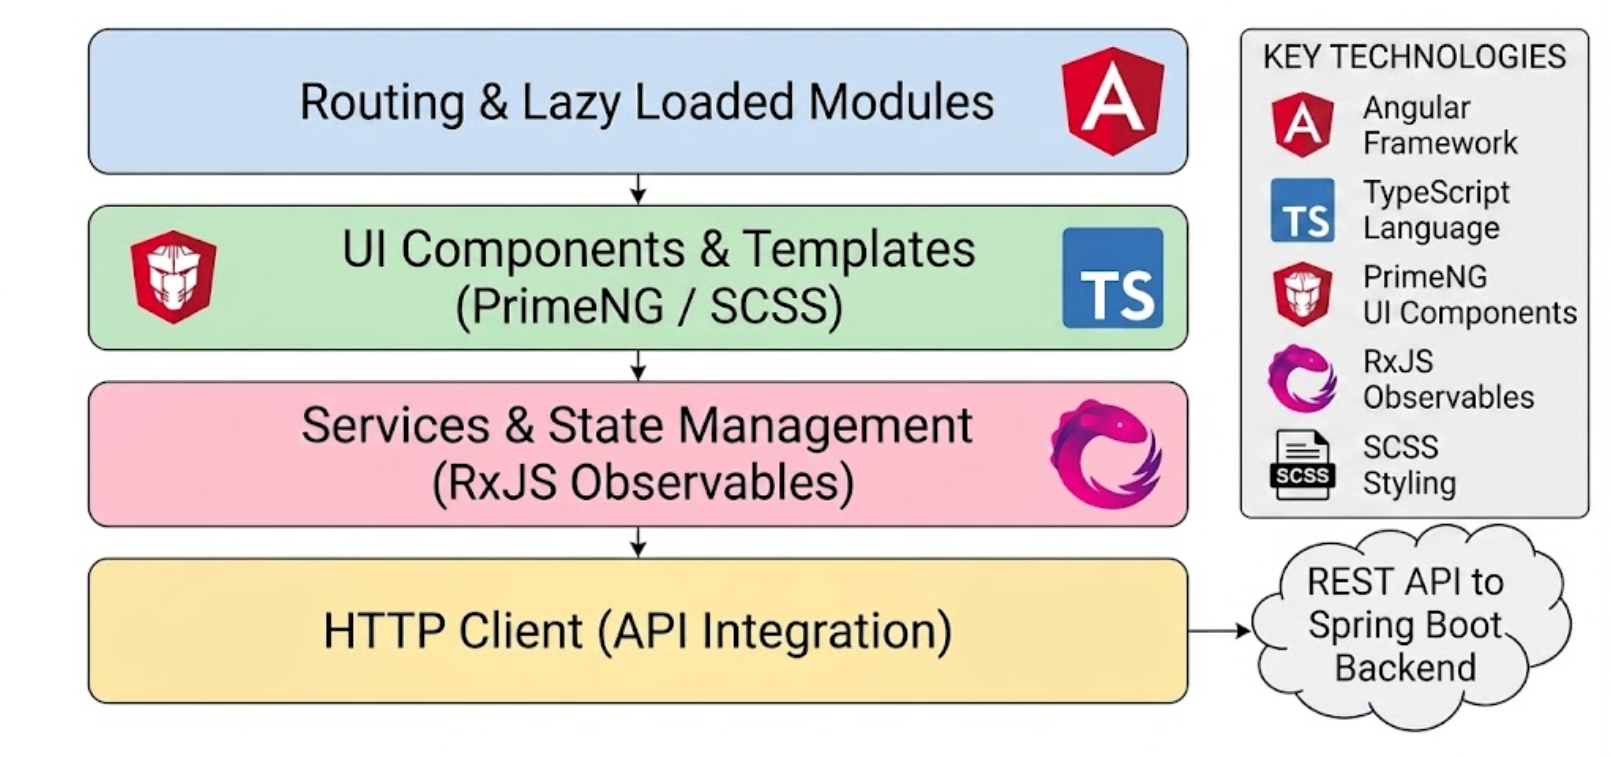
\includegraphics[width=1\textwidth]{images/architecture-frontend.png}
    \vspace{-0.9cm}
    \caption{Architecture interne de l'application cliente (Angular)}
    \label{fig:architecture_frontend}
\end{figure}
\vspace{0.2cm}

\section{Technologies et outils de développement}

\vspace{-0.4cm}
Cette section détaille l'écosystème technologique mis en place pour la réalisation de notre projet. Le choix de ces outils repose sur des critères stricts de performance, de sécurité et d'adéquation avec les standards de l'industrie logicielle.

\vspace{-0.4cm}
\subsection{Environnements logiciels}

\vspace{-0.4cm}
\subsubsection{IntelliJ IDEA}

\vspace{-0.4cm}

\begin{figure}[H]
    \centering
    
\includegraphics[width=0.20\textwidth]{images/intellij-logo.png}
    \vspace{-0.4cm}
    \caption{Logo d'IntelliJ IDEA}
    \label{fig:intellij}
\end{figure}

\vspace{-0.4cm}

IntelliJ IDEA a été sélectionné comme Environnement de Développement Intégré (IDE) principal pour la conception et l'implémentation de la couche backend (Spring Boot). 

Reconnu pour sa robustesse, cet outil a considérablement optimisé notre cycle de développement grâce à son analyse statique de code avancée, son autocomplétion intelligente et son intégration native avec l'écosystème Java. Il a particulièrement facilité le refactoring du code, la gestion des dépendances et le débogage complexe des algorithmes liés aux processus de facturation.

\vspace{-0.4cm}
\subsubsection{Visual Studio Code}

\vspace{-0.4cm}

\begin{figure}[H]
    \centering
    
\includegraphics[width=0.25\textwidth]{images/vscode-logo.png}
    \vspace{-0.4cm}
    \caption{Logo de Visual Studio Code}
    \label{fig:vscode}
\end{figure}

\vspace{-0.4cm}

Visual Studio Code (VS Code) a été adopté comme éditeur de choix pour l'implémentation de la partie frontend (Angular) de notre application. 

Sa légèreté, couplée à un écosystème d'extensions extrêmement riche, a permis d'adapter l'environnement aux exigences spécifiques de notre \textit{Stack} technologique. L'intégration native de terminaux multiples a grandement facilité l'exécution continue des commandes \textit{Angular CLI}. De plus, les extensions dédiées à TypeScript, le formatage automatique (Prettier) et l'intégration fluide de Git ont assuré un développement rapide, tout en maintenant une qualité de code optimale et une gestion efficace des \textit{Pull Requests}.

\vspace{-0.4cm}
\subsubsection{Swagger (OpenAPI)}

\vspace{-0.4cm}

\begin{figure}[H]
    \centering
    
\includegraphics[width=0.25\textwidth]{images/swagger-logo.png}
    \vspace{-0.4cm}
    \caption{Logo de Swagger}
    \label{fig:swagger}
\end{figure}

\vspace{-0.4cm}

Swagger a été intégré à notre backend Spring Boot afin de générer automatiquement une documentation interactive et standardisée de notre API REST, basée sur la spécification OpenAPI. 

Cet outil s'est avéré indispensable lors de la phase de développement pour l'exploration et le test direct des \textit{Endpoints} (notamment ceux liés aux processus d'Invoicing et de Worktime) sans nécessiter de client externe. En fournissant un contrat d'interface clair, Swagger a considérablement fluidifié l'intégration logicielle et la communication technique entre notre logique serveur et les services clients de l'application Angular.

\vspace{-0.4cm}
\subsubsection{Apache Tomcat}

\vspace{-0.4cm}

\begin{figure}[H]
    \centering
    
\includegraphics[width=0.20\textwidth]{images/tomcat-logo.png}
    \vspace{-0.4cm}
    \caption{Logo d'Apache Tomcat}
    \label{fig:tomcat}
\end{figure}

\vspace{-0.4cm}

Apache Tomcat est un conteneur de servlets et un serveur web open-source de référence pour l'environnement Java. Dans le cadre de notre projet, Tomcat a été utilisé dans sa version embarquée (\textit{embedded}) nativement fournie par le framework Spring Boot.

Cette intégration transparente nous a affranchis des configurations fastidieuses liées au déploiement d'un serveur externe. Elle a permis de lancer, de tester et de déployer nos API REST (gérant la logique complexe des modules \textit{Invoicing} et \textit{Worktime}) de manière totalement autonome, légère et performante tout au long de notre cycle de développement.

\vspace{-0.4cm}
\subsubsection{Docker}

\vspace{-0.4cm}

\begin{figure}[H]
    \centering
    
\includegraphics[width=0.17\textwidth]{images/docker-logo.png}
    \vspace{-0.4cm}
    \caption{Logo de Docker}
    \label{fig:docker}
\end{figure}

\vspace{-0.4cm}

Afin de garantir un environnement de développement et de déploiement standardisé, nous avons intégré Docker, une plateforme de conteneurisation incontournable. Son utilisation s'est articulée autour de trois axes majeurs au sein de notre projet :

\begin{itemize}[label=\textcolor{royalBlue}{\rule{1.2ex}{1.2ex}}, leftmargin=*, itemsep=0.05cm]
    \item \textcolor{primaryBlue}{\textbf{Base de données locale (\textit{Docker Compose}) :}} Instanciation rapide de notre base de données PostgreSQL via un fichier \texttt{docker-compose.yml}, éliminant ainsi le besoin d'installations lourdes sur la machine locale.
    \item \textcolor{primaryBlue}{\textbf{Conteneurisation de l'application (\textit{Dockerfile}) :}} Création d'images sur mesure pour le backend (Spring Boot) et le frontend (Angular), garantissant une isolation parfaite et une portabilité totale des livrables.
    \item \textcolor{primaryBlue}{\textbf{Intégration Continue (CI/CD) :}} Alignement avec les pratiques \textit{DevOps} de l'équipe NTT DATA, en facilitant la création et le déploiement automatisé de la plateforme KAFA'AT EMS sur les environnements de test et de production.
\end{itemize}

Cette approche moderne a considérablement optimisé notre flux de travail, résolvant les problèmes classiques de compatibilité inter-environnements et apportant une robustesse de niveau entreprise à l'ensemble du système.

\vspace{-0.4cm}
\subsubsection{Apache Maven}

\vspace{-0.4cm}

\begin{figure}[H]
    \centering
    
\includegraphics[width=0.20\textwidth]{images/maven-logo.png}
    \vspace{-0.4cm}
    \caption{Logo d'Apache Maven}
    \label{fig:maven}
\end{figure}

\vspace{-0.4cm}

Apache Maven a été utilisé comme outil principal d'automatisation de compilation et de gestion des dépendances pour notre backend Spring Boot. 

Via son fichier de configuration central \texttt{pom.xml}, Maven a structuré le projet et géré de manière transparente l'intégration des bibliothèques tierces indispensables à notre logique métier (telles que \textit{Spring Security} pour l'authentification JWT, \textit{MapStruct} pour le mappage des DTOs, et \textit{JasperReports} pour la facturation). Il a automatisé notre processus de \textit{build}, garantissant ainsi une construction fiable, reproductible et prête pour l'intégration continue.

\vspace{-0.4cm}
\subsubsection{Node.js}

\vspace{-0.4cm}

\begin{figure}[H]
    \centering
    
\includegraphics[width=0.20\textwidth]{images/nodejs-logo.png}
    \vspace{-0.4cm}
    \caption{Logo de Node.js}
    \label{fig:nodejs}
\end{figure}

\vspace{-0.4cm}

Bien que notre logique serveur soit gérée par Spring Boot, l'environnement Node.js s'est avéré indispensable pour la partie cliente de notre application. Dans notre architecture, Node.js n'agit pas comme un serveur web de production, mais exclusivement comme moteur d'exécution en arrière-plan pour l'écosystème de développement frontend. Il fournit l'environnement nécessaire au fonctionnement d'Angular CLI, permettant la compilation à la volée du code TypeScript, la minification des ressources et le lancement du serveur de développement local.

\vspace{-0.4cm}
\subsubsection{NPM (Node Package Manager)}

\vspace{-0.4cm}

\begin{figure}[H]
    \centering
    
\includegraphics[width=0.17\textwidth]{images/npm-logo.png}
    \vspace{-0.4cm}
    \caption{Logo de NPM}
    \label{fig:npm}
\end{figure}

\vspace{-0.4cm}

NPM intervient comme le gestionnaire de paquets standard pour notre couche frontend, jouant un rôle symétrique à celui de Maven pour le backend. Il a facilité la résolution, l'installation et la gestion des versions de l'ensemble des dépendances Angular requises par notre interface. Via le fichier de configuration \texttt{package.json}, NPM nous a permis d'intégrer efficacement des bibliothèques clés pour l'ergonomie de l'application, telles que le framework UI \textit{PrimeNG} pour la création des composants visuels, et \textit{RxJS} pour la gestion réactive des événements.

\vspace{-0.4cm}
\subsubsection{JWT (JSON Web Token)}

\vspace{-0.4cm}
\begin{figure}[H]
    \centering
    
\includegraphics[width=0.20\textwidth]{images/jwt-logo.png}
    \vspace{-0.4cm}
    \caption{Logo de JWT}
    \label{fig:jwt}
\end{figure}

\vspace{-0.4cm}

Dans le cadre de la sécurisation de notre architecture distribuée, JWT a été adopté comme standard pour gérer l'authentification et l'autorisation entre notre client Angular et l'API REST Spring Boot. Contrairement aux sessions classiques, JWT nous a permis de mettre en place une approche \textit{stateless} (sans état). Une fois l'utilisateur authentifié, le jeton généré encapsule ses informations et ses rôles sous forme chiffrée. Il est ensuite transmis via les en-têtes HTTP (\textit{Headers}), garantissant ainsi un accès hautement sécurisé aux ressources sensibles des modules \textit{Invoicing} et \textit{Worktime} sans surcharger la mémoire du serveur.

\vspace{-0.4cm}
\subsubsection{Postman}

\vspace{-0.4cm}

\begin{figure}[H]
    \centering
    
\includegraphics[width=0.20\textwidth]{images/postman-logo.png}
    \vspace{-0.4cm}
    \caption{Logo de Postman}
    \label{fig:postman}
\end{figure}

\vspace{-0.4cm}

Postman s'est imposé comme l'outil de prédilection pour le test, le débogage et la validation de nos API REST. Indépendamment du développement de l'interface graphique (Angular), Postman nous a permis d'interroger directement les \textit{endpoints} exposés par notre backend Spring Boot. 

Grâce à cet outil, nous avons pu simuler des requêtes HTTP complexes, valider la conformité des structures de données JSON (DTOs) entrantes et sortantes liées aux modules \textit{Invoicing} et \textit{Worktime}. De plus, Postman a été crucial pour tester notre couche de sécurité, en nous permettant d'injecter manuellement les jetons JWT dans les en-têtes d'autorisation (\textit{Authorization Headers}) afin de vérifier les restrictions d'accès selon les rôles utilisateurs.

\subsubsection{PlantUML}

\vspace{-0.4cm}

\begin{figure}[H]
    \centering
    
\includegraphics[width=0.20\textwidth]{images/plantuml-logo.png}
    \vspace{-0.4cm}
    \caption{Logo de PlantUML}
    \label{fig:plantuml}
\end{figure}

\vspace{-0.4cm}

Pour la phase d'analyse et de conception (détaillée dans le chapitre précédent), nous avons délibérément écarté les logiciels de modélisation graphique classiques au profit de PlantUML. Cet outil open-source permet de générer des diagrammes UML (cas d'utilisation, séquences, activités) à partir d'un langage de description textuel clair. Cette approche novatrice de \textit{« Diagram as Code »} a offert des avantages considérables : elle a permis un versionnage fluide de nos modèles via Git, facilité les revues lors des \textit{Pull Requests}, et garanti une esthétique uniforme et professionnelle pour l'ensemble des schémas architecturaux du projet.

\vspace{-0.3cm}

\subsection{Frameworks et technologies clés}

\vspace{-0.4cm}
\subsubsection{Spring Boot}

\vspace{-0.4cm}

\begin{figure}[H]
    \centering
    
\includegraphics[width=0.20\textwidth]{images/springboot-logo.png}
    \vspace{-0.4cm}
    \caption{Logo de Spring Boot}
    \label{fig:springboot}
\end{figure}

\vspace{-0.4cm}

Spring Boot constitue l'épine dorsale de notre architecture backend. Ce framework a été privilégié pour sa capacité à amorcer rapidement des applications Java robustes grâce à son mécanisme d'auto-configuration et son conteneur d'inversion de contrôle (IoC). Au sein de la plateforme KAFA'AT EMS, il nous a permis de nous affranchir des configurations fastidieuses pour nous concentrer exclusivement sur la logique métier complexe des modules \textit{Invoicing} et \textit{Worktime}. Il a grandement facilité l'implémentation et l'exposition de nos services via des API RESTful performantes, autonomes et prêtes pour la production.

\vspace{-0.4cm}
\subsubsection{Spring Security}

\vspace{-0.4cm}

\begin{figure}[H]
    \centering
    
\includegraphics[width=0.20\textwidth]{images/springsecurity-logo.png}
    \vspace{-0.4cm}
    \caption{Logo de Spring Security}
    \label{fig:springsecurity}
\end{figure}

\vspace{-0.4cm}

Spring Security est le module incontournable que nous avons intégré pour assurer la protection globale de notre backend. Contrairement aux approches monolithiques traditionnelles basées sur les sessions, nous l'avons configuré pour opérer de manière \textit{stateless} (sans état) en parfaite synergie avec notre système de jetons JWT. Ce framework nous a permis d'implémenter un contrôle d'accès granulaire basé sur les rôles (RBAC). Ainsi, il garantit que chaque requête HTTP ciblant des ressources sensibles (comme les données de facturation ou les pointages) soit rigoureusement interceptée, authentifiée et autorisée avant d'atteindre nos contrôleurs REST.

\vspace{-0.4cm}
\subsubsection{Spring Data JPA}

\vspace{-0.4cm}

\begin{figure}[H]
    \centering
    
\includegraphics[width=0.15\textwidth]{images/springdatajpa-logo.png}
    \vspace{-0.4cm}
    \caption{Logo de Spring Data JPA}
    \label{fig:springdatajpa}
\end{figure}

\vspace{-0.4cm}

Pour la couche de persistance, nous avons exploité Spring Data JPA, soutenu en arrière-plan par l'ORM Hibernate. Ce composant stratégique nous a permis d'abstraire la complexité des requêtes SQL et d'interagir avec notre base de données PostgreSQL via une approche orientée objet. En étendant simplement les interfaces \texttt{JpaRepository}, nous avons drastiquement réduit le code \textit{boilerplate} pour les opérations CRUD. De plus, Spring Data JPA a assuré une gestion transactionnelle rigoureuse, un aspect critique pour maintenir l'intégrité des données financières dans le module \textit{Invoicing} et l'exactitude des pointages dans le module \textit{Worktime}.

\vspace{-0.4cm}
\subsubsection{Angular}

\vspace{-0.4cm}

\begin{figure}[H]
    \centering
    
\includegraphics[width=0.10\textwidth]{images/angular-logo.png}
    \vspace{-0.4cm}
    \caption{Logo d'Angular}
    \label{fig:angular}
\end{figure}

\vspace{-0.4cm}

Côté client, Angular s'est imposé comme le framework de choix pour concevoir l'interface utilisateur de notre plateforme. En s'appuyant sur la robustesse du typage strict de TypeScript, il nous a permis de structurer une \textit{Single Page Application} (SPA) modulaire. Grâce à sa gestion efficace de l'état asynchrone et à l'intégration de bibliothèques tierces comme \textit{PrimeNG}, Angular a offert une expérience utilisateur fluide et hautement réactive. Il a servi de pont direct avec notre backend, consommant efficacement les API REST sécurisées par JWT pour afficher et manipuler dynamiquement les tableaux de bord et les interfaces de gestion.

\vspace{-0.4cm}
\subsubsection{Sass (SCSS)}

\vspace{-0.4cm}

\begin{figure}[H]
    \centering
    
\includegraphics[width=0.10\textwidth]{images/sass-logo.png}
    \vspace{-0.4cm}
    \caption{Logo de Sass}
    \label{fig:sass}
\end{figure}

\vspace{-0.4cm}

Sass (Syntactically Awesome Style Sheets) a été adopté comme préprocesseur CSS pour la partie cliente de notre application. Intégré nativement dans notre projet Angular via l'extension \texttt{.scss}, il nous a permis de pallier les limitations du CSS classique. L'utilisation de variables, de \textit{mixins} et de l'imbrication (\textit{nesting}) a grandement facilité la personnalisation des composants graphiques de \textit{PrimeNG}. Cet outil a garanti le respect de la charte graphique de la plateforme KAFA'AT EMS, tout en produisant un code de style modulaire, réutilisable et hautement maintenable.

\vspace{-0.3cm}
\subsection{Frameworks de tests et Assurance Qualité}

\vspace{-0.4cm}
\subsubsection{JUnit}

\vspace{-0.4cm}

\begin{figure}[H]
    \centering
    
\includegraphics[width=0.20\textwidth]{images/junit-logo.png}
    \vspace{-0.4cm}
    \caption{Logo de JUnit}
    \label{fig:junit}
\end{figure}

\vspace{-0.4cm}

JUnit a été utilisé comme framework de référence pour l'écriture et l'exécution des tests unitaires de notre backend Spring Boot. Il nous a permis de valider rigoureusement la logique métier et les algorithmes de calcul complexes des modules \textit{Invoicing} et \textit{Worktime}. Grâce à son riche écosystème d'annotations et d'assertions, nous avons pu garantir la fiabilité du code serveur et prévenir les régressions lors des phases de refactoring.

\vspace{-0.4cm}
\subsubsection{Mockito}

\vspace{-0.4cm}

\begin{figure}[H]
    \centering
    
\includegraphics[width=0.20\textwidth]{images/mockito-logo.png}
    \vspace{-0.4cm}
    \caption{Logo de Mockito}
    \label{fig:mockito}
\end{figure}

\vspace{-0.4cm}

En complément de JUnit, Mockito s'est avéré indispensable pour isoler le code en cours de test. Ce framework de \textit{mocking} nous a permis de simuler le comportement des dépendances externes (telles que les \textit{Repositories} de la base de données ou les appels d'API tierces). En créant des objets factices (\textit{mocks}), nous avons pu exécuter des tests unitaires rapides, déterministes et totalement indépendants de l'état de notre base de données PostgreSQL.

\vspace{-0.4cm}
\subsubsection{Jest}

\vspace{-0.4cm}

\begin{figure}[H]
    \centering
    
\includegraphics[width=0.20\textwidth]{images/jest-logo.png}
    \vspace{-0.4cm}
    \caption{Logo de Jest}
    \label{fig:jest}
\end{figure}

\vspace{-0.4cm}

Pour garantir la qualité de la partie cliente (Angular), nous avons intégré Jest comme environnement de test. Préféré pour sa rapidité d'exécution et sa configuration minimale, Jest a facilité les tests de nos composants graphiques (\textit{UI}) et de nos services TypeScript. Ses capacités de simulation avancées et ses rapports de couverture de code ont grandement contribué à maintenir la stabilité et la réactivité de l'interface de la plateforme KAFA'AT EMS.

\vspace{-0.3cm}
\subsection{Outils de gestion de projet et de collaboration}

\vspace{-0.4cm}
\subsubsection{Jira Software}

\vspace{-0.4cm}

\begin{figure}[H]
    \centering
    
\includegraphics[width=0.30\textwidth]{images/jira-logo.png}
    \vspace{-0.4cm}
    \caption{Logo de Jira Software}
    \label{fig:jira}
\end{figure}

\vspace{-0.4cm} 

Dans le cadre de l'adoption de la méthodologie Agile (Scrum) au sein de l'environnement NTT DATA, Jira Software s'est imposé comme l'outil central de notre gestion de projet. 

Il nous a permis de structurer le développement des modules \textit{Invoicing} et \textit{Worktime} sous forme de \textit{Sprints} itératifs. Grâce à ses tableaux de bord (Kanban/Scrum), nous avons pu gérer efficacement le \textit{Backlog} du produit, suivre l'avancement des \textit{User Stories} et coordonner les tâches quotidiennes. Jira a ainsi garanti une visibilité totale sur le cycle de vie des fonctionnalités et a assuré une collaboration transparente et continue avec l'équipe d'encadrement.

\vspace{-0.4cm}
\subsection{Contrôle de version et collaboration}

\vspace{-0.4cm}
\subsubsection{Git}

\vspace{-0.4cm}

\begin{figure}[H] 
    \centering
    
\includegraphics[width=0.15\textwidth]{images/git-logo.png}
    \vspace{-0.4cm}
    \caption{Logo de Git}
    \label{fig:git}
\end{figure}

\vspace{-0.4cm}

Git a été adopté comme système de contrôle de version décentralisé pour l'ensemble de notre code source. Cet outil standard nous a permis de suivre minutieusement l'évolution des composants frontend et backend. Grâce à une gestion stricte des branches (\textit{Branching}), nous avons pu développer les nouvelles fonctionnalités (comme la génération des factures ou la gestion des pointages) de manière totalement isolée, évitant ainsi les conflits lors de l'intégration continue.

\vspace{-0.4cm}
\subsubsection{GitLab}

\vspace{-0.4cm}

\begin{figure}[H]
    \centering
    
\includegraphics[width=0.20\textwidth]{images/gitlab-logo.png}
    \vspace{-0.4cm}
    \caption{Logo de GitLab}
    \label{fig:gitlab}
\end{figure}

\vspace{-0.4cm}

En parfaite synergie avec Git, GitLab a été utilisé comme plateforme centralisée pour l'hébergement de nos dépôts sécurisés. Au-delà du simple stockage, GitLab a structuré notre flux de travail collaboratif au sein de l'environnement NTT DATA. L'utilisation des \textit{Merge Requests} a grandement facilité les revues de code avec l'encadrement professionnel. De plus, ses fonctionnalités natives de CI/CD se sont avérées indispensables pour l'automatisation de nos pipelines de tests et le déploiement des modules de la plateforme KAFA'AT EMS.

\vspace{-0.3cm}
\section{Présentation des interfaces de l'application}

\vspace{-0.4cm}
Cette section est consacrée à la présentation des interfaces graphiques (UI) développées pour notre application. Conçues à l'aide du framework Angular et enrichies par la bibliothèque de composants PrimeNG, ces interfaces ont été pensées pour offrir une expérience utilisateur (UX) optimale, ergonomique et parfaitement alignée avec la charte graphique de l'environnement NTT DATA. 

Les captures d'écran suivantes illustrent l'aboutissement de notre travail de conception, en mettant en évidence les fonctionnalités clés et les interactions offertes aux différents acteurs utilisant les modules \textit{Invoicing} et \textit{Worktime} au sein de la plateforme KAFA'AT EMS.



\end{document}